%&preformat-disser
\RequirePackage[l2tabu,orthodox]{nag} % Раскомментировав, можно в логе получать рекомендации относительно правильного использования пакетов и предупреждения об устаревших и нерекомендуемых пакетах
% Формат А4, 14pt (ГОСТ Р 7.0.11-2011, 5.3.6)
\documentclass[a4paper,14pt,oneside,openany]{memoir}

% все настройки 
% файл с настройками документов, для того чтобы транслировать разные настройки по нескольким документам
% rnt 2018

% version definition
\newcommand{\unf}{Unifloc 7.9 VBA}

%% Режим черновика
\makeatletter
\@ifundefined{c@draft}{
  \newcounter{draft}
  \setcounter{draft}{0}  % 0 --- чистовик (максимальное соблюдение ГОСТ)
                         % 1 --- черновик (отклонения от ГОСТ, но быстрая сборка итоговых PDF)
}{}
\makeatother


%%% Использование в xelatex и lualatex семейств шрифтов %%%
\makeatletter
\@ifundefined{c@fontfamily}{
  \newcounter{fontfamily}
  \setcounter{fontfamily}{1}  % 0 --- CMU семейство. Используется как fallback;
                              % 1 --- Шрифты от MS (Times New Roman и компания)
                              % 2 --- Семейство Liberation
}{}
\makeatother

%% Библиография


%%% Предкомпиляция tikz рисунков для ускорения работы %%%
\makeatletter
\@ifundefined{c@imgprecompile}{
  \newcounter{imgprecompile}
  \setcounter{imgprecompile}{0}   % 0 --- без предкомпиляции;
                                  % 1 --- пользоваться предварительно скомпилированными pdf вместо генерации заново из tikz
                                  % рнт - без предкомпиляции не работает
}{}
\makeatother
            % общие настройки шаблона
%%% Проверка используемого TeX-движка %%%
\RequirePackage{ifxetex, ifluatex}
\newif\ifxetexorluatex   % определяем новый условный оператор (http://tex.stackexchange.com/a/47579)
\ifxetex
    \xetexorluatextrue
\else
    \ifluatex
        \xetexorluatextrue
    \else
        \xetexorluatexfalse
    \fi
\fi

\RequirePackage{etoolbox}[2015/08/02]               % Для продвинутой проверки разных условий

%%% Поля и разметка страницы %%%
\usepackage{pdflscape}                              % Для включения альбомных страниц
\usepackage{geometry}                               % Для последующего задания полей

%%% Математические пакеты %%%
\usepackage{amsthm,amsmath,amscd}   % Математические дополнения от AMS
\usepackage{amsfonts,amssymb}       % Математические дополнения от AMS
\usepackage{mathtools}              % Добавляет окружение multlined
\usepackage{unicode-math}           % использование Unicode-шрифтов для формул

%%%% Установки для размера шрифта 14 pt %%%%
%% Формирование переменных и констант для сравнения (один раз для всех подключаемых файлов)%%
%% должно располагаться до вызова пакета fontspec или polyglossia, потому что они сбивают его работу
\newlength{\curtextsize}
\newlength{\bigtextsize}
\setlength{\bigtextsize}{13.9pt}

\makeatletter
%\show\f@size                                       % неплохо для отслеживания, но вызывает стопорение процесса, если документ компилируется без команды  -interaction=nonstopmode 
\setlength{\curtextsize}{\f@size pt}
\makeatother

%%% Кодировки и шрифты %%%

\usepackage{polyglossia}[2014/05/21]            % Поддержка многоязычности (fontspec подгружается автоматически)


%%% Оформление абзацев %%%
\usepackage{indentfirst}                            % Красная строка

%%% Цвета %%%
\usepackage[dvipsnames, table, hyperref, cmyk]{xcolor} % Совместимо с tikz. Конвертация всех цветов в cmyk заложена как удовлетворение возможного требования типографий. Возможно конвертирование и в rgb.

%%% Таблицы %%%
\usepackage{longtable,ltcaption}                    % Длинные таблицы
\usepackage{multirow,makecell}                      % Улучшенное форматирование таблиц
\usepackage{pbox}

%%% Общее форматирование
\usepackage{soulutf8}                               % Поддержка переносоустойчивых подчёркиваний и зачёркиваний
\usepackage{icomma}                                 % Запятая в десятичных дробях

%%% Оптимизация расстановки переносов и длины последней строки абзаца
\ifluatex
    \ifnumequal{\value{draft}}{1}{% Черновик
        \usepackage[hyphenation, lastparline, nosingleletter, homeoarchy,
        rivers, draft]{impnattypo}
    }{% Чистовик
        \usepackage[hyphenation, lastparline, nosingleletter]{impnattypo}
    }
\else
    \usepackage[hyphenation, lastparline]{impnattypo}
\fi

%%% Гиперссылки %%%
\usepackage{hyperref}[2012/11/06]

%%% Изображения %%%
\usepackage{graphicx}[2014/04/25]                   % Подключаем пакет работы с графикой

%%% Списки %%%
\usepackage{enumitem}

%%% Счётчики %%%
\usepackage[figure,table]{totalcount}               % Счётчик рисунков и таблиц
\usepackage{totcount}                               % Пакет создания счётчиков на основе последнего номера подсчитываемого элемента (может требовать дважды компилировать документ)
\usepackage{totpages}                               % Счётчик страниц, совместимый с hyperref (ссылается на номер последней страницы). Желательно ставить последним пакетом в преамбуле

%%% Продвинутое управление групповыми ссылками (пока только формулами) %%%
\usepackage{cleveref}                              % cleveref корректно считывает язык из настроек polyglossia

\creflabelformat{equation}{#2#1#3}                  % Формат по умолчанию ставил круглые скобки вокруг каждого номера ссылки, теперь просто номера ссылок без какого-либо дополнительного оформления
\crefrangelabelformat{equation}{#3#1#4\cyrdash#5#2#6}   % Интервалы в русском языке принято делать через тире, если иное не оговорено


\ifnumequal{\value{draft}}{1}{% Черновик
    \usepackage[firstpage]{draftwatermark}
    \SetWatermarkText{DRAFT}
    \SetWatermarkFontSize{14pt}
    \SetWatermarkScale{15}
    \SetWatermarkAngle{45}
}{}

%%% Цитата, не приводимая в автореферате:
% возможно, актуальна только для biblatex
%\newcommand{\citeinsynopsis}[1]{\ifsynopsis\else ~\cite{#1} \fi}


%%% Прикладные пакеты %%% 
%\usepackage{calc}               % Пакет для расчётов параметров, например длины

%%% Для добавления Стр. над номерами страниц в оглавлении
%%% http://tex.stackexchange.com/a/306950
\usepackage{afterpage}

\usepackage{tikz}                   % Продвинутый пакет векторной графики
\usetikzlibrary{chains}             % Для примера tikz рисунка
\usetikzlibrary{shapes.geometric}   % Для примера tikz рисунка
\usetikzlibrary{shapes.symbols}     % Для примера tikz рисунка
\usetikzlibrary{arrows}             % Для примера tikz рисунка
\ifnumequal{\value{imgprecompile}}{1}{% Только если у нас включена предкомпиляция
	\usetikzlibrary{external}   % подключение возможности предкомпиляции
	\tikzexternalize[prefix=Dissertation/images/] % activate! % здесь можно указать отдельную папку для скомпилированных файлов
	\ifxetex
	\tikzset{external/up to date check={diff}}
	\fi
}{}


\usepackage{tabu, tabulary}  %таблицы с автоматически подбирающейся шириной столбцов
\usepackage{fr-longtable}    %ради \endlasthead



% Русская традиция начертания греческих букв
\usepackage{upgreek} % прямые греческие ради русской традиции

%%% Микротипографика
%\ifnumequal{\value{draft}}{0}{% Только если у нас режим чистовика
%    \usepackage[final, babel, shrink=45]{microtype}[2016/05/14] % улучшает представление букв и слов в строках, может помочь при наличии отдельно висящих слов
%}{}

% Отметка о версии черновика на каждой странице
% Чтобы работало надо в своей локальной копии по инструкции
% https://www.ctan.org/pkg/gitinfo2 создать небходимые файлы в папке
% ./git/hooks
% If you’re familiar with tweaking git, you can probably work it out for
% yourself. If not, I suggest you follow these steps:
% 1. First, you need a git repository and working tree. For this example,
% let’s suppose that the root of the working tree is in ~/compsci
% 2. Copy the file post-xxx-sample.txt (which is in the same folder of
% your TEX distribution as this pdf) into the git hooks directory in your
% working copy. In our example case, you should end up with a file called
% ~/compsci/.git/hooks/post-checkout
% 3. If you’re using a unix-like system, don’t forget to make the file executable.
% Just how you do this is outside the scope of this manual, but one
% possible way is with commands such as this:
% chmod g+x post-checkout.
% 4. Test your setup with “git checkout master” (or another suitable branch
% name). This should generate copies of gitHeadInfo.gin in the directories
% you intended.
% 5. Now make two more copies of this file in the same directory (hooks),
% calling them post-commit and post-merge, and you’re done. As before,
% users of unix-like systems should ensure these files are marked as
% executable.
\ifnumequal{\value{draft}}{1}{% Черновик
	\IfFileExists{.git/gitHeadInfo.gin}{                                        
		\usepackage[mark,pcount]{gitinfo2}
		\renewcommand{\gitMark}{rev.\gitAbbrevHash\quad\gitCommitterEmail\quad\gitAuthorIsoDate}
		\renewcommand{\gitMarkFormat}{\rmfamily\color{Gray}\small\bfseries}
	}{}
}{}



\usepackage{minted}
\usepackage{tcolorbox}

\usepackage{pgfplotstable}
\usepackage{pgfplots}
\pgfplotsset{compat=1.12}

\tcbuselibrary{breakable,skins,minted}

\renewcommand{\listingscaption}{Листинг}

\newcommand{\putlisting}[1]{
	\tcbinputlisting{
		listing file=#1,
		minted language=vb.net,
		minted options={breaklines,fontsize=\footnotesize},% <-- put other minted options inside the brackets
		breakable,enhanced,% <-- put other tcolorbox options here
		listing only
	}
}


         % Пакеты общие для диссертации и автореферата
%%%%%%%%%%%%%%%%%%%%%%%%%%%%%%%%%%%%%%%%%%%%%%%%%%%%%%
%%%% Файл упрощённых настроек шаблона диссертации %%%%
%%%%%%%%%%%%%%%%%%%%%%%%%%%%%%%%%%%%%%%%%%%%%%%%%%%%%%

%%% Инициализирование переменных, не трогать!  %%%
\newcounter{intvl}
\newcounter{otstup}
\newcounter{contnumeq}
\newcounter{contnumfig}
\newcounter{contnumtab}
\newcounter{pgnum}
\newcounter{chapstyle}
\newcounter{headingdelim}
\newcounter{headingalign}
\newcounter{headingsize}
\newcounter{tabcap}
\newcounter{tablaba}
\newcounter{tabtita}
\newcounter{usefootcite}
%%%%%%%%%%%%%%%%%%%%%%%%%%%%%%%%%%%%%%%%%%%%%%%%%%

%%% Область упрощённого управления оформлением %%%

%% Интервал между заголовками и между заголовком и текстом
% Заголовки отделяют от текста сверху и снизу тремя интервалами (ГОСТ Р 7.0.11-2011, 5.3.5)
\setcounter{intvl}{3}               % Коэффициент кратности к размеру шрифта

%% Отступы у заголовков в тексте
\setcounter{otstup}{0}              % 0 --- без отступа; 1 --- абзацный отступ

%% Нумерация формул, таблиц и рисунков
\setcounter{contnumeq}{0}           % Нумерация формул: 0 --- пораздельно (во введении подряд, без номера раздела); 1 --- сквозная нумерация по всей диссертации
\setcounter{contnumfig}{0}          % Нумерация рисунков: 0 --- пораздельно (во введении подряд, без номера раздела); 1 --- сквозная нумерация по всей диссертации
\setcounter{contnumtab}{1}          % Нумерация таблиц: 0 --- пораздельно (во введении подряд, без номера раздела); 1 --- сквозная нумерация по всей диссертации

%% Оглавление
\setcounter{pgnum}{1}               % 0 --- номера страниц никак не обозначены; 1 --- Стр. над номерами страниц (дважды компилировать после изменения)
\settocdepth{subsection}            % до какого уровня подразделов выносить в оглавление
\setsecnumdepth{subsection}         % до какого уровня нумеровать подразделы


%% Текст и форматирование заголовков
\setcounter{chapstyle}{1}           % 0 --- разделы только под номером; 1 --- разделы с названием "Глава" перед номером
\setcounter{headingdelim}{1}        % 0 --- номер отделен пропуском в 1em или \quad; 1 --- номера разделов и приложений отделены точкой с пробелом, подразделы пропуском без точки; 2 --- номера разделов, подразделов и приложений отделены точкой с пробелом.

%% Выравнивание заголовков в тексте
\setcounter{headingalign}{0}        % 0 --- по центру; 1 --- по левому краю

%% Размеры заголовков в тексте
\setcounter{headingsize}{0}         % 0 --- по ГОСТ, все всегда 14 пт; 1 --- пропорционально изменяющийся размер в зависимости от базового шрифта

%% Подпись таблиц
\setcounter{tabcap}{0}              % 0 --- по ГОСТ, номер таблицы и название разделены тире, выровнены по левому краю, при необходимости на нескольких строках; 1 --- подпись таблицы не по ГОСТ, на двух и более строках, дальнейшие настройки: 
%Выравнивание первой строки, с подписью и номером
\setcounter{tablaba}{2}             % 0 --- по левому краю; 1 --- по центру; 2 --- по правому краю
%Выравнивание строк с самим названием таблицы
\setcounter{tabtita}{1}             % 0 --- по левому краю; 1 --- по центру; 2 --- по правому краю
%Разделитель записи «Таблица #» и названия таблицы
\newcommand{\tablabelsep}{ }

%% Подпись рисунков
%Разделитель записи «Рисунок #» и названия рисунка
\newcommand{\figlabelsep}{~\cyrdash\ } % (ГОСТ 2.105, 4.3.1) % "--- здесь не работает

%%% Цвета гиперссылок %%%
% Latex color definitions: http://latexcolor.com/
\definecolor{linkcolor}{rgb}{0.9,0,0}
\definecolor{citecolor}{rgb}{0,0.6,0}
\definecolor{urlcolor}{rgb}{0,0,1}
%\definecolor{linkcolor}{rgb}{0,0,0} %black
%\definecolor{citecolor}{rgb}{0,0,0} %black
%\definecolor{urlcolor}{rgb}{0,0,0} %black
   % Упрощённые настройки шаблона

%% Новые переменные, которые могут использоваться во всём проекте
% ГОСТ 7.0.11-2011
% 9.2 Оформление текста автореферата диссертации
% 9.2.1 Общая характеристика работы включает в себя следующие основные структурные
% элементы:
% актуальность темы исследования;
\newcommand{\actualityTXT}{Актуальность темы.}
% степень ее разработанности;
\newcommand{\progressTXT}{Степень разработанности темы.}
% цели и задачи;
\newcommand{\aimTXT}{Целью}
\newcommand{\tasksTXT}{задачи}
% научную новизну;
\newcommand{\noveltyTXT}{Научная новизна:}
% теоретическую и практическую значимость работы;
%\newcommand{\influenceTXT}{Теоретическая и практическая значимость}
% или чаще используют просто
\newcommand{\influenceTXT}{Практическая значимость}
% методологию и методы исследования;
\newcommand{\methodsTXT}{Mетодология и методы исследования.}
% положения, выносимые на защиту;
\newcommand{\defpositionsTXT}{Основные положения, выносимые на~защиту:}
% степень достоверности и апробацию результатов.
\newcommand{\reliabilityTXT}{Достоверность}
\newcommand{\probationTXT}{Апробация работы.}

\newcommand{\contributionTXT}{Личный вклад.}
\newcommand{\publicationsTXT}{Публикации.}


\newcommand{\authorbibtitle}{Публикации автора по теме диссертации}
\newcommand{\vakbibtitle}{В изданиях из списка ВАК РФ}
\newcommand{\notvakbibtitle}{В прочих изданиях}
\newcommand{\confbibtitle}{В сборниках трудов конференций}
\newcommand{\fullbibtitle}{Список литературы} % (ГОСТ Р 7.0.11-2011, 4)
         % Новые переменные, для всего проекта

%%%% Основные сведения %%%
\newcommand{\thesisAuthorLastName}{\todo{Хабибуллин}}
\newcommand{\thesisAuthorOtherNames}{\todo{Ринат Альфредович}}
\newcommand{\thesisAuthorInitials}{\todo{Р.\,А.}}
\newcommand{\Author}             % Диссертация, ФИО автора
{%
    \texorpdfstring{% \texorpdfstring takes two arguments and uses the first for (La)TeX and the second for pdf
        \thesisAuthorLastName~\thesisAuthorOtherNames% так будет отображаться на титульном листе или в тексте, где будет использоваться переменная
    }{%
        \thesisAuthorLastName, \thesisAuthorOtherNames% эта запись для свойств pdf-файла. В таком виде, если pdf будет обработан программами для сбора библиографических сведений, будет правильно представлена фамилия.
    }
}
\newcommand{\AuthorShort}        % Диссертация, ФИО автора инициалами
{\thesisAuthorInitials~\thesisAuthorLastName}
%\newcommand{\thesisUdk}                % Диссертация, УДК
%{\todo{xxx.xxx}}
\newcommand{\Title}              % Диссертация, название
{\todo{Исследования скважин и пластов}}
\newcommand{\thesisSpecialtyNumber}    % Диссертация, специальность, номер
{\todo{XX.XX.XX}}
\newcommand{\thesisSpecialtyTitle}     % Диссертация, специальность, название
{\todo{Название специальности}}
\newcommand{\thesisDegree}             % Диссертация, ученая степень
{\todo{кандидата физико-математических наук}}
\newcommand{\thesisDegreeShort}        % Диссертация, ученая степень, краткая запись
{\todo{канд. физ.-мат. наук}}
\newcommand{\thesisCity}               % Диссертация, город написания диссертации
{\todo{Город}}
\newcommand{\thesisYear}               % Диссертация, год написания диссертации
{\todo{20XX}}
\newcommand{\Organization}       % Диссертация, организация
{\todo{РГУ нефти и газа (НИУ) имени И.М.Губкина}}
\newcommand{\thesisOrganizationShort}  % Диссертация, краткое название организации для доклада
{\todo{НазУчДисРаб}}

\newcommand{\thesisInOrganization}     % Диссертация, организация в предложном падеже: Работа выполнена в ...
{\todo{учреждении, в~котором выполнялась данная диссертационная работа}}

\newcommand{\supervisorFio}            % Научный руководитель, ФИО
{\todo{Фамилия Имя Отчество}}
\newcommand{\supervisorRegalia}        % Научный руководитель, регалии
{\todo{уч. степень, уч. звание}}
\newcommand{\supervisorFioShort}       % Научный руководитель, ФИО
{\todo{И.\,О.~Фамилия}}
\newcommand{\supervisorRegaliaShort}   % Научный руководитель, регалии
{\todo{уч.~ст.,~уч.~зв.}}


\newcommand{\opponentOneFio}           % Оппонент 1, ФИО
{\todo{Фамилия Имя Отчество}}
\newcommand{\opponentOneRegalia}       % Оппонент 1, регалии
{\todo{доктор физико-математических наук, профессор}}
\newcommand{\opponentOneJobPlace}      % Оппонент 1, место работы
{\todo{Не очень длинное название для места работы}}
\newcommand{\opponentOneJobPost}       % Оппонент 1, должность
{\todo{старший научный сотрудник}}

\newcommand{\opponentTwoFio}           % Оппонент 2, ФИО
{\todo{Фамилия Имя Отчество}}
\newcommand{\opponentTwoRegalia}       % Оппонент 2, регалии
{\todo{кандидат физико-математических наук}}
\newcommand{\opponentTwoJobPlace}      % Оппонент 2, место работы
{\todo{Основное место работы c длинным длинным длинным длинным названием}}
\newcommand{\opponentTwoJobPost}       % Оппонент 2, должность
{\todo{старший научный сотрудник}}

\newcommand{\leadingOrganizationTitle} % Ведущая организация, дополнительные строки
{\todo{Федеральное государственное бюджетное образовательное учреждение высшего профессионального образования с~длинным длинным длинным длинным названием}}

\newcommand{\defenseDate}              % Защита, дата
{\todo{DD mmmmmmmm YYYY~г.~в~XX часов}}
\newcommand{\defenseCouncilNumber}     % Защита, номер диссертационного совета
{\todo{Д\,123.456.78}}
\newcommand{\defenseCouncilTitle}      % Защита, учреждение диссертационного совета
{\todo{Название учреждения}}
\newcommand{\defenseCouncilAddress}    % Защита, адрес учреждение диссертационного совета
{\todo{Адрес}}
\newcommand{\defenseCouncilPhone}      % Телефон для справок
{\todo{+7~(0000)~00-00-00}}

\newcommand{\defenseSecretaryFio}      % Секретарь диссертационного совета, ФИО
{\todo{Фамилия Имя Отчество}}
\newcommand{\defenseSecretaryRegalia}  % Секретарь диссертационного совета, регалии
{\todo{д-р~физ.-мат. наук}}            % Для сокращений есть ГОСТы, например: ГОСТ Р 7.0.12-2011 + http://base.garant.ru/179724/#block_30000

\newcommand{\synopsisLibrary}          % Автореферат, название библиотеки
{\todo{Название библиотеки}}
\newcommand{\synopsisDate}             % Автореферат, дата рассылки
{\todo{DD mmmmmmmm YYYY года}}

% To avoid conflict with beamer class use \providecommand
\providecommand{\keywords}%            % Ключевые слова для метаданных PDF диссертации и автореферата
{}
             % Основные сведения
%%% Кодировки и шрифты %%%

    \setmainlanguage[babelshorthands=true]{russian}    % Язык по-умолчанию русский с поддержкой приятных команд пакета babel
    \setotherlanguage{english}                         % Дополнительный язык = английский (в американской вариации по-умолчанию)

    % Проверка существования шрифтов. Недоступна в pdflatex
    \ifnumequal{\value{fontfamily}}{1}{
        \IfFontExistsTF{Times New Roman}{}{\setcounter{fontfamily}{0}}
    }{}
    \ifnumequal{\value{fontfamily}}{2}{
        \IfFontExistsTF{LiberationSerif}{}{\setcounter{fontfamily}{0}}
    }{}

    \ifnumequal{\value{fontfamily}}{0}{                    % Семейство шрифтов CMU. Используется как fallback
        \setmonofont{CMU Typewriter Text}                  % моноширинный шрифт
        \newfontfamily\cyrillicfonttt{CMU Typewriter Text} % моноширинный шрифт для кириллицы
        \defaultfontfeatures{Ligatures=TeX}                % стандартные лигатуры TeX, замены нескольких дефисов на тире и т. п. Настройки моноширинного шрифта должны идти до этой строки, чтобы при врезках кода программ в коде не применялись лигатуры и замены дефисов
        \setmainfont{CMU Serif}                            % Шрифт с засечками
        \newfontfamily\cyrillicfont{CMU Serif}             % Шрифт с засечками для кириллицы
        \setsansfont{CMU Sans Serif}                       % Шрифт без засечек
        \newfontfamily\cyrillicfontsf{CMU Sans Serif}      % Шрифт без засечек для кириллицы
    }

    \ifnumequal{\value{fontfamily}}{1}{                    % Семейство MS шрифтов
        \setmonofont{Courier New}                          % моноширинный шрифт
        \newfontfamily\cyrillicfonttt{Courier New}         % моноширинный шрифт для кириллицы
        \defaultfontfeatures{Ligatures=TeX}                % стандартные лигатуры TeX, замены нескольких дефисов на тире и т. п. Настройки моноширинного шрифта должны идти до этой строки, чтобы при врезках кода программ в коде не применялись лигатуры и замены дефисов
        \setmainfont{Times New Roman}                      % Шрифт с засечками
        \newfontfamily\cyrillicfont{Times New Roman}       % Шрифт с засечками для кириллицы
        \setsansfont{Arial}                                % Шрифт без засечек
        \newfontfamily\cyrillicfontsf{Arial}               % Шрифт без засечек для кириллицы
    }

    \ifnumequal{\value{fontfamily}}{2}{                    % Семейство шрифтов Liberation (https://pagure.io/liberation-fonts)
        \setmonofont{LiberationMono}[Scale=0.87] % моноширинный шрифт
        \newfontfamily\cyrillicfonttt{LiberationMono}[     % моноширинный шрифт для кириллицы
            Scale=0.87]
        \defaultfontfeatures{Ligatures=TeX}                % стандартные лигатуры TeX, замены нескольких дефисов на тире и т. п. Настройки моноширинного шрифта должны идти до этой строки, чтобы при врезках кода программ в коде не применялись лигатуры и замены дефисов
        \setmainfont{LiberationSerif}                      % Шрифт с засечками
        \newfontfamily\cyrillicfont{LiberationSerif}       % Шрифт с засечками для кириллицы
        \setsansfont{LiberationSans}                       % Шрифт без засечек
        \newfontfamily\cyrillicfontsf{LiberationSans}      % Шрифт без засечек для кириллицы
    }

% чтобы включить русские символы в формулах   http://www.linux.org.ru/forum/general/7659727
% может быть стоит и отключить, чтобы не злоупотреблять в процессе
% \DeclareSymbolFont{letters}{\encodingdefault}{\rmdefault}{m}{it}

\usepackage{unicode-math}                      %% использование Unicode-шрифтов для формул            % Определение шрифтов (частичное)
%%% Шаблон %%%
\DeclareRobustCommand{\todo}{\textcolor{red}}       % решаем проблему превращения названия цвета в результате \MakeUppercase, http://tex.stackexchange.com/a/187930, \DeclareRobustCommand protects \todo from expanding inside \MakeUppercase
\AtBeginDocument{%
    \setlength{\parindent}{2.5em}                   % Абзацный отступ. Должен быть одинаковым по всему тексту и равен пяти знакам (ГОСТ Р 7.0.11-2011, 5.3.7).
}

%%% Подписи %%%
\setlength{\abovecaptionskip}{0pt}   % Отбивка над подписью
\setlength{\belowcaptionskip}{0pt}   % Отбивка под подписью
\captionwidth{\linewidth}
\normalcaptionwidth

%%% Таблицы %%%
\ifnumequal{\value{tabcap}}{0}{%
    \newcommand{\tabcapalign}{\raggedright}  % по левому краю страницы или аналога parbox
    \renewcommand{\tablabelsep}{~\cyrdash\ } % тире как разделитель идентификатора с номером от наименования
    \newcommand{\tabtitalign}{}
}{%
    \ifnumequal{\value{tablaba}}{0}{%
        \newcommand{\tabcapalign}{\raggedright}  % по левому краю страницы или аналога parbox
    }{}

    \ifnumequal{\value{tablaba}}{1}{%
        \newcommand{\tabcapalign}{\centering}    % по центру страницы или аналога parbox
    }{}

    \ifnumequal{\value{tablaba}}{2}{%
        \newcommand{\tabcapalign}{\raggedleft}   % по правому краю страницы или аналога parbox
    }{}

    \ifnumequal{\value{tabtita}}{0}{%
        \newcommand{\tabtitalign}{\par\raggedright}  % по левому краю страницы или аналога parbox
    }{}

    \ifnumequal{\value{tabtita}}{1}{%
        \newcommand{\tabtitalign}{\par\centering}    % по центру страницы или аналога parbox
    }{}

    \ifnumequal{\value{tabtita}}{2}{%
        \newcommand{\tabtitalign}{\par\raggedleft}   % по правому краю страницы или аналога parbox
    }{}
}

\precaption{\tabcapalign} % всегда идет перед подписью или \legend
\captionnamefont{\normalfont\normalsize} % Шрифт надписи «Таблица #»; также определяет шрифт у \legend
\captiondelim{\tablabelsep} % разделитель идентификатора с номером от наименования
\captionstyle[\tabtitalign]{\tabtitalign}
\captiontitlefont{\normalfont\normalsize} % Шрифт с текстом подписи

%%% Рисунки %%%
\setfloatadjustment{figure}{%
    \setlength{\abovecaptionskip}{0pt}   % Отбивка над подписью
    \setlength{\belowcaptionskip}{0pt}   % Отбивка под подписью
    \precaption{} % всегда идет перед подписью или \legend
    \captionnamefont{\normalfont\normalsize} % Шрифт надписи «Рисунок #»; также определяет шрифт у \legend
    \captiondelim{\figlabelsep} % разделитель идентификатора с номером от наименования
    \captionstyle[\centering]{\centering} % Центрирование подписей, заданных командой \caption и \legend
    \captiontitlefont{\normalfont\normalsize} % Шрифт с текстом подписи
    \postcaption{} % всегда идет после подписи или \legend, и с новой строки
}

%%% Подписи подрисунков %%%
\newsubfloat{figure} % Включает возможность использовать подрисунки у окружений figure
\renewcommand{\thesubfigure}{\asbuk{subfigure}}           % Буквенные номера подрисунков
\subcaptionsize{\normalsize} % Шрифт подписи названий подрисунков (не отличается от основного)
\subcaptionlabelfont{\normalfont}
\subcaptionfont{\!\!) \normalfont} % Вот так тут добавили скобку после буквы.
\subcaptionstyle{\centering}
%\subcaptionsize{\fontsize{12pt}{13pt}\selectfont} % объявляем шрифт 12pt для использования в подписях, тут же надо интерлиньяж объявлять, если не наследуется

%%% Настройки гиперссылок %%%
\ifluatex
    \hypersetup{
        unicode,                % Unicode encoded PDF strings
    }
\fi

\hypersetup{
    linktocpage=true,           % ссылки с номера страницы в оглавлении, списке таблиц и списке рисунков
%    linktoc=all,                % both the section and page part are links
%    pdfpagelabels=false,        % set PDF page labels (true|false)
    plainpages=false,           % Forces page anchors to be named by the Arabic form  of the page number, rather than the formatted form
    colorlinks,                 % ссылки отображаются раскрашенным текстом, а не раскрашенным прямоугольником, вокруг текста
    linkcolor={linkcolor},      % цвет ссылок типа ref, eqref и подобных
    citecolor={citecolor},      % цвет ссылок-цитат
    urlcolor={urlcolor},        % цвет гиперссылок
%    hidelinks,                  % Hide links (removing color and border)
    pdftitle={\thesisTitle},    % Заголовок
%    pdfauthor={\thesisAuthor},  % Автор
%    pdfsubject={\thesisSpecialtyNumber\ \thesisSpecialtyTitle},      % Тема
%    pdfcreator={Создатель},     % Создатель, Приложение
%    pdfproducer={Производитель},% Производитель, Производитель PDF
%    pdfkeywords={\keywords},    % Ключевые слова
    pdflang={ru},
}
\ifnumequal{\value{draft}}{1}{% Черновик
    \hypersetup{
        draft,
    }
}{}

%%% Списки %%%
% Используем короткое тире (endash) для ненумерованных списков (ГОСТ 2.105-95, пункт 4.1.7, требует дефиса, но так лучше смотрится)
\renewcommand{\labelitemi}{\normalfont\bfseries{--}}

% Перечисление строчными буквами латинского алфавита (ГОСТ 2.105-95, 4.1.7)
%\renewcommand{\theenumi}{\alph{enumi}}
%\renewcommand{\labelenumi}{\theenumi)}

% Перечисление строчными буквами русского алфавита (ГОСТ 2.105-95, 4.1.7)
\makeatletter
\AddEnumerateCounter{\asbuk}{\russian@alph}{щ}      % Управляем списками/перечислениями через пакет enumitem, а он 'не знает' про asbuk, потому 'учим' его
\makeatother
%\renewcommand{\theenumi}{\asbuk{enumi}} %первый уровень нумерации
%\renewcommand{\labelenumi}{\theenumi)} %первый уровень нумерации
\renewcommand{\theenumii}{\asbuk{enumii}} %второй уровень нумерации
\renewcommand{\labelenumii}{\theenumii)} %второй уровень нумерации
\renewcommand{\theenumiii}{\arabic{enumiii}} %третий уровень нумерации
\renewcommand{\labelenumiii}{\theenumiii)} %третий уровень нумерации

\setlist{nosep,%                                    % Единый стиль для всех списков (пакет enumitem), без дополнительных интервалов.
    labelindent=\parindent,leftmargin=*%            % Каждый пункт, подпункт и перечисление записывают с абзацного отступа (ГОСТ 2.105-95, 4.1.8)
}

%%% Правильная нумерация приложений, рисунков и формул %%%
%% По ГОСТ 2.105, п. 4.3.8 Приложения обозначают заглавными буквами русского алфавита,
%% начиная с А, за исключением букв Ё, З, Й, О, Ч, Ь, Ы, Ъ.
%% Здесь также переделаны все нумерации русскими буквами.
\ifxetexorluatex
    \makeatletter
    \def\russian@Alph#1{\ifcase#1\or
       А\or Б\or В\or Г\or Д\or Е\or Ж\or
       И\or К\or Л\or М\or Н\or
       П\or Р\or С\or Т\or У\or Ф\or Х\or
       Ц\or Ш\or Щ\or Э\or Ю\or Я\else\xpg@ill@value{#1}{russian@Alph}\fi}
    \def\russian@alph#1{\ifcase#1\or
       а\or б\or в\or г\or д\or е\or ж\or
       и\or к\or л\or м\or н\or
       п\or р\or с\or т\or у\or ф\or х\or
       ц\or ш\or щ\or э\or ю\or я\else\xpg@ill@value{#1}{russian@alph}\fi}
    \def\cyr@Alph#1{\ifcase#1\or
        А\or Б\or В\or Г\or Д\or Е\or Ж\or
        И\or К\or Л\or М\or Н\or
        П\or Р\or С\or Т\or У\or Ф\or Х\or
        Ц\or Ш\or Щ\or Э\or Ю\or Я\else\xpg@ill@value{#1}{cyr@Alph}\fi}
    \def\cyr@alph#1{\ifcase#1\or
        а\or б\or в\or г\or д\or е\or ж\or
        и\or к\or л\or м\or н\or
        п\or р\or с\or т\or у\or ф\or х\or
        ц\or ш\or щ\or э\or ю\or я\else\xpg@ill@value{#1}{cyr@alph}\fi}
    \makeatother
\else
    \makeatletter
    \if@uni@ode
      \def\russian@Alph#1{\ifcase#1\or
        А\or Б\or В\or Г\or Д\or Е\or Ж\or
        И\or К\or Л\or М\or Н\or
        П\or Р\or С\or Т\or У\or Ф\or Х\or
        Ц\or Ш\or Щ\or Э\or Ю\or Я\else\@ctrerr\fi}
    \else
      \def\russian@Alph#1{\ifcase#1\or
        \CYRA\or\CYRB\or\CYRV\or\CYRG\or\CYRD\or\CYRE\or\CYRZH\or
        \CYRI\or\CYRK\or\CYRL\or\CYRM\or\CYRN\or
        \CYRP\or\CYRR\or\CYRS\or\CYRT\or\CYRU\or\CYRF\or\CYRH\or
        \CYRC\or\CYRSH\or\CYRSHCH\or\CYREREV\or\CYRYU\or
        \CYRYA\else\@ctrerr\fi}
    \fi
    \if@uni@ode
      \def\russian@alph#1{\ifcase#1\or
        а\or б\or в\or г\or д\or е\or ж\or
        и\or к\or л\or м\or н\or
        п\or р\or с\or т\or у\or ф\or х\or
        ц\or ш\or щ\or э\or ю\or я\else\@ctrerr\fi}
    \else
      \def\russian@alph#1{\ifcase#1\or
        \cyra\or\cyrb\or\cyrv\or\cyrg\or\cyrd\or\cyre\or\cyrzh\or
        \cyri\or\cyrk\or\cyrl\or\cyrm\or\cyrn\or
        \cyrp\or\cyrr\or\cyrs\or\cyrt\or\cyru\or\cyrf\or\cyrh\or
        \cyrc\or\cyrsh\or\cyrshch\or\cyrerev\or\cyryu\or
        \cyrya\else\@ctrerr\fi}
    \fi
    \makeatother
\fi
           % Стили общие для диссертации и автореферата
%%% Переопределение именований, если иначе не сработает %%%
%\gappto\captionsrussian{
%    \renewcommand{\chaptername}{Глава}
%    \renewcommand{\appendixname}{Приложение} % (ГОСТ Р 7.0.11-2011, 5.7)
%}

%%% Изображения %%%
%\graphicspath{{images/}{Dissertation/images/}}         % Пути к изображениям
\graphicspath{{pics/}}

%%% Интервалы %%%
%% По ГОСТ Р 7.0.11-2011, пункту 5.3.6 требуется полуторный интервал
%% Реализация средствами класса (на основе setspace) ближе к типографской классике.
%% И правит сразу и в таблицах (если со звёздочкой)
%\DoubleSpacing*     % Двойной интервал
\OnehalfSpacing*    % Полуторный интервал
%\setSpacing{1.42}   % Полуторный интервал, подобный Ворду (возможно, стоит включать вместе с предыдущей строкой)

%%% Макет страницы %%%
% Выставляем значения полей (ГОСТ 7.0.11-2011, 5.3.7)
\geometry{a4paper, top=2cm, bottom=2cm, left=2.5cm, right=1cm, nofoot, nomarginpar} %, heightrounded, showframe
\setlength{\topskip}{0pt}   %размер дополнительного верхнего поля
\setlength{\footskip}{12.3pt} % снимет warning, согласно https://tex.stackexchange.com/a/334346

%%% Выравнивание и переносы %%%
%% http://tex.stackexchange.com/questions/241343/what-is-the-meaning-of-fussy-sloppy-emergencystretch-tolerance-hbadness
%% http://www.latex-community.org/forum/viewtopic.php?p=70342#p70342
\tolerance 1414
\hbadness 1414
\emergencystretch 1.5em % В случае проблем регулировать в первую очередь
\hfuzz 0.3pt
\vfuzz \hfuzz
%\raggedbottom
%\sloppy                 % Избавляемся от переполнений
\clubpenalty=10000      % Запрещаем разрыв страницы после первой строки абзаца
\widowpenalty=10000     % Запрещаем разрыв страницы после последней строки абзаца
\brokenpenalty=4991     % Ограничение на разрыв страницы, если строка заканчивается переносом

%%% Блок управления параметрами для выравнивания заголовков в тексте %%%
\newlength{\otstuplen}
\setlength{\otstuplen}{\theotstup\parindent}
\ifnumequal{\value{headingalign}}{0}{% выравнивание заголовков в тексте
    \newcommand{\hdngalign}{\centering}                % по центру
    \newcommand{\hdngaligni}{}% по центру
    \setlength{\otstuplen}{0pt}
}{%
    \newcommand{\hdngalign}{}                 % по левому краю
    \newcommand{\hdngaligni}{\hspace{\otstuplen}}      % по левому краю
} % В обоих случаях вроде бы без переноса, как и надо (ГОСТ Р 7.0.11-2011, 5.3.5)

%%% Оглавление %%%
\renewcommand{\cftchapterdotsep}{\cftdotsep}                % отбивка точками до номера страницы начала главы/раздела

%% Переносить слова в заголовке не допускается (ГОСТ Р 7.0.11-2011, 5.3.5). Заголовки в оглавлении должны точно повторять заголовки в тексте (ГОСТ Р 7.0.11-2011, 5.2.3). Прямого указания на запрет переносов в оглавлении нет, но по той же логике невнесения искажений в смысл, лучше в оглавлении не переносить:
\setrmarg{2.55em plus1fil}                             %To have the (sectional) titles in the ToC, etc., typeset ragged right with no hyphenation
\renewcommand{\cftchapterpagefont}{\normalfont}        % нежирные номера страниц у глав в оглавлении
\renewcommand{\cftchapterleader}{\cftdotfill{\cftchapterdotsep}}% нежирные точки до номеров страниц у глав в оглавлении
%\renewcommand{\cftchapterfont}{}                       % нежирные названия глав в оглавлении

\ifnumgreater{\value{headingdelim}}{0}{%
    \renewcommand\cftchapteraftersnum{.\space}       % добавляет точку с пробелом после номера раздела в оглавлении
}{}
\ifnumgreater{\value{headingdelim}}{1}{%
    \renewcommand\cftsectionaftersnum{.\space}       % добавляет точку с пробелом после номера подраздела в оглавлении
    \renewcommand\cftsubsectionaftersnum{.\space}    % добавляет точку с пробелом после номера подподраздела в оглавлении
    \renewcommand\cftsubsubsectionaftersnum{.\space} % добавляет точку с пробелом после номера подподподраздела в оглавлении
    \AtBeginDocument{% без этого polyglossia сама всё переопределяет
        \setsecnumformat{\csname the#1\endcsname.\space}
    }
}{%
    \AtBeginDocument{% без этого polyglossia сама всё переопределяет
        \setsecnumformat{\csname the#1\endcsname\quad}
    }
}

\renewcommand*{\cftappendixname}{\appendixname\space} % Слово Приложение в оглавлении

%%% Колонтитулы %%%
% Порядковый номер страницы печатают на середине верхнего поля страницы (ГОСТ Р 7.0.11-2011, 5.3.8)
\makeevenhead{plain}{}{\thepage}{}
\makeoddhead{plain}{}{\thepage}{}
\makeevenfoot{plain}{}{}{}
\makeoddfoot{plain}{}{}{}
\pagestyle{plain}

%%% добавить Стр. над номерами страниц в оглавлении
%%% http://tex.stackexchange.com/a/306950
\newif\ifendTOC

\newcommand*{\tocheader}{
\ifnumequal{\value{pgnum}}{1}{%
    \ifendTOC\else\hbox to \linewidth%
      {\noindent{}~\hfill{Стр.}}\par%
      \ifnumless{\value{page}}{3}{}{%
        \vspace{0.5\onelineskip}
      }
      \afterpage{\tocheader}
    \fi%
}{}%
}%

%%% Оформление заголовков глав, разделов, подразделов %%%
%% Работа должна быть выполнена ... размером шрифта 12-14 пунктов (ГОСТ Р 7.0.11-2011, 5.3.8). То есть не должно быть надписей шрифтом более 14. Так и поставим.
%% Эти установки будут давать одинаковый результат независимо от выбора базовым шрифтом 12 пт или 14 пт
\newcommand{\basegostsectionfont}{\fontsize{14pt}{16pt}\selectfont\bfseries}

\makechapterstyle{thesisgost}{%
    \chapterstyle{default}
    \setlength{\beforechapskip}{0pt}
    \setlength{\midchapskip}{0pt}
    \setlength{\afterchapskip}{\theintvl\curtextsize}
    \renewcommand*{\chapnamefont}{\basegostsectionfont}
    \renewcommand*{\chapnumfont}{\basegostsectionfont}
    \renewcommand*{\chaptitlefont}{\basegostsectionfont}
    \renewcommand*{\chapterheadstart}{}
    \ifnumgreater{\value{headingdelim}}{0}{%
        \renewcommand*{\afterchapternum}{.\space}   % добавляет точку с пробелом после номера раздела
    }{%
        \renewcommand*{\afterchapternum}{\quad}     % добавляет \quad после номера раздела
    }
    \renewcommand*{\printchapternum}{\hdngaligni\hdngalign\chapnumfont \thechapter}
    \renewcommand*{\printchaptername}{}
    \renewcommand*{\printchapternonum}{\hdngaligni\hdngalign}
}

\makeatletter
\makechapterstyle{thesisgostchapname}{%
    \chapterstyle{thesisgost}
    \renewcommand*{\printchapternum}{\chapnumfont \thechapter}
    \renewcommand*{\printchaptername}{\hdngaligni\hdngalign\chapnamefont \@chapapp} %
}
\makeatother

\chapterstyle{thesisgost}

\setsecheadstyle{\basegostsectionfont\hdngalign}
\setsecindent{\otstuplen}

\setsubsecheadstyle{\basegostsectionfont\hdngalign}
\setsubsecindent{\otstuplen}

\setsubsubsecheadstyle{\basegostsectionfont\hdngalign}
\setsubsubsecindent{\otstuplen}

\sethangfrom{\noindent #1} %все заголовки подразделов центрируются с учетом номера, как block

\ifnumequal{\value{chapstyle}}{1}{%
    \chapterstyle{thesisgostchapname}
    \renewcommand*{\cftchaptername}{\chaptername\space} % будет вписано слово Глава перед каждым номером раздела в оглавлении
}{}%

%%% Интервалы между заголовками
\setbeforesecskip{\theintvl\curtextsize}% Заголовки отделяют от текста сверху и снизу тремя интервалами (ГОСТ Р 7.0.11-2011, 5.3.5).
\setaftersecskip{\theintvl\curtextsize}
\setbeforesubsecskip{\theintvl\curtextsize}
\setaftersubsecskip{\theintvl\curtextsize}
\setbeforesubsubsecskip{\theintvl\curtextsize}
\setaftersubsubsecskip{\theintvl\curtextsize}

%%% Блок дополнительного управления размерами заголовков
\ifnumequal{\value{headingsize}}{1}{% Пропорциональные заголовки и базовый шрифт 14 пт
    \renewcommand{\basegostsectionfont}{\large\bfseries}
    \renewcommand*{\chapnamefont}{\Large\bfseries}
    \renewcommand*{\chapnumfont}{\Large\bfseries}
    \renewcommand*{\chaptitlefont}{\Large\bfseries}
}{}

%%% Счётчики %%%

%% Упрощённые настройки шаблона диссертации: нумерация формул, таблиц, рисунков
\ifnumequal{\value{contnumeq}}{1}{%
    \counterwithout{equation}{chapter} % Убираем связанность номера формулы с номером главы/раздела
}{}
\ifnumequal{\value{contnumfig}}{1}{%
    \counterwithout{figure}{chapter}   % Убираем связанность номера рисунка с номером главы/раздела
}{}
\ifnumequal{\value{contnumtab}}{1}{%
    \counterwithout{table}{chapter}    % Убираем связанность номера таблицы с номером главы/раздела
}{}


%%http://www.linux.org.ru/forum/general/6993203#comment-6994589 (используется totcount)
\makeatletter
\def\formbytotal#1#2#3#4#5{%
    \newcount\@c
    \@c\totvalue{#1}\relax
    \newcount\@last
    \newcount\@pnul
    \@last\@c\relax
    \divide\@last 10
    \@pnul\@last\relax
    \divide\@pnul 10
    \multiply\@pnul-10
    \advance\@pnul\@last
    \multiply\@last-10
    \advance\@last\@c
    \total{#1}~#2%
    \ifnum\@pnul=1#5\else%
    \ifcase\@last#5\or#3\or#4\or#4\or#4\else#5\fi
    \fi
}
\makeatother

\AtBeginDocument{
%% регистрируем счётчики в системе totcounter
    \regtotcounter{totalcount@figure}
    \regtotcounter{totalcount@table}       % Если иным способом поставить в преамбуле то ошибка в числе таблиц
    \regtotcounter{TotPages}               % Если иным способом поставить в преамбуле то ошибка в числе страниц
}

%%% Правильная нумерация приложений %%%
%% По ГОСТ 2.105, п. 4.3.8 Приложения обозначают заглавными буквами русского алфавита,
%% начиная с А, за исключением букв Ё, З, Й, О, Ч, Ь, Ы, Ъ.
%% Здесь также переделаны все нумерации русскими буквами.

    \makeatletter
    \def\russian@Alph#1{\ifcase#1\or
       А\or Б\or В\or Г\or Д\or Е\or Ж\or
       И\or К\or Л\or М\or Н\or
       П\or Р\or С\or Т\or У\or Ф\or Х\or
       Ц\or Ш\or Щ\or Э\or Ю\or Я\else\xpg@ill@value{#1}{russian@Alph}\fi}
    \def\russian@alph#1{\ifcase#1\or
       а\or б\or в\or г\or д\or е\or ж\or
       и\or к\or л\or м\or н\or
       п\or р\or с\or т\or у\or ф\or х\or
       ц\or ш\or щ\or э\or ю\or я\else\xpg@ill@value{#1}{russian@alph}\fi}
    \makeatother
  		 % Стили для диссертации
% для вертикального центрирования ячеек в tabulary
\def\zz{\ifx\[$\else\aftergroup\zzz\fi}
%$ \] % <-- чиним подсветку синтаксиса в некоторых редакторах
\def\zzz{\setbox0\lastbox
\dimen0\dimexpr\extrarowheight + \ht0-\dp0\relax
\setbox0\hbox{\raise-.5\dimen0\box0}%
\ht0=\dimexpr\ht0+\extrarowheight\relax
\dp0=\dimexpr\dp0+\extrarowheight\relax 
\box0
}




%Общие счётчики окружений листингов
%http://tex.stackexchange.com/questions/145546/how-to-make-figure-and-listing-share-their-counter
% Если смешивать плавающие и не плавающие окружения, то могут быть проблемы с нумерацией
\makeatletter
\AtBeginDocument{%
    \let\c@ListingEnv\c@lstlisting
    \let\theListingEnv\thelstlisting
    \let\ftype@lstlisting\ftype@ListingEnv % give the floats the same precedence
}
\makeatother

% значок С++ — используйте команду \cpp
\newcommand{\cpp}{%
    C\nolinebreak\hspace{-.05em}%
    \raisebox{.2ex}{+}\nolinebreak\hspace{-.10em}%
    \raisebox{.2ex}{+}%
}

%%%  Чересстрочное форматирование таблиц
%% http://tex.stackexchange.com/questions/278362/apply-italic-formatting-to-every-other-row
\newcounter{rowcnt}
\newcommand\altshape{\ifnumodd{\value{rowcnt}}{\color{red}}{\vspace*{-1ex}\itshape}}
% \AtBeginEnvironment{tabular}{\setcounter{rowcnt}{1}}
% \AtEndEnvironment{tabular}{\setcounter{rowcnt}{0}}

%%% Ради примера во второй главе
\let\originalepsilon\epsilon
\let\originalphi\phi
\let\originalkappa\kappa
\let\originalle\le
\let\originalleq\leq
\let\originalge\ge
\let\originalgeq\geq
\let\originalemptyset\emptyset
\let\originaltan\tan
\let\originalcot\cot
\let\originalcsc\csc

%%% Русская традиция начертания математических знаков
\renewcommand{\le}{\ensuremath{\leqslant}}
\renewcommand{\leq}{\ensuremath{\leqslant}}
\renewcommand{\ge}{\ensuremath{\geqslant}}
\renewcommand{\geq}{\ensuremath{\geqslant}}
\renewcommand{\emptyset}{\varnothing}

%%% Русская традиция начертания математических функций (на случай копирования из зарубежных источников)
\renewcommand{\tan}{\operatorname{tg}}
\renewcommand{\cot}{\operatorname{ctg}}
\renewcommand{\csc}{\operatorname{cosec}}

%%% Русская традиция начертания греческих букв (греческие буквы вертикальные, через пакет upgreek)
\renewcommand{\epsilon}{\ensuremath{\upvarepsilon}}   %  русская традиция записи
\renewcommand{\phi}{\ensuremath{\upvarphi}}
%\renewcommand{\kappa}{\ensuremath{\varkappa}}
\renewcommand{\alpha}{\upalpha}
\renewcommand{\beta}{\upbeta}
\renewcommand{\gamma}{\upgamma}
\renewcommand{\delta}{\updelta}
\renewcommand{\varepsilon}{\upvarepsilon}
\renewcommand{\zeta}{\upzeta}
\renewcommand{\eta}{\upeta}
\renewcommand{\theta}{\uptheta}
\renewcommand{\vartheta}{\upvartheta}
\renewcommand{\iota}{\upiota}
\renewcommand{\kappa}{\upkappa}
\renewcommand{\lambda}{\uplambda}
\renewcommand{\mu}{\upmu}
\renewcommand{\nu}{\upnu}
\renewcommand{\xi}{\upxi}
\renewcommand{\pi}{\uppi}
\renewcommand{\varpi}{\upvarpi}
\renewcommand{\rho}{\uprho}
%\renewcommand{\varrho}{\upvarrho}
\renewcommand{\sigma}{\upsigma}
%\renewcommand{\varsigma}{\upvarsigma}
\renewcommand{\tau}{\uptau}
\renewcommand{\upsilon}{\upupsilon}
\renewcommand{\varphi}{\upvarphi}
\renewcommand{\chi}{\upchi}
\renewcommand{\psi}{\uppsi}
\renewcommand{\omega}{\upomega}
 		 % Стили для специфических пользовательских задач

%%% Библиография %%%
%%% Реализация библиографии пакетами biblatex и biblatex-gost с использованием движка biber %%%

\usepackage{csquotes} % biblatex рекомендует его подключать. Пакет для оформления сложных блоков цитирования.
%%% Загрузка пакета с основными настройками %%%
\makeatletter
\ifnumequal{\value{draft}}{0}{% Чистовик
	\usepackage[%
	backend=biber,% движок
	bibencoding=utf8,% кодировка bib файла
	sorting=none,% настройка сортировки списка литературы
	style=gost-numeric,% стиль цитирования и библиографии (по ГОСТ)
	language=autobib,% получение языка из babel/polyglossia, default: autobib % если ставить autocite или auto, то цитаты в тексте с указанием страницы, получат указание страницы на языке оригинала
	autolang=other,% многоязычная библиография
	clearlang=true,% внутренний сброс поля language, если он совпадает с языком из babel/polyglossia
	defernumbers=true,% нумерация проставляется после двух компиляций, зато позволяет выцеплять библиографию по ключевым словам и нумеровать не из большего списка
	sortcites=true,% сортировать номера затекстовых ссылок при цитировании (если в квадратных скобках несколько ссылок, то отображаться будут отсортированно, а не абы как)
	doi=false,% Показывать или нет ссылки на DOI
	isbn=false,% Показывать или нет ISBN, ISSN, ISRN
	]{biblatex}[2016/09/17]
	\ltx@iffilelater{biblatex-gost.def}{2017/05/03}%
	{\toggletrue{bbx:gostbibliography}%
		\renewcommand*{\revsdnamepunct}{\addcomma}}{}
}{%Черновик
	\usepackage[%
	backend=biber,% движок
	bibencoding=utf8,% кодировка bib файла
	sorting=none,% настройка сортировки списка литературы
	% defernumbers=true, % откомментируйте, если требуется правильная нумерация ссылок на литературу в режиме черновика. Замедляет сборку
	]{biblatex}[2016/09/17]%
}
\makeatother

\ifxetexorluatex
\else
% Исправление случая неподдержки знака номера в pdflatex
\DefineBibliographyStrings{russian}{number={\textnumero}}
\fi

\ifsynopsis
\ifnumgreater{\value{usefootcite}}{0}{
	\ExecuteBibliographyOptions{autocite=footnote}
	\newbibmacro*{cite:full}{%
		\printtext[bibhypertarget]{%
			\usedriver{%
				\DeclareNameAlias{sortname}{default}%
			}{%
				\thefield{entrytype}%
			}%
		}%
		\usebibmacro{shorthandintro}%
	}
	\DeclareCiteCommand{\smartcite}[\mkbibfootnote]{%
		\usebibmacro{prenote}%
	}{%
		\usebibmacro{citeindex}%
		\usebibmacro{cite:full}%
	}{%
		\multicitedelim%
	}{%
		\usebibmacro{postnote}%
	}
}{}
\fi


%%% Подключение файлов bib %%%
\addbibresource[label=other]{../biblio/othercites.bib}
%\addbibresource[label=vak]{biblio/authorpapersVAK.bib}
\addbibresource[label=papers]{../biblio/biblio_papers.bib}
\addbibresource[label=books]{../biblio/biblio_books.bib}
\addbibresource[label=links]{../biblio/biblio_links.bib}
\addbibresource[label=dis]{../biblio/biblio_dis.bib}

%http://tex.stackexchange.com/a/141831/79756
%There is a way to automatically map the language field to the langid field. The following lines in the preamble should be enough to do that.
%This command will copy the language field into the langid field and will then delete the contents of the language field. The language field will only be deleted if it was successfully copied into the langid field.
\DeclareSourcemap{ %модификация bib файла перед тем, как им займётся biblatex
	\maps{
		\map{% перекидываем значения полей language в поля langid, которыми пользуется biblatex
			\step[fieldsource=language, fieldset=langid, origfieldval, final]
			\step[fieldset=language, null]
		}
		\map{% перекидываем значения полей numpages в поля pagetotal, которыми пользуется biblatex
			\step[fieldsource=numpages, fieldset=pagetotal, origfieldval, final]
			\step[fieldset=numpages, null]
		}
		\map{% перекидываем значения полей pagestotal в поля pagetotal, которыми пользуется biblatex
			\step[fieldsource=pagestotal, fieldset=pagetotal, origfieldval, final]
			\step[fieldset=pagestotal, null]
		}
		\map[overwrite]{% перекидываем значения полей shortjournal, если они есть, в поля journal, которыми пользуется biblatex
			\step[fieldsource=shortjournal, final]
			\step[fieldset=journal, origfieldval]
			\step[fieldset=shortjournal, null]
		}
		\map[overwrite]{% перекидываем значения полей shortbooktitle, если они есть, в поля booktitle, которыми пользуется biblatex
			\step[fieldsource=shortbooktitle, final]
			\step[fieldset=booktitle, origfieldval]
			\step[fieldset=shortbooktitle, null]
		}
		\map{% если в поле medium написано "Электронный ресурс", то устанавливаем поле media, которым пользуется biblatex, в значение eresource.
			\step[fieldsource=medium,
			match=\regexp{Электронный\s+ресурс},
			final]
			\step[fieldset=media, fieldvalue=eresource]
			\step[fieldset=medium, null]
		}
		\map{% использование media=text по умолчанию
			\step[fieldset=media, fieldvalue=text]
		}
		\map[overwrite]{% стираем значения всех полей issn
			\step[fieldset=issn, null]
		}
		\map[overwrite]{% стираем значения всех полей abstract, поскольку ими не пользуемся, а там бывают "неприятные" латеху символы
			\step[fieldsource=abstract]
			\step[fieldset=abstract,null]
		}
		\map[overwrite]{ % переделка формата записи даты
			\step[fieldsource=urldate,
			match=\regexp{([0-9]{2})\.([0-9]{2})\.([0-9]{4})},
			replace={$3-$2-$1$4}, % $4 вставлен исключительно ради нормальной работы программ подсветки синтаксиса, которые некорректно обрабатывают $ в таких конструкциях
			final]
		}
		\map[overwrite]{ % стираем ключевые слова
			\step[fieldsource=keywords]
			\step[fieldset=keywords,null]
		}
		% реализация foreach различается для biblatex v3.12 и v3.13.
		% Для версии v3.13 эта конструкция заменяет последующие 5 структур map
		% \map[overwrite,foreach={authorvak,authorscopus,authorwos,authorconf,authorother}]{ % записываем информацию о типе публикации в ключевые слова
		%     \step[fieldsource=$MAPLOOP,final=true]
		%     \step[fieldset=keywords,fieldvalue={,biblio$MAPLOOP},append=true]
		% }
		\map[overwrite]{ % записываем информацию о типе публикации в ключевые слова
			\step[fieldsource=authorvak,final=true]
			\step[fieldset=keywords,fieldvalue={,biblioauthorvak},append=true]
		}
		\map[overwrite]{ % записываем информацию о типе публикации в ключевые слова
			\step[fieldsource=authorscopus,final=true]
			\step[fieldset=keywords,fieldvalue={,biblioauthorscopus},append=true]
		}
		\map[overwrite]{ % записываем информацию о типе публикации в ключевые слова
			\step[fieldsource=authorwos,final=true]
			\step[fieldset=keywords,fieldvalue={,biblioauthorwos},append=true]
		}
		\map[overwrite]{ % записываем информацию о типе публикации в ключевые слова
			\step[fieldsource=authorconf,final=true]
			\step[fieldset=keywords,fieldvalue={,biblioauthorconf},append=true]
		}
		\map[overwrite]{ % записываем информацию о типе публикации в ключевые слова
			\step[fieldsource=authorother,final=true]
			\step[fieldset=keywords,fieldvalue={,biblioauthorother},append=true]
		}
		\map[overwrite]{ % добавляем ключевые слова, чтобы различать источники
			\perdatasource{biblio/external.bib}
			\step[fieldset=keywords, fieldvalue={,biblioexternal},append=true]
		}
		\map[overwrite]{ % добавляем ключевые слова, чтобы различать источники
			\perdatasource{biblio/author.bib}
			\step[fieldset=keywords, fieldvalue={,biblioauthor},append=true]
		}
		\map[overwrite]{ % добавляем ключевые слова, чтобы различать источники
			\step[fieldset=keywords, fieldvalue={,bibliofull},append=true]
		}
		%        \map[overwrite]{% стираем значения всех полей series
		%            \step[fieldset=series, null]
		%        }
		\map[overwrite]{% перекидываем значения полей howpublished в поля organization для типа online
			\step[typesource=online, typetarget=online, final]
			\step[fieldsource=howpublished, fieldset=organization, origfieldval]
			\step[fieldset=howpublished, null]
		}
		% Так отключаем [Электронный ресурс]
		%        \map[overwrite]{% стираем значения всех полей media=eresource
		%            \step[fieldsource=media,
		%            match={eresource},
		%            final]
		%            \step[fieldset=media, null]
		%        }
	}
}

\ifsynopsis
\else
\DeclareSourcemap{ %модификация bib файла перед тем, как им займётся biblatex
	\maps{
		\map[overwrite]{% стираем значения всех полей addendum
			\perdatasource{biblio/author.bib}
			\step[fieldset=addendum, null] %чтобы избавиться от информации об объёме авторских статей, в отличие от автореферата
		}
	}
}
\fi

\defbibfilter{vakscopuswos}{%
	keyword=biblioauthorvak or keyword=biblioauthorscopus or keyword=biblioauthorwos
}

\defbibfilter{scopuswos}{%
	keyword=biblioauthorscopus or keyword=biblioauthorwos
}

%%% Убираем неразрывные пробелы перед двоеточием и точкой с запятой %%%
%\makeatletter
%\ifnumequal{\value{draft}}{0}{% Чистовик
%    \renewcommand*{\addcolondelim}{%
%      \begingroup%
%      \def\abx@colon{%
%        \ifdim\lastkern>\z@\unkern\fi%
%        \abx@puncthook{:}\space}%
%      \addcolon%
%      \endgroup}
%
%    \renewcommand*{\addsemicolondelim}{%
%      \begingroup%
%      \def\abx@semicolon{%
%        \ifdim\lastkern>\z@\unkern\fi%
%        \abx@puncthook{;}\space}%
%      \addsemicolon%
%      \endgroup}
%}{}
%\makeatother

%%% Правка записей типа thesis, чтобы дважды не писался автор
%\ifnumequal{\value{draft}}{0}{% Чистовик
%\DeclareBibliographyDriver{thesis}{%
%  \usebibmacro{bibindex}%
%  \usebibmacro{begentry}%
%  \usebibmacro{heading}%
%  \newunit
%  \usebibmacro{author}%
%  \setunit*{\labelnamepunct}%
%  \usebibmacro{thesistitle}%
%  \setunit{\respdelim}%
%  %\printnames[last-first:full]{author}%Вот эту строчку нужно убрать, чтобы автор диссертации не дублировался
%  \newunit\newblock
%  \printlist[semicolondelim]{specdata}%
%  \newunit
%  \usebibmacro{institution+location+date}%
%  \newunit\newblock
%  \usebibmacro{chapter+pages}%
%  \newunit
%  \printfield{pagetotal}%
%  \newunit\newblock
%  \usebibmacro{doi+eprint+url+note}%
%  \newunit\newblock
%  \usebibmacro{addendum+pubstate}%
%  \setunit{\bibpagerefpunct}\newblock
%  \usebibmacro{pageref}%
%  \newunit\newblock
%  \usebibmacro{related:init}%
%  \usebibmacro{related}%
%  \usebibmacro{finentry}}
%}{}

%\newbibmacro{string+doi}[1]{% новая макрокоманда на простановку ссылки на doi
%    \iffieldundef{doi}{#1}{\href{http://dx.doi.org/\thefield{doi}}{#1}}}

%\ifnumequal{\value{draft}}{0}{% Чистовик
%\renewcommand*{\mkgostheading}[1]{\usebibmacro{string+doi}{#1}} % ссылка на doi с авторов. стоящих впереди записи
%\renewcommand*{\mkgostheading}[1]{#1} % только лишь убираем курсив с авторов
%}{}
%\DeclareFieldFormat{title}{\usebibmacro{string+doi}{#1}} % ссылка на doi с названия работы
%\DeclareFieldFormat{journaltitle}{\usebibmacro{string+doi}{#1}} % ссылка на doi с названия журнала
%%% Тире как разделитель в библиографии традиционной руской длины:
\renewcommand*{\newblockpunct}{\addperiod\addnbspace\cyrdash\space\bibsentence}
%%% Убрать тире из разделителей элементов в библиографии:
%\renewcommand*{\newblockpunct}{%
%    \addperiod\space\bibsentence}%block punct.,\bibsentence is for vol,etc.

%%% Возвращаем запись «Режим доступа» %%%
%\DefineBibliographyStrings{english}{%
%    urlfrom = {Mode of access}
%}
%\DeclareFieldFormat{url}{\bibstring{urlfrom}\addcolon\space\url{#1}}

%%% В списке литературы обозначение одной буквой диапазона страниц англоязычного источника %%%
\DefineBibliographyStrings{english}{%
	pages = {p\adddot} %заглавность буквы затем по месту определяется работой самого biblatex
}

%%% В ссылке на источник в основном тексте с указанием конкретной страницы обозначение одной большой буквой %%%
%\DefineBibliographyStrings{russian}{%
%    page = {C\adddot}
%}

%%% Исправление длины тире в диапазонах %%%
% \cyrdash --- тире «русской» длины, \textendash --- en-dash
\DefineBibliographyExtras{russian}{%
	\protected\def\bibrangedash{%
		\cyrdash\penalty\value{abbrvpenalty}}% almost unbreakable dash
	\protected\def\bibdaterangesep{\bibrangedash}%тире для дат
}
\DefineBibliographyExtras{english}{%
	\protected\def\bibrangedash{%
		\cyrdash\penalty\value{abbrvpenalty}}% almost unbreakable dash
	\protected\def\bibdaterangesep{\bibrangedash}%тире для дат
}

%Set higher penalty for breaking in number, dates and pages ranges
\setcounter{abbrvpenalty}{10000} % default is \hyphenpenalty which is 12

%Set higher penalty for breaking in names
\setcounter{highnamepenalty}{10000} % If you prefer the traditional BibTeX behavior (no linebreaks at highnamepenalty breakpoints), set it to ‘infinite’ (10 000 or higher).
\setcounter{lownamepenalty}{10000}

%%% Set low penalties for breaks at uppercase letters and lowercase letters
%\setcounter{biburllcpenalty}{500} %управляет разрывами ссылок после маленьких букв RTFM biburllcpenalty
%\setcounter{biburlucpenalty}{3000} %управляет разрывами ссылок после больших букв, RTFM biburlucpenalty

%%% Список литературы с красной строки (без висячего отступа) %%%
%\defbibenvironment{bibliography} % переопределяем окружение библиографии из gost-numeric.bbx пакета biblatex-gost
%  {\list
%     {\printtext[labelnumberwidth]{%
%       \printfield{prefixnumber}%
%       \printfield{labelnumber}}}
%     {%
%      \setlength{\labelwidth}{\labelnumberwidth}%
%      \setlength{\leftmargin}{0pt}% default is \labelwidth
%      \setlength{\labelsep}{\widthof{\ }}% Управляет длиной отступа после точки % default is \biblabelsep
%      \setlength{\itemsep}{\bibitemsep}% Управление дополнительным вертикальным разрывом между записями. \bibitemsep по умолчанию соответствует \itemsep списков в документе.
%      \setlength{\itemindent}{\bibhang}% Пользуемся тем, что \bibhang по умолчанию принимает значение \parindent (абзацного отступа), который переназначен в styles.tex
%      \addtolength{\itemindent}{\labelwidth}% Сдвигаем правее на величину номера с точкой
%      \addtolength{\itemindent}{\labelsep}% Сдвигаем ещё правее на отступ после точки
%      \setlength{\parsep}{\bibparsep}%
%     }%
%      \renewcommand*{\makelabel}[1]{\hss##1}%
%  }
%  {\endlist}
%  {\item}

%%% Макросы автоматического подсчёта количества авторских публикаций.
% Печатают невидимую (пустую) библиографию, считая количество источников.
% http://tex.stackexchange.com/a/66851/79756
%
\makeatletter
\newtotcounter{citenum}
\defbibenvironment{counter}
{\setcounter{citenum}{0}\renewcommand{\blx@driver}[1]{}} % begin code: убирает весь выводимый текст
{} % end code
{\stepcounter{citenum}} % item code: cчитает "печатаемые в библиографию" источники

\newtotcounter{citeauthorvak}
\defbibenvironment{countauthorvak}
{\setcounter{citeauthorvak}{0}\renewcommand{\blx@driver}[1]{}}
{}
{\stepcounter{citeauthorvak}}

\newtotcounter{citeauthorscopus}
\defbibenvironment{countauthorscopus}
{\setcounter{citeauthorscopus}{0}\renewcommand{\blx@driver}[1]{}}
{}
{\stepcounter{citeauthorscopus}}

\newtotcounter{citeauthorwos}
\defbibenvironment{countauthorwos}
{\setcounter{citeauthorwos}{0}\renewcommand{\blx@driver}[1]{}}
{}
{\stepcounter{citeauthorwos}}

\newtotcounter{citeauthorother}
\defbibenvironment{countauthorother}
{\setcounter{citeauthorother}{0}\renewcommand{\blx@driver}[1]{}}
{}
{\stepcounter{citeauthorother}}

\newtotcounter{citeauthorconf}
\defbibenvironment{countauthorconf}
{\setcounter{citeauthorconf}{0}\renewcommand{\blx@driver}[1]{}}
{}
{\stepcounter{citeauthorconf}}

\newtotcounter{citeauthor}
\defbibenvironment{countauthor}
{\setcounter{citeauthor}{0}\renewcommand{\blx@driver}[1]{}}
{}
{\stepcounter{citeauthor}}

\newtotcounter{citeauthorvakscopuswos}
\defbibenvironment{countauthorvakscopuswos}
{\setcounter{citeauthorvakscopuswos}{0}\renewcommand{\blx@driver}[1]{}}
{}
{\stepcounter{citeauthorvakscopuswos}}

\newtotcounter{citeauthorscopuswos}
\defbibenvironment{countauthorscopuswos}
{\setcounter{citeauthorscopuswos}{0}\renewcommand{\blx@driver}[1]{}}
{}
{\stepcounter{citeauthorscopuswos}}

\newtotcounter{citeexternal}
\defbibenvironment{countexternal}
{\setcounter{citeexternal}{0}\renewcommand{\blx@driver}[1]{}}
{}
{\stepcounter{citeexternal}}
\makeatother

\defbibheading{nobibheading}{} % пустой заголовок, для подсчёта публикаций с помощью невидимой библиографии
\defbibheading{pubgroup}{\section*{#1}} % обычный стиль, заголовок-секция
\defbibheading{pubsubgroup}{\noindent\textbf{#1}} % для подразделов "по типу источника"

%%%Сортировка списка литературы Русский-Английский (предварительно удалить dissertation.bbl) (начало)
%%%Источник: https://github.com/odomanov/biblatex-gost/wiki/%D0%9A%D0%B0%D0%BA-%D1%81%D0%B4%D0%B5%D0%BB%D0%B0%D1%82%D1%8C,-%D1%87%D1%82%D0%BE%D0%B1%D1%8B-%D1%80%D1%83%D1%81%D1%81%D0%BA%D0%BE%D1%8F%D0%B7%D1%8B%D1%87%D0%BD%D1%8B%D0%B5-%D0%B8%D1%81%D1%82%D0%BE%D1%87%D0%BD%D0%B8%D0%BA%D0%B8-%D0%BF%D1%80%D0%B5%D0%B4%D1%88%D0%B5%D1%81%D1%82%D0%B2%D0%BE%D0%B2%D0%B0%D0%BB%D0%B8-%D0%BE%D1%81%D1%82%D0%B0%D0%BB%D1%8C%D0%BD%D1%8B%D0%BC
%\DeclareSourcemap{
%	\maps[datatype=bibtex]{
%		\map{
%			\step[fieldset=langid, fieldvalue={tempruorder}]
%		}
%		\map[overwrite]{
%			\step[fieldsource=langid, match=russian, final]
%			\step[fieldsource=presort, 
%			match=\regexp{(.+)}, 
%			replace=\regexp{aa$1}]
%		}
%		\map{
%			\step[fieldsource=langid, match=russian, final]
%			\step[fieldset=presort, fieldvalue={az}]
%		}
%		\map[overwrite]{
%			\step[fieldsource=langid, notmatch=russian, final]
%			\step[fieldsource=presort, 
%			match=\regexp{(.+)}, 
%			replace=\regexp{za$1}]
%		}
%		\map{
%			\step[fieldsource=langid, notmatch=russian, final]
%			\step[fieldset=presort, fieldvalue={zz}]
%		}
%		\map{
%			\step[fieldsource=langid, match={tempruorder}, final]
%			\step[fieldset=langid, null]
%		}
%	}
%}
%Сортировка списка литературы (конец)

%%% Создание команд для вывода списка литературы %%%
\newcommand*{\insertbibliofull}{
	\printbibliography[keyword=bibliofull,section=0,title=\bibtitlefull]
	\ifnumequal{\value{draft}}{0}{
		\printbibliography[heading=nobibheading,env=counter,keyword=bibliofull,section=0]
	}{}
}
\newcommand*{\insertbiblioauthor}{
	\printbibliography[heading=pubgroup, section=0, keyword=biblioauthor, title=\bibtitleauthor]
}
\newcommand*{\insertbiblioauthorimportant}{
	\printbibliography[heading=pubgroup, section=2, keyword=biblioauthor, title=\bibtitleauthorimportant]
}

% Вариант вывода печатных работ автора, с группировкой по типу источника.
% Порядок команд `\printbibliography` должен соответствовать порядку в файле common/characteristic.tex
\newcommand*{\insertbiblioauthorgrouped}{
	\section*{\bibtitleauthor}
	\ifsynopsis
	\printbibliography[heading=pubsubgroup, section=0, keyword=biblioauthorvak,    title=\bibtitleauthorvak,resetnumbers=true] % Работы автора из списка ВАК (сброс нумерации)
	\else
	\printbibliography[heading=pubsubgroup, section=0, keyword=biblioauthorvak,    title=\bibtitleauthorvak,resetnumbers=false] % Работы автора из списка ВАК (сквозная нумерация)
	\fi
	\printbibliography[heading=pubsubgroup, section=0, keyword=biblioauthorwos,    title=\bibtitleauthorwos,resetnumbers=false]% Работы автора, индексируемые Web of Science
	\printbibliography[heading=pubsubgroup, section=0, keyword=biblioauthorscopus, title=\bibtitleauthorscopus,resetnumbers=false]% Работы автора, индексируемые Scopus
	\printbibliography[heading=pubsubgroup, section=0, keyword=biblioauthorconf,   title=\bibtitleauthorconf,resetnumbers=false]% Тезисы конференций
	\printbibliography[heading=pubsubgroup, section=0, keyword=biblioauthorother,  title=\bibtitleauthorother,resetnumbers=false]% Прочие работы автора
}

\newcommand*{\insertbiblioexternal}{
	\printbibliography[heading=pubgroup,    section=0, keyword=biblioexternal,     title=\bibtitlefull]
}
     % Реализация пакетом biblatex через движок biber

%%% Управление компиляцией отдельных частей документа %%%
% Необходимо сначала иметь полностью скомпилированный документ, чтобы все
% промежуточные файлы были в наличии
% Затем, для вывода отдельных частей можно воспользоваться командой \includeonly
% Ниже примеры использования команды:
%
%\includeonly{text/part5_exercises}
%
% Если все команды закомментированы, то документ будет выведен в PDF файл полностью




\begin{document}
	%%% Структура документа
	% Титульный лист (ГОСТ Р 7.0.11-2001, 5.1)
\thispagestyle{empty}
\begin{center}

\end{center}
%
\vspace{0pt plus4fill} %число перед fill = кратность относительно некоторого расстояния fill, кусками которого заполнены пустые места
\IfFileExists{images/logo.pdf}{
  \begin{minipage}[b]{0.5\linewidth}
    \begin{flushleft}
%      
\includegraphics[height=3.5cm]{logo}
    \end{flushleft}
  \end{minipage}%
  \begin{minipage}[b]{0.5\linewidth}
    \begin{flushright}
      На правах рукописи\\
%      \textsl {УДК \thesisUdk}
    \end{flushright}
  \end{minipage}
}{
\begin{flushright}
На правах рукописи

%\textsl {УДК \thesisUdk}
\end{flushright}
}
%
\vspace{0pt plus6fill} %число перед fill = кратность относительно некоторого расстояния fill, кусками которого заполнены пустые места
\begin{center}
{\large Сборник упражнений}
\end{center}
%
\vspace{0pt plus1fill} %число перед fill = кратность относительно некоторого расстояния fill, кусками которого заполнены пустые места
\begin{center}
\textbf {\large %\MakeUppercase
Unifloc 7 VBA}

\vspace{0pt plus2fill} %число перед fill = кратность относительно некоторого расстояния fill, кусками которого заполнены пустые места
{%\small

}

\vspace{0pt plus2fill} %число перед fill = кратность относительно некоторого расстояния fill, кусками которого заполнены пустые места
\unf


\end{center}
%
\vspace{0pt plus4fill} %число перед fill = кратность относительно некоторого расстояния fill, кусками которого заполнены пустые места
\begin{flushright}
Хабибуллин Ринат

Кобзарь Олег


\end{flushright}
%
\vspace{0pt plus4fill} %число перед fill = кратность относительно некоторого расстояния fill, кусками которого заполнены пустые места
{\centering Москва 2019\par}
           % Титульный лист
	% Оглавление (ГОСТ Р 7.0.11-2011, 5.2)
\ifdefmacro{\microtypesetup}{\microtypesetup{protrusion=false}}{} % не рекомендуется применять пакет микротипографики к автоматически генерируемому оглавлению
\tableofcontents*
\addtocontents{toc}{\protect\tocheader}
\endTOCtrue
\ifdefmacro{\microtypesetup}{\microtypesetup{protrusion=true}}{}        % Оглавление
%	\chapter*{Введение}                         % Заголовок
\addcontentsline{toc}{chapter}{Введение}    % Добавляем его в оглавление

Документ описывает набор макросов и функций \unf{} для проведения инженерных расчетов систем нефтедобычи в Excel. Модуль предназначен для изучения математических моделей систем нефтедобычи и развития навыков проведения инженерных расчётов.

Макросы и функции \unf{} охватывают основные элементы математических моделей систем "пласт - скважина - скважинное оборудование" - модель физико-химических свойств пластовых флюидов (PVT модель), модели многофазного потока в трубах, в скважинном оборудовании, в  пласте, модели скважин и узлового анализа систем нефтедобычи.  

Для использования \unf{} требуются навыки уверенного пользователя MS Excel, желательно знание основ программирования и теории добычи нефти. 

Алгоритмы реализованные в  \unf{} не претендуют на полноту и достоверность и ориентированы на учебные задачи и проведение простых расчётов. Руководство пользователя также не претендует на полноту описания системы (часто получается, что описание отстаёт от текущего состояния \unf{}). Все приводится как есть. Более надёжным способом получения достоверной информации о работе макросов \unf{} является изучение непосредственно расчётного кода в редакторе VBE.


\url{https://github.com/khabibullinra/unifloc_vba}

Хабибуллин Ринат (khabibullin.ra@gubkin.ru)      % Введение
%	\chapter{Макросы VBA для проведения расчётов}

Расчёты \unf{} выполняются с использованием макросов, написанных на языке программирования Visual Basic for Application (VBA), встроенном в Excel [\href{https://ru.wikipedia.org/wiki/Visual_Basic_for_Applications}{wikipedia VBA}]. 

Макросы \unf{} могут быть использованы различными способами. В самом простом варианте для использования \unf{} не требуется программировать, достаточно уметь вызывать необходимые функции из рабочей книги Excel, создавая расчетные модули. В более сложном и мощном варианте использования на основе функций \unf{} можно создавать свои макросы, которые могут быть вызваны, например, по нажатию кнопки. Это упрощает проведение больших и массовых расчетов, но требует базовых навыков программирования. Самый продвинутый вариант подразумевает создание собственных программ на основе объектной модели \unf{}. 


Исходный код расчётных модулей находится в отдельном файле - надстройке Excel - файле с расширением.xlam. Для использования макросов данная надстройка должна быть запущена в программе Excel при проведении расчетов. Ее можно каждый раз запускать вручную или установить для автоматического запуска при старте Excel. Подробное описание процедуры установки надстройки можно найти на сайте Microsoft по ключевым словам  \href{https://support.office.com/ru-ru/article/%D0%94%D0%BE%D0%B1%D0%B0%D0%B2%D0%BB%D0%B5%D0%BD%D0%B8%D0%B5-%D0%B8-%D1%83%D0%B4%D0%B0%D0%BB%D0%B5%D0%BD%D0%B8%D0%B5-%D0%BD%D0%B0%D0%B4%D1%81%D1%82%D1%80%D0%BE%D0%B5%D0%BA-%D0%B2-excel-0af570c4-5cf3-4fa9-9b88-403625a0b460}{"добавление и удаление надстроек в Excel"}.


\section{Работа с VBA}

\section{Установка надстройки для автоматического запуска}
\begin{enumerate}
	\item На вкладке Файл выберите команду Параметры, а затем — категорию Надстройки.
	\item В поле Управление выберите пункт Надстройки Excel, а затем нажмите кнопку Перейти. Откроется диалоговое окно Надстройки.
	\item Чтобы установить и активировать надстройку Унифлок 7.1, нажмите кнопку Обзор (в диалоговом окне Надстройки), найдите надстройку, а затем нажмите кнопку ОК.
	\item Надстройка появится в списке надстроек. Галочка активации надстройки должна быть установлена
\end{enumerate}	

После установки и активации надстройки, встроенными в нее макросами можно будет пользоваться в любой книге Excel на данным компьюетере. При переносе расчётных файлов на другой комппьютер для сохранения их работоспособности должна быть передана и установлена и надстройка. 

\section{Ручной запуск надстройки}
В некоторых случаях может быть удобен альтернативный способ работы с надстройкой, не требующий ее установки на компьютере. Это бывает удобно, когда версия настройки часто меняется. Для этого необходимо открыть файл надстройки непосредственно в Excel, например двойным щелчком по файлу с расширением.xlam в проводнике. При этом Excel откроется, но никаких документов в нем не появится, а сама надстройка будет загружена и готова к использованию. Следует обратить внимание, что при таком варианте работы с надстройкой при открытии файла использующего макросы \unf{} сохраненных на другом коспьютере может возникать сообщение, что связанный файл надстройки не найден на новом компьютере. В этом случае в окне запроса следует выбрать кнопку "изменить"\ и указать правильное положение файла надстройки.

\section{Редактор VBE}
Чтобы получить доступ к макросам в текущей версии расчётного модуля для выполнения упражнений необходимо:
\begin{itemize}
	\item Запустить Excel запустив рабочую книгу для выполнения упражнений
	\item Нажать комбинацию клавиш <Alt-F11>
	\item Откроется новое окно c редактором макросов VBA (Рис. \ref{ris:VBA_overview}). Иногда в литературе окно редактирования макросов обозначают как VBE (Visual Basic Enviroment)
	\item Окне VBE можно изучить структуру проекта (набора макросов и других элементов). Раздел со структурой проекта можно открыть из меню <Вид – Обозреватель проекта>. Макросы располагаются в ветках «модули» и «модули классов»
	 
\end{itemize}

\begin{figure}[ht]
	\center{\includegraphics[width=1\linewidth]{VBA_overview}}
	\caption{Окно редактора VBE}
	\label{ris:VBA_overview}
\end{figure}


\section{Особенности VBA и соглашения \unf{}}
Строки, начинающиеся со знака ‘ являются комментариями. В VBE они выделяются зелёным цветом. На исполнение макросов не влияют.

Для многих макросов не обязательно задавать все параметры. Некоторые значения параметров могут не задаваться – тогда будут использованы значения параметров, принятые по умолчанию. Параметры, допускающие задание по умолчанию, помечены в исходном коде ключевым словом \mintinline{vb.net}{Optional}.

При создании макросов в основном использовались международные обозначения переменных, принятые в монографиях общества инженеров нефтяников SPE. Список наиболее употребимых обозначений приведен в приложении. 

При создании макросов для обозначения переменных разработчики старались придерживаться следующих соглашений (не всегда успешно впрочем)
\begin{itemize}
	\item название переменной или функции отражает физический смысл 
	\item лучше длинное и понятное название, чем короткое и непонятное, разделители слов в названиях - знаки подчеркивания (там, где это возможно)
	\item для расчетных функций название может содержать (последовательно) - префикс, указывающий группу функций, расчетное значение, ключевые параметры, на основе которых проводится расчет, размерность результата
	\item для минимизации путаницы с размерностями физических величин все размерные переменные в названии содержат явное указание размерности
\end{itemize}

           % Глава 1
%	\chapter{Модель "пласт - скважина - скважинное оборудование" и пользовательские функции \unf{}}
Набор функций \unf{} описывает математическую модель системы нефтедобычи, часто обозначаемой как модель "пласт - скважина - скважинное оборудование". Модель состоит из набора элементов - набора алгоритмов, описывающих ключевые физические процессы в системе нефтедобыче существенно влияющие на результаты расчетов и на решения, которые могут быть приняты на основе расчетов.

К основным элементам системы можно отнести:
\begin{itemize}
	\item модель физико химических свойств пластовых флюидов
	\item модель многофазного потока в трубопроводе, элементах инфраструктуры, скважинном оборудовании
	\item модель многофазного потока в стволе скважины
	\item модель работы УЭЦН
	\item модель работы скважины как системы "пласт - скважина - скважинное оборудование"
\end{itemize}

Ключевым параметром модели нефтедобычи является распределение давления и температуры в системе. 

Модель нефтедобычи напрямую отражается в объектной модели \unf{} и в наборе пользовательских функций. Пользовательскими функциями называются функции VBA которые могут быть напрямую использованы из рабочих книг Excel. 

В этом разделе модель нефтедобычи и ее элементы описаны как набор пользовательских функций позволяющих провести расчеты из рабочей книги. Более полный набор пользовательских функций и их описание можно найти в коде надстройки или в приложении "Автоматически сгенерированное описание"

\section{Физико-химические свойства флюидов - PVT}
Для расчёта физико-химических свойств пластовых флюидов используется модель нелетучей нефти. Для всех функций, реализующих расчёт с учётом PVT свойств необходимо задавать одинаковый полный набор параметров, описывающих нефть, газ и воду.  При этом для некоторых частных функций не все параметры будут влиять на результат расчёта, тем не менее эти параметры необходимо задавать. Это сделано для унификации методик расчёта – при любом вызове функции проводится расчёт всех свойств модели нелетучей нефти, но возвращаются только необходимые данные. Это обстоятельности может замедлить расчёты с использованием функций Excel по сравнению с использованием в расчете объектной модели \unf{}.
 
\subsection{Обозначения PVT параметров}
Типовой набор PVT параметров приведён ниже:


\begin{itemize}
	
\item	$\gamma_g$  - \mintinline{vb.net}{gamma_gas} - удельная плотность газа, по воздуху. Стандартное обозначение переменной \mintinline{vb.net}{gamma_gas}. Безразмерная величина. Следует обратить внимание, что удельная плотность газа по воздуху не совпадает с плотностью воздуха в г/см3, поскольку плотность воздуха при стандартных условиях \mintinline[breaklines]{vb.net}{Const const_rho_air = 1.205} при температуре 20 °С и давлении 101325 Па для сухого воздуха. По умолчанию задается значение \mintinline[breaklines]{vb.net}{const_gg_default = 0.6}

\item $\gamma_o$  - \mintinline{vb.net}{gamma_oil} - удельная плотность нефти, по воде. Стандартное обозначение переменной \mintinline{vb.net}{gamma_oil}. Безразмерная величина, но по значению совпадает с плотность в г/см3. По умолчанию задаётся значение \mintinline{vb.net}{const_go_default = 0.86}

\item $\gamma_w$  - \mintinline{vb.net}{gamma_wat}- удельная плотность воды, по воде. Стандартное обозначение переменной \mintinline{vb.net}{gamma_wat}. Безразмерная величина, но по значению совпадает с плотность в г/см3. По умолчанию задаётся значение \mintinline{vb.net}{const_gw_default = 1} Плотность воды может отличаться от задаваемой по умолчанию, например для воды с большой минерализацией.  

\item $r_{sb}$- газосодержание при давлении насыщения, м3/м3. Стандартное обозначение в коде \mintinline{vb.net}{Rsb_m3m3}. Значение по умолчанию \mintinline{vb.net}{const_Rsb_default = 100}

\item $R_p$-  замерной газовый фактор, м3/м3. Стандартное обозначение в коде \mintinline{vb.net}{Rp_m3m3}. Калибровочный параметр. По умолчанию используется значение равное газосодержанию при давлении насыщения. Если задаётся значение меньшее чем газосодержание при давлении насыщения, то последнее принимается равным газовому фактору (приоритет у газового фактора, потому что как правило это замерное значение в отличии от газосодержания определяемого по результатам лабораторных исследований проб нефти).

\item $P_b$ - давление насыщения, атм. Стандартное обозначение в коде \mintinline{vb.net}{Pb_atm}. Калибровочный параметр. По умолчанию не задаётся, рассчитывается по корреляции. Если задан, то все расчёты по корреляциям корректируются с учётом заданного параметра. При задании давления насыщения обязательно должна быть задана температура пласта – температура при которой было определено давление насыщения. 

\item $T_{res}$- пластовая температура, \textcelsius. Стандартное обозначение в коде \mintinline{vb.net}{Tres_C}. Учитывается при расчёте давления насыщения. По умолчанию принято значение 90 \textcelsius.

\item $B_{ob}$ - объёмный коэффициент нефти, м3/м3. Стандартное обозначение в коде \mintinline{vb.net}{Bob_m3m3}. Калибровочный параметр. По умолчанию рассчитывается по корреляции. Если задан, то все расчёты по корреляциям корректируются с учётом заданного параметра.

\item $\mu_{ob}$ - вязкость нефти при давлении насыщения, сП. Стандартное обозначение \mintinline{vb.net}{Muob_cP}. Калибровочный параметр. По умолчанию рассчитывается по корреляции. Если задан, то все расчёты по корреляциям корректируются с учётом заданного параметра.

\item PVTcorr - номер набора PVT корреляций используемых для расчёта. 
\begin{itemize}	
	\item 	StandingBased = 0 - на основе корреляции Стендинга
	\item 	McCainBased = 1 - на основе корреляции Маккейна
	\item 	StraigthLine = 2 - на основе упрощённых зависимостей
\end{itemize}

\item PVTstr - закодированная строка с параметрами PVT. Если задана - перекрывает другие значения. Позволяет задать PVT параметры ссылкой всего на одну ячейку в Excel. Введена для удобства использования функций с большим числом параметров из Excel. Может быть сгенерирована вызовом функции \mintinline{vb.net}{PVT_Encode_string}.

\item $K_s$ – коэффициент сепарации газа. Определяет изменение свойств флюида после отделения части газа из потока в результате сепарации при определённых давлении и температуре. По умолчанию предполагается, что сепарации нет $K_s$=0. Для корректного задания свойств флюида после сепарации части газа необходимо также задать параметры $P_{ksep}$, $T_{ksep}$

\item $P_{ksep}$ - Давление при которой произошла сепарация части газа. Необходимо для расчёта свойств флюида с учётом сепарации. 

\item $T_{ksep}$ - Температура при которой произошла сепарация части газа. Необходимо для расчёта свойств флюида с учётом сепарации. 

\end{itemize}

\subsection{Стандартные условия} 
Многие параметры нефти, газа и воды существенно зависят от давления и температуры. Например объем занимаемый определённым количеством газа примерно в два раза снизится при повышении давления в два раза. 

Поэтому для удобства фиксации и сравнения параметров они часто приводятся к стандартным или нормальным условиям - определённым давлениям и температуре. 
	
	Принятые в разных дисциплинах и разных организациях точные значения давления и температуры в стандартных условиях могут различаться (смотри например \url{https://en.wikipedia.org/wiki/Standard_conditions_for_temperature_and_pressure}), поэтому указание значений физических величин без уточнения условий, в которых они приводятся, может приводить к ошибкам. Наряду с термином «стандартные условия» применяется термин «нормальные условия». «Нормальные условия» обычно отличаются от «стандартных» тем, что под нормальным давлением принимается давление равное 101 325 Па = 1 атм = 760 мм рт. ст.
	
	Обычно в монографиях SPE принято, что стандартное давление для газов, жидкостей и твёрдых тел, равное $10^5$ Па (100 кПа, 1 бар); стандартная температура для газов, равная 15.6 °С соответствующая 60 °F. 
	
	В Российском ГОСТ 2939-63  принято, что стандартное давление для газов, жидкостей и твёрдых тел, равное $10.13^5$ Па (101325 Па, 1 атм); стандартная температура для газов, равная 20 °С соответствующая 68 °F. 
	
	В \unf{} приняты следующие значения стандартных условий
	
	
	\begin{listing}[H]
	\begin{minted}[fontsize=\small]{vb.net}
	Public Const const_psc_atma As Double = 1
	Public Const const_tsc_C = 20
	Public Const const_convert_atma_Pa = 101325
	\end{minted}
%	\caption{Принятые параметры стандартных условий в расчетах}
%	\label{lst:code_standard_cond}
\end{listing}

 

\subsection{PVT\_pb\_atma давление насыщения}
Функция рассчитывает давление насыщения по известным данным газосодержания при давлении насыщения, $\gamma_g, \gamma_o, T_r$.

При проведении расчётов с использованием значения давления насыщения, следует помнить, что давление насыщения является функцией температуры. В частности при калибровки результатов расчётов на известное значение давления насыщения $P_b$ следует указывать значение пластовой температуры $T_r$ при котором давление насыщения было получено. 

В наборе корреляций на основе корреляции Стендинга расчет давления насыщения проводится по корреляции Стендинга \cite{Yukos_PVT_2002}

\putlisting{listings/PVT_pb_atma.lst}

Пример расчёта с использованием функции \mintinline{vb.net}{PVT_pb_atma} для различных наборов PVT корреляций приведён на рисунке ниже. Видно, что результаты расчетов по различным корреляциях дают качественно схожие результаты, но не совпадают друг с другом.  Отличия, по всей видимости,  обусловленные применением различных наборов исходных данных использовавшихся авторами. Поэтому при проведении расчетов для конкретного месторождения актуальной является задача выбора адекватного набора корреляций. Макросы \unf{} позволяют провести расчет с использованием различных подходов, но при этом выбор корреляции остается за пользователем. 

\begin{tikzpicture}[scale=0.8]
\begin{axis}[
xlabel=$r_{sb} \;  m^3/m^3$,
ylabel=$P_b\; atma$,
legend pos=north west,
title=Standing]
\addplot table [y=T20, x=Rs]{data/Pb_T_data.txt};
\addlegendentry{$T = 20$ С}
\addplot table [y=T60, x=Rs]{data/Pb_T_data.txt};
\addlegendentry{$T = 60$ С}
\addplot table [y=T100, x=Rs]{data/Pb_T_data.txt};
\addlegendentry{$T = 100$ С}
\addplot table [y=T140, x=Rs]{data/Pb_T_data.txt};
\addlegendentry{$T = 140$ С}
\end{axis}
\end{tikzpicture}
\begin{tikzpicture}[scale=0.8]
\begin{axis}[
xlabel=$r_{sb} \;  m^3/m^3$,
ylabel=$P_b\; atma$,
legend pos=north west,
title = McCain]
\addplot table [y=T20, x=Rs]{data/Pb_T_data1.txt};
\addlegendentry{$T = 20$ С}
\addplot table [y=T60, x=Rs]{data/Pb_T_data1.txt};
\addlegendentry{$T = 60$ С}
\addplot table [y=T100, x=Rs]{data/Pb_T_data1.txt};
\addlegendentry{$T = 100$ С}
\addplot table [y=T140, x=Rs]{data/Pb_T_data1.txt};
\addlegendentry{$T = 140$ С}
\end{axis}
\end{tikzpicture}


При проведении расчётов с использованием набора корреляций на основе корреляций МакКейна следует учитывать, что они работают только для температур более 18 градусов Цельсия. При более низких значениях температуры расчёт будет проводиться для 18 градусов Цельсия. 

Обратите внимание, что для функции \mintinline{vb.net}{PVT_pb_atma} набор аргументов отличается от набора для всех остальных функций PVT. Для расчета давления насыщения нет необходимости задавать давление при котором будет проведен расчет, так как давление является результатом расчета.

\subsection{PVT\_rs\_m3m3 – газосодержание}

Газосодержание это отношения объёма газа растворенного в нефти приведённого к стандартным условиям к объёму дегазированной нефти приведённой к стандартным условиям. 

$$r_s = \frac{(V_g)_{sc}}{(V_o)_{sc}}$$

Газосодержание является одним из ключевых свойств нефти при расчётах производительности скважин и работы скважинного оборудования. Динамика изменения газосодержания при изменении давления и температуры во многом определяет количество свободного газа в потоке и должна учитываться при проведении расчётов. 

При задании PVT свойств нефти часто используют значение газосодержания при давлении насыщения $r_{sb}$ - определяющее объем газа растворенного в нефти в пластовых условиях. В модели флюида \unf{} газосодержание при давлении насыщения является исходным параметром нефти и должно быть обязательно задано. 

Следует отличать газосодержание в нефти при давлении насыщения $r_{sb}$ и газовый фактор $r_p$.

$$r_p = \frac{(Q_g)_{sc}}{(Q_o)_{sc}}$$

Газовый фактор $r_{p}$  в отличии от газосодержания $r_{sb}$  является, вообще говоря, параметром скважины - показывает отношение объёма добытого газа из скважины к объёму добытой нефти приведённые к стандартным условиям. Газосодержание же является свойством нефти - показывает сколько газа растворено в нефти. Если газ добываемый из скважины это газ который выделился из нефти в процессе подъёма, что характерно для недонасыщенных нефтей, то значения газового фактора и газосодержания будут совпадать. Если газ поступает в скважину не непосредственно из добываемой нефти, а например фильтруется из газовой шапки или поступает через негерметичность ствола скважины - то в такой скважине газовый фактор может значительно превышать значение газосодержания. Такая ситуация может быть смоделирована в \unf{}. Для этого необходимо наряду с газосодержанием при давлении насыщения $r_{sb}$ задать значение газового фактора $r_p$. В этом случае газосодержание при давлении насыщения $r_{sb}$  будет определять динамику выделения попутного газа из нефти при снижении давления, а газовый фактор $R_p$ определять общее количество газа в потоке. 

При определённых условиях газовый фактор может быть меньше газосодержания. Это происходит, когда газ выделяется в призабойной зоне и скапливается в ней не поступая в скважину вместе с нефтью. При этом в скважину поступает частично дегазированная нефть. Такие условия возникают редки, требуют определенного набора параметров, существуют на скважине ограниченное время и представляют интерес больше для разработчиков нежели чем для технологов. С точки зрения анализа работы скважины и скважинного оборудования можно считать, что значение газового фактора не может быть меньше газосодержания при давлении насыщения. Такой предположение реализовано в \unf{}. При этом значение газового фактора технически легче измерить чем газосодержание - поэтому при противоречии значений газового фактора и газосодержания при давлении насыщения приоритет отдается газовому фактору. 

\putlisting{listings/PVT_rs_m3m3.lst}

Примеры расчёта с использованием функции \mintinline{vb.net}{PVT_rs_m3m3} для различных наборов PVT корреляций приведён на рисунке ниже.

\newcommand{\RsDataFile}{data/Rs_P_data.txt}
\begin{tikzpicture}[scale=0.8]
\begin{axis}[
xlabel=$r_{sb} \;  m^3/m^3$,
ylabel=$P_b\; atma$,
legend pos=south east,
title=Standing]
\addplot table [y=T_0_20, x=P]{\RsDataFile};
\addlegendentry{$T = 20$ С}
\addplot table [y=T_0_60, x=P]{\RsDataFile};
\addlegendentry{$T = 60$ С}
\addplot table [y=T_0_100, x=P]{\RsDataFile};
\addlegendentry{$T = 100$ С}
\addplot table [y=T_0_140, x=P]{\RsDataFile};
\addlegendentry{$T = 140$ С}
\end{axis}
\end{tikzpicture}
\begin{tikzpicture}[scale=0.8]
\begin{axis}[
xlabel=$r_{sb} \;  m^3/m^3$,
ylabel=$P_b\; atma$,
legend pos=south east,
title = McCain]
\addplot table [y=T_1_20, x=P]{\RsDataFile};
\addlegendentry{$T = 20$ С}
\addplot table [y=T_1_60, x=P]{\RsDataFile};
\addlegendentry{$T = 60$ С}
\addplot table [y=T_1_100, x=P]{\RsDataFile};
\addlegendentry{$T = 100$ С}
\addplot table [y=T_1_140, x=P]{\RsDataFile};
\addlegendentry{$T = 140$ С}
\end{axis}
\end{tikzpicture}


\subsection{PVT\_bo\_m3m3 – объёмный коэффициент нефти}

Функция рассчитывает объёмный коэффициент нефти для произвольных термобарических условий. 
Объёмный коэффициент нефти определяется как отношение объёма занимаемого нефтью в пластовых условиях к объёму занимаемому нефтью при стандартных условиях. 

$$B_o = \frac{(V_o)_{rc}}{(V_o)_{sc}}$$

Нефть в пласте занимает больший объем чем на поверхности за счёт растворенного в ней газа. Соответственно объёмный коэффициент нефти обычно имеет значение больше 1 при давлениях больше чем стандартное.

Для калибровки значения объёмного коэффициента можно использовать значение объёмного коэффициента нефти при давлении насыщения $B_{ob}$. 

Следует отметить, что вообще говоря значение объёмного коэффициента нефти при давлении насыщения не является значением при пластовых условиях (при давлении выше давления насыщения играет роль сжимаемость нефти), однако при анализе производительности скважины и скважинного оборудования можно условно считать, что значение объёмного коэффициента при давлении насыщения соответствует значению  объёмного коэффициента в пластовых условиях.  

\putlisting{listings/PVT_bo_m3m3.lst}

Примеры расчёта с использованием функции \mintinline{vb.net}{PVT_bo_m3m3} для различных наборов PVT корреляций приведён на рисунке ниже.

Объёмный коэффициент нефти хорошо коррелирует со значением газосодержания. Поэтому различный вид кривых на рисунке ниже связан с первую очередь с различным газосодержанием при проведении расчётов.

\newcommand{\BoDataFile}{data/Bo_P_data.txt}
\begin{tikzpicture}[scale=0.8]
\begin{axis}[
xlabel=$P\; atma$,
ylabel=$B_o\;  m^3/m^3$,
legend pos=south east,
title=Standing]
\addplot table [y=T_0_20, x=P]{\BoDataFile};
\addlegendentry{$T = 20$ С}
\addplot table [y=T_0_60, x=P]{\BoDataFile};
\addlegendentry{$T = 60$ С}
\addplot table [y=T_0_100, x=P]{\BoDataFile};
\addlegendentry{$T = 100$ С}
\addplot table [y=T_0_140, x=P]{\BoDataFile};
\addlegendentry{$T = 140$ С}
\end{axis}
\end{tikzpicture}
\begin{tikzpicture}[scale=0.8]
\begin{axis}[
xlabel=$P\; atma$,
ylabel=$B_o\;  m^3/m^3$,
legend pos=south east,
title = McCain]
\addplot table [y=T_1_20, x=P]{\BoDataFile};
\addlegendentry{$T = 20$ С}
\addplot table [y=T_1_60, x=P]{\BoDataFile};
\addlegendentry{$T = 60$ С}
\addplot table [y=T_1_100, x=P]{\BoDataFile};
\addlegendentry{$T = 100$ С}
\addplot table [y=T_1_140, x=P]{\BoDataFile};
\addlegendentry{$T = 140$ С}
\end{axis}
\end{tikzpicture}

\subsection{PVT\_bg\_m3m3 – объёмный коэффициент газа}
Функция рассчитывает объёмный коэффициент нефтяного газа для произвольных термобарических условий. 

Объёмный коэффициент газа определяется как отношение объема занимаемого газом для произвольных термобарических условий (при определенном давлении и температуре) к объёму занимаемому газом при стандартных условиях. 

$$B_g = \frac{V_g(P,T)}{(V_g)_{sc}}$$

Значение объемного коэффициента газа может быть определено исходя из уравнения состояния газа

$$ PV = z \nu RT  $$

откуда можно получить 

$$ B_g = z \frac{P_{sc}}{P} \frac{T}{T_{sc}} $$

где $P_{sc}, T_{sc}$ давление (атм) и температура (К) при стандартных условиях, $P,T$ давление (атм) и температура (K) при расчетных условиях, $z$ коэффициент сверхсжимаемости газа, который вообще говоря зависит от давления и температуры $z = z(P,T)$. 

\putlisting{listings/PVT_bg_m3m3.lst}

\newcommand{\DataFile}{data/Bg_P_data.txt}
\begin{tikzpicture}[scale=0.8]
\begin{axis}[
ymode=log, 
xlabel=$P\; atma$,
ylabel=$B_g\\;  m^3/m^3$,
legend pos=north east,
title=Standing]
\addplot table [y=T_0_20, x=P]{\DataFile};
\addlegendentry{$T = 20$ С}
\addplot table [y=T_0_60, x=P]{\DataFile};
\addlegendentry{$T = 60$ С}
\addplot table [y=T_0_100, x=P]{\DataFile};
\addlegendentry{$T = 100$ С}
\addplot table [y=T_0_140, x=P]{\DataFile};
\addlegendentry{$T = 140$ С}
\end{axis}
\end{tikzpicture}
\begin{tikzpicture}[scale=0.8]
\begin{axis}[
ymode=log, 
xlabel=$P\; atma$,
ylabel=$B_g\;  m^3/m^3$,
legend pos=north east,
title = McCain]
\addplot table [y=T_1_20, x=P]{\DataFile};
\addlegendentry{$T = 20$ С}
\addplot table [y=T_1_60, x=P]{\DataFile};
\addlegendentry{$T = 60$ С}
\addplot table [y=T_1_100, x=P]{\DataFile};
\addlegendentry{$T = 100$ С}
\addplot table [y=T_1_140, x=P]{\DataFile};
\addlegendentry{$T = 140$ С}
\end{axis}
\end{tikzpicture}

\subsection{PVT\_bw\_m3m3 – объёмный коэффициент воды}
Функция рассчитывает объёмный коэффициент воды для произвольных термобарических условий. 

Объёмный коэффициент воды определяется как отношение объёма занимаемого водой для произвольных термобарических условий (при определённом давлении и температуре) к объёму занимаемому водой при стандартных условиях. 

$$B_w = \frac{V_w(P,T)}{(V_w)_{sc}}$$

\putlisting{listings/PVT_bw_m3m3.lst}

\subsection{PVT\_muo\_cP – вязкость нефти}
Функция рассчитывает вязкость нефти при заданных термобарических условиях по корреляции. Расчёт может быть откалиброван на известное значение вязкости нефти при давлении равном давлению насыщения и при пластовой температуре за счёт задания калибровочного параметра \mintinline{vb.net}{Muob_cP}. При калибровке динамика изменения будет соответствовать расчету по корреляции, но значения будут масштабированы таким образом, чтобы при давлении насыщения удовлетворить калибровочному параметру.

При расчёте следует обратить внимание, что значение вязкости коррелирует со значением плотности нефти. Как правило вязкость тяжёлых нефтей выше чем для легких.

При расчёте с использованием набора корреляций на основе корреляции Стендинга - вязкость как дегазированной нефти и нефти с учетом растворенного газа рассчитывается по корреляции Беггса Робинсона \cite{Yukos_PVT_2002}. 
Корреляции для расчета вязкости разгазированной и газонасыщенной нефти, разработанные Beggs \& Robinson, основаны на 2000 замерах 600 различных нефтей.
Диапазоны значений основных свойств, использованных для разработки данной корреляции, приведены в таблице ниже.
\begin{center}
	\begin{tabular}{ccc}
		давление, atma & \textbf{8.96…483.} \\
		температура, °C & \textbf{37…127}  \\
		газосодержание, $r_s \; m^3 /m^3$ & \textbf{3.6…254}\\
		относительная плотность нефти по воде,, $\gamma_o$ & \textbf{0.725…0.956} \\
	\end{tabular}
\end{center}
   
\putlisting{listings/PVT_Muo_cP.lst}

\newcommand{\MuDataFile}{data/Muo_P_data.txt}
\begin{tikzpicture}[scale=0.8]
\begin{axis}[
xlabel=$P\; atma$,
ylabel=$\mu_o\; cP$,
legend pos=north east,
title=Standing]
\addplot table [y=T_0_20, x=P]{\MuDataFile};
\addlegendentry{$T = 20$ С}
\addplot table [y=T_0_60, x=P]{\MuDataFile};
\addlegendentry{$T = 60$ С}
\addplot table [y=T_0_100, x=P]{\MuDataFile};
\addlegendentry{$T = 100$ С}
\addplot table [y=T_0_140, x=P]{\MuDataFile};
\addlegendentry{$T = 140$ С}
\end{axis}
\end{tikzpicture}
\begin{tikzpicture}[scale=0.8]
\begin{axis}[
xlabel=$P\; atma$,
ylabel=$\mu_o\; cP$,
legend pos=north east,
title = McCain]
\addplot table [y=T_1_20, x=P]{\MuDataFile};
\addlegendentry{$T = 20$ С}
\addplot table [y=T_1_60, x=P]{\MuDataFile};
\addlegendentry{$T = 60$ С}
\addplot table [y=T_1_100, x=P]{\MuDataFile};
\addlegendentry{$T = 100$ С}
\addplot table [y=T_1_140, x=P]{\MuDataFile};
\addlegendentry{$T = 140$ С}
\end{axis}
\end{tikzpicture}

\subsection{PVT\_mug\_cP – вязкость газа}

Функция рассчитывает вязкость газа при заданных термобарических условиях. Результат расчета в сП.  Используется подход предложенный Lee  \cite{Lee_1966}, который хорошо подходит для большинства натуральных газов. 
В отличии от нефти и других жидкостей вязкость газа, как правило, значительно ниже, что определяет высокую подвижность газа. 
Более подробное описание методов расчета вязкости газа можно найти на странице  \href{http://petrowiki.org/Gas_viscosity}{http://petrowiki.org/gas\_viscosity}


\putlisting{listings/PVT_mug_cP.lst}

\newcommand{\MugDataFile}{data/Mug_P_data.txt}
\begin{tikzpicture}[scale=0.8]
\begin{axis}[
xlabel=$P\; atma$,
ylabel=$\mu_g\; cP$,
legend pos=north west,
title=Standing]
\addplot table [y=T_0_20, x=P]{\MugDataFile};
\addlegendentry{$T = 20$ С}
\addplot table [y=T_0_60, x=P]{\MugDataFile};
\addlegendentry{$T = 60$ С}
\addplot table [y=T_0_100, x=P]{\MugDataFile};
\addlegendentry{$T = 100$ С}
\addplot table [y=T_0_140, x=P]{\MugDataFile};
\addlegendentry{$T = 140$ С}
\end{axis}
\end{tikzpicture}
\begin{tikzpicture}[scale=0.8]
\begin{axis}[
xlabel=$P\; atma$,
ylabel=$\mu_g\; cP$,
legend pos=north west,
title = McCain]
\addplot table [y=T_1_20, x=P]{\MugDataFile};
\addlegendentry{$T = 20$ С}
\addplot table [y=T_1_60, x=P]{\MugDataFile};
\addlegendentry{$T = 60$ С}
\addplot table [y=T_1_100, x=P]{\MugDataFile};
\addlegendentry{$T = 100$ С}
\addplot table [y=T_1_140, x=P]{\MugDataFile};
\addlegendentry{$T = 140$ С}
\end{axis}
\end{tikzpicture}

\subsection{PVT\_muw\_cP – вязкость воды}

Функция рассчитывает вязкость воды при заданных термобарических условиях. Результат расчета выдается в сП. 
Вязкость воды зависит от давления, температуры и наличия растворенных примесей. В общем вязкость аоды растет при росте давления, снижении температуры, повышении солености. 
Растворение газа почти не влияет на вязкость воды и в расчетах не учитывается. 
Расчет проводится по корреляции McCain \cite{McCain_1991}

Более подробное описание методов расчета вязкости газа можно найти на странице  \href{http://petrowiki.org/Produced_water_properties}{http://petrowiki.org/Produced\_water\_properties}


\putlisting{listings/PVT_Muw_cP.lst}


Следует отметить, что вязкость воды достаточно сильно зависит от температуры, в то время как зависимость от давления менее выражена.

\newcommand{\MuwDataFile}{data/Muw_P_data.txt}
\begin{tikzpicture}[scale=0.8]
\begin{axis}[
xlabel=$P\; atma$,
ylabel=$\mu_w\; cP$,
legend pos=north west,
title=Standing]
\addplot table [y=T_0_20, x=P]{\MuwDataFile};
\addlegendentry{$T = 20$ С}
\addplot table [y=T_0_60, x=P]{\MuwDataFile};
\addlegendentry{$T = 60$ С}
\addplot table [y=T_0_100, x=P]{\MuwDataFile};
\addlegendentry{$T = 100$ С}
\addplot table [y=T_0_140, x=P]{\MuwDataFile};
\addlegendentry{$T = 140$ С}
\end{axis}
\end{tikzpicture}
\begin{tikzpicture}[scale=0.8]
\begin{axis}[
xlabel=$P\; atma$,
ylabel=$\mu_w\; cP$,
legend pos=north west,
title = McCain]
\addplot table [y=T_1_20, x=P]{\MuwDataFile};
\addlegendentry{$T = 20$ С}
\addplot table [y=T_1_60, x=P]{\MuwDataFile};
\addlegendentry{$T = 60$ С}
\addplot table [y=T_1_100, x=P]{\MuwDataFile};
\addlegendentry{$T = 100$ С}
\addplot table [y=T_1_140, x=P]{\MuwDataFile};
\addlegendentry{$T = 140$ С}
\end{axis}
\end{tikzpicture}

\subsection{PVT\_rhoo\_kgm3 – плотность нефти}
Функция вычисляет значение плотности нефти при заданных термобарических условиях. Результат расчета имеет размерность кг/м3. 


\putlisting{listings/PVT_Rhoo_kgm3.lst}

\newcommand{\RhooDataFile}{data/Rhoo_P_data.txt}
\begin{tikzpicture}[scale=0.8]
\begin{axis}[
xlabel=$P\; atma$,
ylabel=$\rho_o\; kg/m^3$,
legend pos=north east,
title=Standing]
\addplot table [y=T_0_20, x=P]{\RhooDataFile};
\addlegendentry{$T = 20$ С}
\addplot table [y=T_0_60, x=P]{\RhooDataFile};
\addlegendentry{$T = 60$ С}
\addplot table [y=T_0_100, x=P]{\RhooDataFile};
\addlegendentry{$T = 100$ С}
\addplot table [y=T_0_140, x=P]{\RhooDataFile};
\addlegendentry{$T = 140$ С}
\end{axis}
\end{tikzpicture}
\begin{tikzpicture}[scale=0.8]
\begin{axis}[
xlabel=$P\; atma$,
ylabel=$\rho_o \; kg/m^3$,
legend pos=north east,
title = McCain]
\addplot table [y=T_1_20, x=P]{\RhooDataFile};
\addlegendentry{$T = 20$ С}
\addplot table [y=T_1_60, x=P]{\RhooDataFile};
\addlegendentry{$T = 60$ С}
\addplot table [y=T_1_100, x=P]{\RhooDataFile};
\addlegendentry{$T = 100$ С}
\addplot table [y=T_1_140, x=P]{\RhooDataFile};
\addlegendentry{$T = 140$ С}
\end{axis}
\end{tikzpicture}



\subsection{PVT\_rhog\_kgm3 – плотность газа}
\putlisting{listings/PVT_rhog_kgm3.lst}
	
\newcommand{\RhogDataFile}{data/Rhog_P_data.txt}
\begin{tikzpicture}[scale=0.8]
\begin{axis}[
xlabel=$P\; atma$,
ylabel=$\rho_g\; kg/m^3$,
legend pos=north west,
title=Standing]
\addplot table [y=T_0_20, x=P]{\RhogDataFile};
\addlegendentry{$T = 20$ С}
\addplot table [y=T_0_60, x=P]{\RhogDataFile};
\addlegendentry{$T = 60$ С}
\addplot table [y=T_0_100, x=P]{\RhogDataFile};
\addlegendentry{$T = 100$ С}
\addplot table [y=T_0_140, x=P]{\RhogDataFile};
\addlegendentry{$T = 140$ С}
\end{axis}
\end{tikzpicture}
\begin{tikzpicture}[scale=0.8]
\begin{axis}[
xlabel=$P\; atma$,
ylabel=$\rho_g \; kg/m^3$,
legend pos=north west,
title = McCain]
\addplot table [y=T_1_20, x=P]{\RhogDataFile};
\addlegendentry{$T = 20$ С}
\addplot table [y=T_1_60, x=P]{\RhogDataFile};
\addlegendentry{$T = 60$ С}
\addplot table [y=T_1_100, x=P]{\RhogDataFile};
\addlegendentry{$T = 100$ С}
\addplot table [y=T_1_140, x=P]{\RhogDataFile};
\addlegendentry{$T = 140$ С}
\end{axis}
\end{tikzpicture}

\subsection{PVT\_rhow\_kgm3 – плотность воды}
\putlisting{listings/PVT_rhow_kgm3.lst}

\newcommand{\RhowDataFile}{data/Rhow_P_data.txt}
\begin{tikzpicture}[scale=0.8]
\begin{axis}[
xlabel=$P\; atma$,
ylabel=$\rho_w\; kg/m^3$,
legend pos=north east,
title=Standing]
\addplot table [y=T_0_20, x=P]{\RhowDataFile};
\addlegendentry{$T = 20$ С}
\addplot table [y=T_0_60, x=P]{\RhowDataFile};
\addlegendentry{$T = 60$ С}
\addplot table [y=T_0_100, x=P]{\RhowDataFile};
\addlegendentry{$T = 100$ С}
\addplot table [y=T_0_140, x=P]{\RhowDataFile};
\addlegendentry{$T = 140$ С}
\end{axis}
\end{tikzpicture}
\begin{tikzpicture}[scale=0.8]
\begin{axis}[
xlabel=$P\; atma$,
ylabel=$\rho_w \; kg/m^3$,
legend pos=north east,
title = McCain]
\addplot table [y=T_1_20, x=P]{\RhowDataFile};
\addlegendentry{$T = 20$ С}
\addplot table [y=T_1_60, x=P]{\RhowDataFile};
\addlegendentry{$T = 60$ С}
\addplot table [y=T_1_100, x=P]{\RhowDataFile};
\addlegendentry{$T = 100$ С}
\addplot table [y=T_1_140, x=P]{\RhowDataFile};
\addlegendentry{$T = 140$ С}
\end{axis}
\end{tikzpicture}

\subsection{PVT\_Z – коэффициент сверхсжимаемости газа}

Функция позволяет рассчитать коэффициент сверхсжимаемости газа. 


$$ PV = z \nu RT  $$



\putlisting{listings/PVT_z.lst}

\newcommand{\zDataFile}{data/Z_P_data.txt}
\begin{tikzpicture}[scale=0.8]
\begin{axis}[
xlabel=$P\; atma$,
ylabel=$Z$,
legend pos=south west,
title=Standing]
\addplot table [y=T_0_20, x=P]{\zDataFile};
\addlegendentry{$T = 20$ С}
\addplot table [y=T_0_60, x=P]{\zDataFile};
\addlegendentry{$T = 60$ С}
\addplot table [y=T_0_100, x=P]{\zDataFile};
\addlegendentry{$T = 100$ С}
\addplot table [y=T_0_140, x=P]{\zDataFile};
\addlegendentry{$T = 140$ С}
\end{axis}
\end{tikzpicture}
\begin{tikzpicture}[scale=0.8]
\begin{axis}[
xlabel=$P\; atma$,
ylabel=$Z$,
legend pos=south west,
title = McCain]
\addplot table [y=T_1_20, x=P]{\zDataFile};
\addlegendentry{$T = 20$ С}
\addplot table [y=T_1_60, x=P]{\zDataFile};
\addlegendentry{$T = 60$ С}
\addplot table [y=T_1_100, x=P]{\zDataFile};
\addlegendentry{$T = 100$ С}
\addplot table [y=T_1_140, x=P]{\zDataFile};
\addlegendentry{$T = 140$ С}
\end{axis}
\end{tikzpicture}

           % Глава PVT 
%	\section{Расчёт свойств потока}

В отличии от функций расчета PVT (физико-химических свойств флюидов) функции расчета свойства потока учитывают дополнительные параметры потока флюидов - $Q$ - дебит, объемный расход флюидов, $f_w$ - обводненность, $R_p$ - газовый фактор. В функциях свойств потока используется префикc \mintinline{vb.net}{MF_}.

Параметры потока, такие как расход ГЖС, доля газа в потоке, вязкость ГЖС важны для расчета и анализа работы скважин и скважинного оборудования.


\subsection{MF\_qmix\_m3day – расход газожидкостной смеси}

Функция позволяет рассчитать объемный расход газожидкостной смеси при заданных термобарических условиях. Объемный расход ГЖС важен например для подбора УЭЦН в скважине, так как именно определяет в какой точке характеристики УЭЦН будет работать. При наличии свободного газа в потоке расход ГЖС может быть значительно больше расхода жидкости на поверхности фиксируемого расходомером.
$$Q_{mix,rc} = Q_{w,sc} B_w(P,T) + Q_{o,sc} B_o(P,T)  + Q_{o,sc}  (R_p - R_s(P,T)) B_g(P,T) $$

Расход ГЖС определяется как сумма расходов отдельных фаз, приведенных к соответствующим термобарическим условиям, с учетом того, что часть газа будет растворена в нефти.

\putlisting{listings/MF_q_mix_rc_m3day.lst}

\subsection{MF\_rhomix\_kgm3 – плотность газожидкостной смеси}

Функция позволяет рассчитать плотность газожидкостной смеси при заданных термобарических условиях. 
$$\rho_{mix,rc} = \left( \frac{\rho_{w,sc}}{B_w} f_w + \frac{\rho_{o,sc} +r_s \rho_{g,sc} }{B_o}(1-f_w) \right) (1-f_g) + \frac{ \rho_{g,sc} }{B_g} f_g $$

\putlisting{listings/MF_Rhomix_kgm3.lst}

\subsection{MF\_gas\_fraction\_d – доля газа в потоке}

Функция расчёта доли свободного газа в потоке (без учёта проскальзывания) в зависимости от термобарических условий для заданного флюида. 
$$f_g = \frac{Q_{g,rc}}{Q_{mix,rc}} $$
Доля газа в потоке является одним из ключевых параметров ограничивающих производительность систем механизированной добычи - ЭЦН и других насосов.

\putlisting{listings/MF_gas_fraction_d.lst}

\subsection{MF\_p\_gas\_fraction\_atma – целевое давления для заданной доли газа в потоке}
Функция расчёта давления при котором достигается заданная доля свободного газа в потоке (без учёта проскальзывания). 
Значение давления при котором достигается определённая доля газа в потоке может быть найдено из решения уравнения, определяющего долю газа. 
$$f_g = \frac{Q_{g,rc}(P,T)}{Q_{mix,rc}(P,T)} $$
Решение в \unf реализовано итеративное, методом деления отрезка пополам (дихотомия). При вызове функции пересчитывается состояние смеси с различными термобарическими условиями. Поэтому расчёт проводится относительно медленно. 

\putlisting{listings/MF_p_gas_fraction_atma.lst}

\subsection{MF\_rp\_gas\_fraction\_m3m3 – целевой газовый фактор для заданной доли газа в потоке}
Функция расчёта газового фактора $R_p$ при котором достигается заданная доля свободного газа в потоке (без учёта проскальзывания) . 
Значение давления при котором достигается определённая доля газа в потоке может быть найдено из решения уравнения, определяющего долю газа. 
$$f_g = \frac{Q_{g,rc}(P,T,R_p)}{Q_{mix,rc}(P,T,R_p)} $$
Решение в \unf реализовано итеративное, методом деления отрезка пополам (дихотомия). При вызове функции пересчитывается состояние смеси с различными термобарическими условиями. Поэтому расчёт проводится относительно медленно. 

\putlisting{listings/MF_rp_gas_fraction_m3m3.lst}

\section{Сепарация газа в скважине}
В скважинах оборудованных системами механизированной добычи нефти важную роль играет процесс сепарации газа на приёме насоса. Под сепарацией газа понимается отделение части свободного газа из потока и перенаправление его по отдельному гидравлическому каналу на поверхность. В результате сепарации газа меняются свойства флюида, поступающего в насос и НКТ выше насоса. В частности меняются давление насыщения и газосодержание при давлении насыщения для флюида после сепарации. Более детальные модели флюида и сепарации могут показать, что при сепарации может поменяться и другие параметры - например состав газа после разгазирования. В модели нелетучей нефти реализованной в \unf{} эти эффекты не учитываются.

Оценка величины сепарации может быть проведена приведёнными ниже функциями.

\subsection{MF\_ksep\_natural\_d – естественная сепарация газа}
Функция рассчитывает естественную сепарацию газа на приёме насоса в скважине с использованием корреляции Маркеса \cite{Marquez_2003} . Результат - безразмерная величина в диапазоне от 0 до 1. 

\putlisting{listings/MF_ksep_natural_d.lst}

\subsection{MF\_ksep\_gasseparator\_d – сепарация газа роторным газосепаратором}
Функция рассчитывает сепарацию газа с использованием роторного газосепаратора, являющегося обычно частью компоновки УЭЦН. Данный расчет основан на результатах испытания характеристик роторных газосепараторов, выполненных в РГУ нефти и газа имени И.М.Губкина \cite{SPE_117415_2008}. 

Следует отметить, что несмотря на хорошее соответствие промысловых исследований и расчетов с использованием корреляции для естественной и искусственной сепарации \cite{SPE_117415_2008} к результатам стендовых исследований стоит относится с осторожностью. Основой осторожности могут быть следующие соображения: характеристики различных газосепараторов достаточно сильно отличаются друг от друга - есть удачные конструкции и не очень, при этом результаты стендовых испытаний доступны только для ограниченного набора конструкций, стендовые условия достаточно сильно отличаются от скважинных - ниже давление, другие модельные рабочие жидкости, точно оценить коэффициент сепарации газосепаратора в промысловых условиях затруднительно - набор таких данных для сравнения ограничен. 

Тем не менее изучение результатов стендовых испытаний полезно при проведении расчетов и развивает инженерную интуицию. 

\putlisting{listings/MF_ksep_gasseparator_d.lst}


\subsection{MF\_ksep\_total\_d – общая сепарация газа}

Функция рассчитывает полную сепарацию газа на приёме насосе в скважине по известным значениям естественной сепарации газа и коэффициента сепарации газосепаратора. Результат - безразмерная величина в диапазоне от 0 до 1. 

$$K_{sep\_total} = K_{sep\_nat} + (1-K_{sep\_nat}) K_{sep\_gassep}$$

\putlisting{listings/MF_ksep_total_d.lst}

\section{Расчёт многофазного потока в штуцере}


Штуцер или локальное гидравлическое сопротивление - элемент скважины или системы трубопроводов, применяемых для создания дополнительного перепада давления в системе и ограничения потока. 
Возможны различные варианты реализации штуцера - со штуцерной камерой, с угловым краном, позволяющим менять диаметр штуцера и другие.
Ключевым параметром штуцера является диаметр \(d_{choke} \) определяющий его способность к ограничению потока. 

\begin{figure}[h!]
	\begin{center}
	    		% https://www.mathcha.io/editor# использован для построения картинок



		
		\tikzset{every picture/.style={line width=0.75pt}} %set default line width to 0.75pt        
		
		\begin{tikzpicture}[x=0.75pt,y=0.75pt,yscale=-1,xscale=1]
		%uncomment if require: \path (0,300); %set diagram left start at 0, and has height of 300
		
		%Shape: Rectangle [id:dp8089540927658381] 
		\draw  [color={rgb, 255:red, 0; green, 0; blue, 0 }  ,draw opacity=1 ][fill={rgb, 255:red, 155; green, 155; blue, 155 }  ,fill opacity=1 ][line width=2.25]  (92,42) -- (570.83,42) -- (570.83,56.33) -- (92,56.33) -- cycle ;
		%Shape: Rectangle [id:dp7288541809010827] 
		\draw  [fill={rgb, 255:red, 155; green, 155; blue, 155 }  ,fill opacity=1 ][line width=2.25]  (92,227) -- (570.83,227) -- (570.83,241) -- (92,241) -- cycle ;
		%Shape: Rectangle [id:dp666453613189492] 
		\draw  [color={rgb, 255:red, 0; green, 0; blue, 0 }  ,draw opacity=1 ][fill={rgb, 255:red, 155; green, 155; blue, 155 }  ,fill opacity=1 ][line width=2.25]  (323.83,56.33) -- (341.17,56.33) -- (341.17,118.67) -- (323.83,118.67) -- cycle ;
		%Shape: Rectangle [id:dp015115451250117262] 
		\draw  [fill={rgb, 255:red, 155; green, 155; blue, 155 }  ,fill opacity=1 ][line width=2.25]  (323.83,165) -- (341.83,165) -- (341.83,226.83) -- (323.83,226.83) -- cycle ;
		%Right Arrow [id:dp058738740185342975] 
		\draw   (231,133.5) -- (274.56,133.5) -- (274.56,127) -- (289.83,140) -- (274.56,153) -- (274.56,146.5) -- (231,146.5) -- cycle ;
		%Straight Lines [id:da28021737295590965] 
		\draw    (341,119) -- (455,119) ;
		
		
		%Straight Lines [id:da8575303554097866] 
		\draw    (341,165) -- (455,165) ;
		
		
		%Straight Lines [id:da44299065539354565] 
		\draw    (440,120.89) -- (440,161.67) ;
		\draw [shift={(440,163.67)}, rotate = 270.28] [color={rgb, 255:red, 0; green, 0; blue, 0 }  ][line width=0.75]    (10.93,-3.29) .. controls (6.95,-1.4) and (3.31,-0.3) .. (0,0) .. controls (3.31,0.3) and (6.95,1.4) .. (10.93,3.29)   ;
		\draw [shift={(440.22,118.89)}, rotate = 90.28] [color={rgb, 255:red, 0; green, 0; blue, 0 }  ][line width=0.75]    (10.93,-3.29) .. controls (6.95,-1.4) and (3.31,-0.3) .. (0,0) .. controls (3.31,0.3) and (6.95,1.4) .. (10.93,3.29)   ;
		%Shape: Rectangle [id:dp8558237837917941] 
		\draw  [color={rgb, 255:red, 155; green, 155; blue, 155 }  ,draw opacity=1 ][fill={rgb, 255:red, 155; green, 155; blue, 155 }  ,fill opacity=1 ] (325.94,51) -- (339.28,51) -- (339.28,91) -- (325.94,91) -- cycle ;
		%Shape: Rectangle [id:dp8173981538013828] 
		\draw  [color={rgb, 255:red, 155; green, 155; blue, 155 }  ,draw opacity=1 ][fill={rgb, 255:red, 155; green, 155; blue, 155 }  ,fill opacity=1 ] (325.94,196) -- (339.94,196) -- (339.94,236) -- (325.94,236) -- cycle ;
		
		% Text Node
		\draw (207.67,141.04) node [scale=1.2,rotate=-0.61]  {$Q_{liq}$};
		% Text Node
		\draw (472,142.04) node [scale=1.2,rotate=-0.61]  {$d_{choke}$};
		% Text Node
		\draw (117.33,142) node [scale=1.44,rotate=-0.74]  {$P_{in}$};
		% Text Node
		\draw (540.67,140.37) node [scale=1.44,rotate=-0.74]  {$P_{out}$};
		
		
		\end{tikzpicture}
		\caption{Схема локального гидравлического сопротивления - штуцера}
		\label{ris:Pipe_choke}
	\end{center}
\end{figure}

Как и у любого элемента гидравлического потока есть три ключевых параметра - давление на входе \( P_{in} \), давление на выходе \(P_{out}\)  и расход газожидкостной смеси, обычно задаваемый в стандартных условиях \(Q_{liq} \). Задание любых двух элементов позволяет вычислить третий. При задании трех элементов модель штуцера может быть настроена на замеры за счёт подбора калибровочного параметра.

Следует обратить внимание, расчёт перепада давления в штуцере сильно зависит от направления расчета. При фиксированном давлении на выходе $P_{out}$, что для скважины и штуцера на устье соответствует заданному давлению в линии, для любого расхода ГЖС через штуцер можно найти соответствующее значение давления на входе, пример показан на рисунке \ref{ris:choke_out_curves}.
 
\begin{figure}[h!]
	
	\begin{center}
		
		\newcommand{\dPipeDataFile}{data/choke1.prn}
		\begin{tikzpicture}[scale=1]
		\begin{axis}[
		width=14cm,
		height=8cm,
		xlabel=$Q\; m^3 / day$,
		ylabel=$P_{in} \; atma$,
		legend pos=south east,
		title=Перепад давления в штуцере]
		\addplot table [y=Pout_1, x=Q]{\dPipeDataFile};
		\addlegendentry{$P_{out}=1$}
		\addplot table [y=Pout_5, x=Q]{\dPipeDataFile};
		\addlegendentry{$P_{out}=5$}
		\addplot table [y=Pout_10, x=Q]{\dPipeDataFile};
		\addlegendentry{$P_{out}=10$}
		\addplot table [y=Pout_15, x=Q]{\dPipeDataFile};
		\addlegendentry{$P_{out}=15$}
		\addplot table [y=Pout_20, x=Q]{\dPipeDataFile};
		\addlegendentry{$P_{out}=20$}
		\addplot table [y=Pout_30, x=Q]{\dPipeDataFile};
		\addlegendentry{$P_{out}=30$}
		\end{axis}
		\end{tikzpicture}
		
		
		\caption{Кривые зависимости давления на входе в штуцер от дебита при фиксированном давлении на выходе из штуцера $P_{out}$}
		\label{ris:choke_out_curves}
		
	\end{center}
\end{figure} 

А вот при фиксированном давлении на входе $P_{in}$ или фиксированном буферном давлении $P_{buf}$ не для всякого расхода ГЖС можно рассчитать давление на выходе, смотри рисунок \ref{ris:choke_in_curves}. При фиксированном давлении на входе $P_{in}$ существует максимальный расход ГЖС, который можно прокачать через штуцер с заданным диаметром проходного канала. Такой расход называется критическим. При критическом расходе в канале штуцера скорость потока достигает скорости звука и давление на входе перестает зависеть от давления за штуцером. Величина критического расхода через штуцер зависит от давления на входе, поскольку с повышением давления увеличивается скорость звука в среде.

Вертикальная линия на графике зависимости давления на выходе $P_{out}$ от дебита при критическом расходе показывает, что давление не определяется однозначно, а может принимать любое значение на вертикальной линии. Подобная неоднозначность расчетного давления на выходе штуцера может осложнять расчеты и должна учитываться инженером разрабатывающим расчетный модуль или проводящим расчёты.

\begin{figure}[h!]
	
	\begin{center}
		
		\newcommand{\dPipeDataFile}{data/choke2.prn}
		\begin{tikzpicture}[scale=1]
		\begin{axis}[
		width=14cm,
		height=8cm,
		xlabel=$Q\; m^3 / day$,
		ylabel=$P_{out} \; atma$,
		legend pos=south east,
		title=Перепад давления в штуцере]
		\addplot table [y=Pin_10, x=Q]{\dPipeDataFile};
		\addlegendentry{$P_{in}=10$}
		\addplot table [y=Pin_15, x=Q]{\dPipeDataFile};
		\addlegendentry{$P_{in}=15$}
		\addplot table [y=Pin_20, x=Q]{\dPipeDataFile};
		\addlegendentry{$P_{in}=20$}
		\addplot table [y=Pin_25, x=Q]{\dPipeDataFile};
		\addlegendentry{$P_{in}=25$}
		\addplot table [y=Pin_30, x=Q]{\dPipeDataFile};
		\addlegendentry{$P_{in}=30$}
		\addplot table [y=Pin_35, x=Q]{\dPipeDataFile};
		\addlegendentry{$P_{in}=35$}
		\end{axis}
		\end{tikzpicture}
		
		
		\caption{Кривые зависимости давления на выходе из штуцера от дебита при фиксированном давлении на входе в штуцер $P_{in}$}
		\label{ris:choke_in_curves}
		
	\end{center}
\end{figure} 

Функции расчета штуцера позволяют настроить модель штуцера на замерные данные. Настройка проводится за счет параметра калибровки $c_{calibr}$ \mintinline{vb.net}{c_calibr_fr}. 
Параметр калибровки $c_{calibr}$ применяется как множитель на дебит при расчете характеристики штуцера. 
$$Q_{real} = Q_{calc} * c_{calibr}$$
Таким образом $c_{calibr}=1$ отключает калибровку. А изменение $c_{calibr}$ позволит изменить характеристику штуцера для согласования с измерениями, пример показан на рисунке \ref{ris:choke_cal_curves}.

\begin{figure}[h!]
	
	\begin{center}
		
		\newcommand{\dPipeDataFile}{data/choke3.prn}
		\begin{tikzpicture}[scale=1]
		\begin{axis}[
		width=14cm,
		height=6cm,
		xlabel=$Q\; m^3 / day$,
		ylabel=$P_{out} \; atma$,
		legend pos=south west,
		title=Пример калибровки модели штуцера]
		\addplot table [y=cal_1, x=Q]{\dPipeDataFile};
		\addlegendentry{$c_{calibr}=1$}
		\addplot table [y=cal_1.2, x=Q]{\dPipeDataFile};
		\addlegendentry{$c_{calibr}=1.2$}
		\end{axis}
		\end{tikzpicture}
		
		
		\caption{Кривые зависимости давления на выходе из штуцера от дебита при фиксированном давлении на входе в штуцер $P_{in}$}
		\label{ris:choke_cal_curves}
		
	\end{center}
\end{figure}  

Все функции для расчета штуцера содержат в названии слово \mintinline{vb.net}{choke}. 
 
Результатом работы функций является массив значений содержащий давление на входе в штуцер $P_{in}$, давление на выходе из штуцера $P_{out}$, температуру потока в штуцере $T_{choke}$, калибровочный коэффициент штуцера $c_{calibr}$.  Выходной массив содержит две строки - в первой находятся значения, во второй подписи. Это позволяет при необходимости вывести только значения в той же строке в которой проводился расчет. Значение в первой строке и в первом столбце зависит от настройки функции (параметра \mintinline{vb.net}{calc_along_flow} для функции \mintinline{vb.net}{MF_p_choke_atma}) и содержит основной результат расчета. Значения в последующих столбцах не зависят от настройки функции и показывают все результаты расчета.
Для вывода массива в Excel следует выбрать необходимый диапазон ячеек, в который будут выводится результаты в виде массива, затем ввести в адресную строку вызов функции и нажать комбинацию клавиш - Cntrl-Shift-Enter. После этого название функции в адресной строке должно отображаться в фигурных скобках, рисунок \ref{ris:choke_array_out}. При необходимости внести коррективы в вызов функции также необходимо подтверждать свои действия комбинацией клавиш Cntrl-Shift-Enter.


\begin{figure}[ht]
	\center{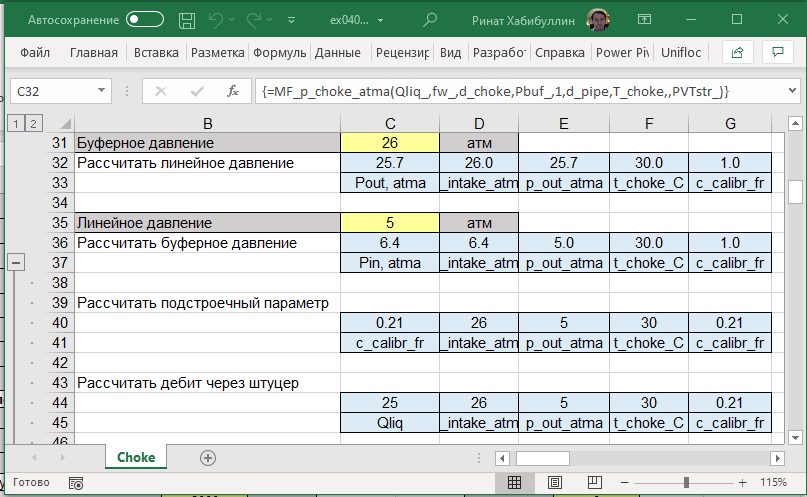
\includegraphics[width=1\linewidth]{choke_array_out}}
	\caption{Пример вывода результата расчета в массив}
	\label{ris:choke_array_out}
\end{figure}


\subsection{MF\_p\_choke\_atma – Расчет давления на входе или на выходе штуцера}
Функция позволяет рассчитать давление на входе или выходе штуцера по известному давлению на противоположном конце при известных параметрах потока (дебите жидкости, обводнённости, газовому фактору). Расчёт проводится по корреляции Перкинса \cite{Perkins_1993} с учётом многофазного потока. 
 
\putlisting{listings/MF_p_choke_atma.lst}



%\subsection{MF\_dp\_choke\_atm – Расчёт перепада давления в штуцере}
%Функция позволяет рассчитать по известному линейному давлению и дебиту или по известному буферному давлению и дебиту перепад давления.  Расчет проводится по корреляции Перкинса \cite{Perkins_1993} с учетом многофазного потока.  
%Функция возвращает перепад давления и температуры в виде массива.
%\putlisting{listings/MF_dp_choke_atm.lst}


\subsection{MF\_qliq\_choke\_sm3day – функция расчёта дебита жидкости через штуцер}
Функция позволяет рассчитать по известному буферному давлению и линейному давлению дебит жидкости. Расчет проводится по корреляции Перкинса \cite{Perkins_1993} с учетом многофазного потока.  

\putlisting{listings/MF_qliq_choke_sm3day.lst}


\subsection{MF\_calibr\_choke\_fr – функция настройки модели штуцера}
Функция позволяет рассчитать корректирующий фактор для модели штуцера, позволяющий согласовать результаты замеров давления и дебита. Расчет проводится по корреляции Перкинса \cite{Perkins_1993} с учетом многофазного потока.  

\putlisting{listings/MF_calibr_choke_fr.lst}

\newpage
\section{Расчет многофазного потока в трубе}

Для расчета участка трубы с использованием пользовательских функций \unf{} применяется схема показанная на рисунке - \ref{ris:Pipe_scheme_1}.

Участок трубы задается как прямой с постоянным наклоном $\theta$  длиной $L$, постоянного диаметра $d$. Поток движется под углом $\theta$ к горизонтальной плоскости. Угол  $\theta$ меняется от -90 до 90 градусов Цельсия. Отрицательная величина  $\theta < 0 $ означает, что поток движется вниз - например отрицательным будет угол наклона для нагнетательной скважины. Следует помнить, что не все гидравлические корреляции поддерживают расчет параметров нисходящего потока (Беггс Брилл работает, для расчета нагнетательных скважин рекомендуется применять эту корреляцию с обводненностью $f_w = 100%$, Ансари только для потока вверх). Угол наклона $\theta = 0 $ соответствует потоку в горизонтальном участке трубопровода.

Труба имеет постоянную по всей длине шероховатость стенок. Шероховатость влияет на коэффициент трения при расчете потока и проявляется при относительно больших скоростях потока. Подробнее про шероховатость и трение в потоке жидкости можно почитать в \cite{Bratland_Pipe_Flow_1}

\begin{figure}[h!]
	\begin{center}
		% https://www.mathcha.io/editor# использован для построения картинок

\tikzset{every picture/.style={line width=0.75pt}} %set default line width to 0.75pt        

\begin{tikzpicture}[x=0.75pt,y=0.75pt,yscale=-1,xscale=1]
%uncomment if require: \path (0,395.3333282470703); %set diagram left start at 0, and has height of 395.3333282470703

%Shape: Can [id:dp2899696286091056] 
\draw  [fill={rgb, 255:red, 250; green, 245; blue, 184 }  ,fill opacity=1 ][line width=2.25]  (164.23,345.91) -- (471.15,94.25) .. controls (473.82,92.06) and (481.92,97.51) .. (489.23,106.43) .. controls (496.54,115.34) and (500.3,124.35) .. (497.63,126.55) -- (190.71,378.2)(164.23,345.91) .. controls (166.9,343.71) and (175,349.16) .. (182.31,358.08) .. controls (189.63,367) and (193.39,376.01) .. (190.71,378.2) .. controls (188.03,380.4) and (179.94,374.95) .. (172.62,366.03) .. controls (165.31,357.11) and (161.55,348.1) .. (164.23,345.91) -- cycle ;
%Shape: Arc [id:dp7673222576415257] 
\draw  [draw opacity=0] (213.54,358.73) .. controls (215.72,361.29) and (217.51,364.25) .. (218.76,367.57) .. controls (220.22,371.43) and (220.84,375.4) .. (220.7,379.27) -- (190.71,378.2) -- cycle ; \draw   (213.54,358.73) .. controls (215.72,361.29) and (217.51,364.25) .. (218.76,367.57) .. controls (220.22,371.43) and (220.84,375.4) .. (220.7,379.27) ;
%Straight Lines [id:da2539925089352497] 
\draw    (111.83,289.33) -- (164.23,345.91) ;


%Straight Lines [id:da27080386920459176] 
\draw    (426.06,41.14) -- (471.15,94.25) ;


%Straight Lines [id:da6784647335940455] 
\draw    (138.03,317.62) -- (448.6,67.7) ;


%Straight Lines [id:da42906958912244875] 
\draw    (343.67,226) -- (373,202.37) ;
\draw [shift={(374.56,201.11)}, rotate = 501.14] [color={rgb, 255:red, 0; green, 0; blue, 0 }  ][line width=0.75]    (10.93,-3.29) .. controls (6.95,-1.4) and (3.31,-0.3) .. (0,0) .. controls (3.31,0.3) and (6.95,1.4) .. (10.93,3.29)   ;

%Straight Lines [id:da31602361859897776] 
\draw    (89,379) -- (569.56,379) ;
\draw [shift={(571.56,379)}, rotate = 180] [color={rgb, 255:red, 0; green, 0; blue, 0 }  ][line width=0.75]    (10.93,-3.29) .. controls (6.95,-1.4) and (3.31,-0.3) .. (0,0) .. controls (3.31,0.3) and (6.95,1.4) .. (10.93,3.29)   ;


% Text Node
\draw (233.67,364.33) node   {$\theta $};
% Text Node
\draw (269.67,187.67) node [rotate=-2.44]  {$L$};
% Text Node
\draw (200.33,343.67) node [rotate=-0.74]  {$P_{in}$};
% Text Node
\draw (472.67,120) node [rotate=-0.74]  {$P_{out}$};
% Text Node
\draw (335.67,230.67) node [rotate=-0.61]  {$Q_{liq}$};


\end{tikzpicture}
		\caption{Схема трубы принятая для расчётов с использованием пользовательских функций}
		\label{ris:Pipe_scheme_1}
	\end{center}
\end{figure}

Для расчёта распределения давления в трубе необходимо задать граничное значение давления на одном из концов трубы. В функциях где где надо задать граничное значение с одного конца трубы оно задается параметром  \mintinline{vb.net}{P_calc_from_atma}. Температура потока в точке, где задается давление, определяется параметром  \mintinline{vb.net}{T_calc_from_C}, температура на другом конце трубы  параметром \mintinline{vb.net}{T_calc_to_C}.  В функциях где надо задать значение давления с двух сторон, используются обозначения \mintinline{vb.net}{P_in_atma} и \mintinline{vb.net}{P_out_atma} соответственно обозначающие давление на стороне где поток входит и выходит. 
Возможно два варианта задания условия - по потоку  \ref{ris:Pipe_scheme_2}  \mintinline{vb.net}{calc_along_flow=1}. и против потока  \ref{ris:Pipe_scheme_3} \mintinline{vb.net}{calc_along_flow=0}. 

\begin{figure}[h!]
	\begin{center}
				\tikzset{every picture/.style={line width=0.75pt}} %set default line width to 0.75pt        
		
		\begin{tikzpicture}[x=0.75pt,y=0.75pt,yscale=-1,xscale=1]
		%uncomment if require: \path (0,390); %set diagram left start at 0, and has height of 390
		
		%Shape: Can [id:dp7382807235009181] 
		\draw  [fill={rgb, 255:red, 250; green, 245; blue, 184 }  ,fill opacity=1 ][line width=2.25]  (176.23,350.28) -- (483.15,98.62) .. controls (485.82,96.43) and (493.92,101.88) .. (501.23,110.8) .. controls (508.54,119.72) and (512.3,128.72) .. (509.63,130.92) -- (202.71,382.57)(176.23,350.28) .. controls (178.9,348.08) and (187,353.54) .. (194.31,362.45) .. controls (201.63,371.37) and (205.39,380.38) .. (202.71,382.57) .. controls (200.03,384.77) and (191.94,379.32) .. (184.62,370.4) .. controls (177.31,361.48) and (173.55,352.47) .. (176.23,350.28) -- cycle ;
		%Shape: Arc [id:dp26711502457409386] 
		\draw  [draw opacity=0] (225.54,363.1) .. controls (227.72,365.66) and (229.51,368.62) .. (230.76,371.95) .. controls (232.22,375.8) and (232.84,379.77) .. (232.7,383.64) -- (202.71,382.57) -- cycle ; \draw   (225.54,363.1) .. controls (227.72,365.66) and (229.51,368.62) .. (230.76,371.95) .. controls (232.22,375.8) and (232.84,379.77) .. (232.7,383.64) ;
		%Straight Lines [id:da2708011557353165] 
		\draw    (123.83,293.7) -- (176.23,350.28) ;
		
		
		%Straight Lines [id:da09547020181005683] 
		\draw    (438.06,45.51) -- (483.15,98.62) ;
		
		
		%Straight Lines [id:da29893852101776] 
		\draw    (150.03,321.99) -- (460.6,72.07) ;
		
		
		%Straight Lines [id:da6573662742713218] 
		\draw    (355.67,230.37) -- (385,206.74) ;
		\draw [shift={(386.56,205.48)}, rotate = 501.14] [color={rgb, 255:red, 0; green, 0; blue, 0 }  ][line width=0.75]    (10.93,-3.29) .. controls (6.95,-1.4) and (3.31,-0.3) .. (0,0) .. controls (3.31,0.3) and (6.95,1.4) .. (10.93,3.29)   ;
		
		%Straight Lines [id:da5485107193914818] 
		\draw    (101,383.37) -- (581.56,383.37) ;
		\draw [shift={(583.56,383.37)}, rotate = 180] [color={rgb, 255:red, 0; green, 0; blue, 0 }  ][line width=0.75]    (10.93,-3.29) .. controls (6.95,-1.4) and (3.31,-0.3) .. (0,0) .. controls (3.31,0.3) and (6.95,1.4) .. (10.93,3.29)   ;
		
		%Right Arrow [id:dp6841435853741948] 
		\draw  [fill={rgb, 255:red, 245; green, 166; blue, 35 }  ,fill opacity=1 ] (135.99,250.8) -- (380.02,50.35) -- (378.16,48.09) -- (395.29,41.6) -- (385.59,57.14) -- (383.73,54.88) -- (139.71,255.32) -- cycle ;
		
		% Text Node
		\draw (245.67,368.7) node   {$\theta $};
		% Text Node
		\draw (281.67,192.04) node [rotate=-2.44]  {$L$};
		% Text Node
		\draw (207.33,354.04) node [rotate=-0.74]  {$P_{in}$};
		% Text Node
		\draw (487.67,117.37) node [rotate=-0.74]  {$P_{out}$};
		% Text Node
		\draw (347.67,235.04) node [rotate=-0.61]  {$Q_{liq}$};
		% Text Node
		\draw  [color={rgb, 255:red, 0; green, 0; blue, 0 }  ,draw opacity=1 ][fill={rgb, 255:red, 245; green, 166; blue, 35 }  ,fill opacity=1 ]  (107, 268.37) circle [x radius= 25.3, y radius= 25.3]   ;
		\draw (107,268.37) node [scale=1.2,rotate=-359.71]  {$P_{calc}$};
		% Text Node
		\draw  [fill={rgb, 255:red, 245; green, 166; blue, 35 }  ,fill opacity=1 ]  (417.67, 24.37) circle [x radius= 23.2, y radius= 23.2]   ;
		\draw (417.67,24.37) node [scale=1.2,rotate=-0.74]  {$P_{out}$};
		
		
		\end{tikzpicture}		
		\caption{Схема расчёта распределения давления по потоку \mintinline{vb.net}{calc_along_flow=1}}
		\label{ris:Pipe_scheme_2}
	\end{center}
\end{figure} 

Схема расчета распределения давления по потоку для случая вертикальной добывающей скважины соответствует расчету распределения давления "снизу вверх" - от забойного давления к устьевому.

\begin{figure}[h!]
	\begin{center}
			
	\tikzset{every picture/.style={line width=0.75pt}} %set default line width to 0.75pt        
	
	\begin{tikzpicture}[x=0.75pt,y=0.75pt,yscale=-1,xscale=1]
	%uncomment if require: \path (0,453); %set diagram left start at 0, and has height of 453
	
	%Shape: Can [id:dp7385102204739014] 
	\draw  [fill={rgb, 255:red, 250; green, 245; blue, 184 }  ,fill opacity=1 ][line width=2.25]  (198.23,370.28) -- (505.15,118.62) .. controls (507.82,116.43) and (515.92,121.88) .. (523.23,130.8) .. controls (530.54,139.72) and (534.3,148.72) .. (531.63,150.92) -- (224.71,402.57)(198.23,370.28) .. controls (200.9,368.08) and (209,373.54) .. (216.31,382.45) .. controls (223.63,391.37) and (227.39,400.38) .. (224.71,402.57) .. controls (222.03,404.77) and (213.94,399.32) .. (206.62,390.4) .. controls (199.31,381.48) and (195.55,372.47) .. (198.23,370.28) -- cycle ;
	%Shape: Arc [id:dp4602786709186524] 
	\draw  [draw opacity=0] (247.54,383.1) .. controls (249.72,385.66) and (251.51,388.62) .. (252.76,391.95) .. controls (254.22,395.8) and (254.84,399.77) .. (254.7,403.64) -- (224.71,402.57) -- cycle ; \draw   (247.54,383.1) .. controls (249.72,385.66) and (251.51,388.62) .. (252.76,391.95) .. controls (254.22,395.8) and (254.84,399.77) .. (254.7,403.64) ;
	%Straight Lines [id:da5353213855148988] 
	\draw    (145.83,313.7) -- (198.23,370.28) ;
	
	
	%Straight Lines [id:da6371642797081225] 
	\draw    (460.06,65.51) -- (505.15,118.62) ;
	
	
	%Straight Lines [id:da5708425902799406] 
	\draw    (172.03,341.99) -- (482.6,92.07) ;
	
	
	%Straight Lines [id:da5694938455522887] 
	\draw    (377.67,250.37) -- (407,226.74) ;
	\draw [shift={(408.56,225.48)}, rotate = 501.14] [color={rgb, 255:red, 0; green, 0; blue, 0 }  ][line width=0.75]    (10.93,-3.29) .. controls (6.95,-1.4) and (3.31,-0.3) .. (0,0) .. controls (3.31,0.3) and (6.95,1.4) .. (10.93,3.29)   ;
	
	%Straight Lines [id:da47656732513988986] 
	\draw    (123,403.37) -- (603.56,403.37) ;
	\draw [shift={(605.56,403.37)}, rotate = 180] [color={rgb, 255:red, 0; green, 0; blue, 0 }  ][line width=0.75]    (10.93,-3.29) .. controls (6.95,-1.4) and (3.31,-0.3) .. (0,0) .. controls (3.31,0.3) and (6.95,1.4) .. (10.93,3.29)   ;
	
	%Right Arrow [id:dp49730840239995544] 
	\draw  [fill={rgb, 255:red, 245; green, 166; blue, 35 }  ,fill opacity=1 ] (419.38,64.16) -- (174.9,264.05) -- (176.75,266.31) -- (159.61,272.77) -- (169.34,257.26) -- (171.19,259.52) -- (415.67,59.63) -- cycle ;
	
	% Text Node
	\draw (267.67,388.7) node   {$\theta $};
	% Text Node
	\draw (303.67,212.04) node [rotate=-2.44]  {$L$};
	% Text Node
	\draw (229.33,374.04) node [rotate=-0.74]  {$P_{in}$};
	% Text Node
	\draw (509.67,137.37) node [rotate=-0.74]  {$P_{out}$};
	% Text Node
	\draw (369.67,255.04) node [rotate=-0.61]  {$Q_{liq}$};
	% Text Node
	\draw  [color={rgb, 255:red, 0; green, 0; blue, 0 }  ,draw opacity=1 ][fill={rgb, 255:red, 245; green, 166; blue, 35 }  ,fill opacity=1 ]  (444, 43.37) circle [x radius= 25.3, y radius= 25.3]   ;
	\draw (444,43.37) node [scale=1.2,rotate=-359.71]  {$P_{calc}$};
	% Text Node
	\draw  [fill={rgb, 255:red, 245; green, 166; blue, 35 }  ,fill opacity=1 ]  (129.67, 288.37) circle [x radius= 21.57, y radius= 21.57]   ;
	\draw (129.67,288.37) node [scale=1.2,rotate=-0.74]  {$P_{in}$};
	
	
	\end{tikzpicture}
		\caption{Схема расчета распределения давления против потока \mintinline{vb.net}{calc_along_flow=0}}
		\label{ris:Pipe_scheme_3}
	\end{center}
\end{figure} 

Схема расчета распределения давления против потока для случая вертикальной добывающей скважины соответствует расчету распределения давления "сверху вниз" - от устьевого давления к забойному.
Все функции для расчета штуцера содержат в названии слово \mintinline{vb.net}{pipe}.

%\subsection{MF\_dp\_pipe\_atm – расчёт перепада давления в трубе}

%Функция позволяет рассчитать перепад давления в участке трубопровода. 
%Функция возвращает давление и температуру в виде массива.

%\putlisting{listings/MF_dp_pipe_atm.lst}

Ниже на рисунке \ref{ris:VLP_curves} приведены результаты расчёта кривой оттока (перепада давления в вертикальной трубе) для различных корреляций, реализованных в \unf{}.

\begin{figure}[h!]
	\begin{center}
	\newcommand{\dPipeDataFile}{data/dPipe.txt}
		\begin{tikzpicture}[scale=1]
		\begin{axis}[
					width=14cm,
					height=10cm,
					xlabel=$Q\; m^3 / day$,
					ylabel=$P_{wf} \; atma$,
					legend pos=south east,
					title=Pipe Pressure Drop]
		\addplot table [y=P_0, x=Q]{\dPipeDataFile};
		\addlegendentry{Beggs Brill}
		\addplot table [y=P_1, x=Q]{\dPipeDataFile};
		\addlegendentry{Ansari}
		\addplot table [y=P_2, x=Q]{\dPipeDataFile};
		\addlegendentry{Unified}
		\addplot table [y=P_3, x=Q]{\dPipeDataFile};
		\addlegendentry{Gray}
		\addplot table [y=P_4, x=Q]{\dPipeDataFile};
		\addlegendentry{Hagedorn Brown}
		\addplot table [y=P_5, x=Q]{\dPipeDataFile};
		\addlegendentry{Sakharov Mokhov}
		\end{axis}
		\end{tikzpicture}	
	\caption{Кривые характеристики многофазного потока для вертикальных труб рассчитанные с использованием различных корреляций }
	\label{ris:VLP_curves}
	\end{center}
\end{figure}

\subsection{MF\_p\_pipe\_atma – функция расчета давления на конце трубы}  
Функция позволяет рассчитать перепад давления в участке трубопровода. Функция обеспечивает несколько режимов расчёта. Некоторые особенности работы функции \mintinline{vb.net}{MF_p_pipe_atma()}
\begin{itemize}
	\item Свойства флюида в трубе определяются параметром \mintinline{vb.net}{str_PVT}, который в свою очередь может быть задан функцией \mintinline{vb.net}{PVT_encode()}.
	\item Дополнительно в поток может быть включен свободный газ. Задается параметром \mintinline{vb.net}{q_gas_sm3day} определяющим объемный расход приведенный к стандартным условиям. Свободный газ суммируется с газом определяемым исходя из заданных свойств флюида. 
	\item Если при определении \mintinline{vb.net}{str_PVT} указан параметр \mintinline{vb.net}{gas_only = 1}, то расчет распределения давления в трубе будет проводиться для газа, наличие жидкости в потоке учитываться не будет. В текущей версии \unf{} при расчете потока газа трение газа не учитывается, перепад давления в газовой линии не зависит от расхода газа, зависит только от плотности газа.
	\item Если параметр дебита жидкости  \mintinline{vb.net}{qliq_sm3day = 0}  равен нулю, расчет проводится для режима барботажа (ZNLF - zero net liquid flow) - движения газа через неподвижный столб жидкости. Расход газа должен быть задан параметром \mintinline{vb.net}{q_gas_sm3day}. В текущей версии \unf{} расчет барботажа проводится проводится за счет переключения на механистическую корреляцию Ансари. Попытка построить график зависимости перепад давления от дебита для других корреляций может дать нелогичный результат около нулевого дебита (скачек перепада давления). Рекомендуется без необходимости для \mintinline{vb.net}{qliq_sm3day = 0} не считать при построении графиков.
	\item Распределение температуры для функции расчета участка скважины ограничено одной моделью - линейного распределения температуры потока вдоль трубы. Для учета температуры необходимо задать параметры \mintinline{vb.net}{t_calc_from_C} и \mintinline{vb.net}{t_calc_to_C} определяющие температуру на концах трубы. В трубе значения будут проинтерполированы по длине. Если второй параметр \mintinline{vb.net}{t_calc_to_C} не задать, то температура в трубе будет постоянной. Проконтролировать расчет температуры можно воспользовавшись выводом результатов расчета в виде массива.
\end{itemize}
 

Результатом работы функций является массив значений содержащий давление и температуру флюида на входе в трубу $P_{in}, T_{in}$, давление и температуру флюида на выходе из трубы $P_{out}, T_{out}$,  калибровочные коэффициент многофазной корреляции для гравитационной составляющей и для трения$c_{calibr\_grav},c_{calibr\_fric}$.  Выходной массив содержит две строки - в первой находятся значения, во второй подписи. Это позволяет при необходимости вывести только значения в той же строке в которой проводился расчет. Значение в первой строке и в первом столбце зависит от настройки функции (параметра \mintinline{vb.net}{calc_along_flow} для функции \mintinline{vb.net}{MF_p_pipe_atma}) и содержит основной результат расчета. Значения в последующих столбцах не зависят от настройки функции и показывают все результаты расчета.
Для вывода массива в Excel следует выбрать необходимый диапазон ячеек, в который будут выводится результаты в виде массива, затем ввести в адресную строку вызов функции и нажать комбинацию клавиш - Cntrl-Shift-Enter. После этого название функции в адресной строке должно отображаться в фигурных скобках, аналогично функции расчета давления в штуцере, рисунок \ref{ris:choke_array_out}. При необходимости внести коррективы в вызов функции также необходимо подтверждать свои действия комбинацией клавиш Cntrl-Shift-Enter.

\putlisting{listings/MF_p_pipe_atma.lst}

\subsection{MF\_calibr\_pipe - функция калибровки расчета участка трубы}

Функция калибровки позволяет настроить модель потока в трубе под замеры давления на концах трубы. Настройка может проводиться за счет подбора различных параметров. В текущей реализации может быть подобран только один из перечисленных ниже параметров.
\begin{itemize}
	\item Калибровочный коэффициент многофазной корреляции для гравитационной составляющей  $c_{calibr\_grav}$. Ищется в диапазоне от 0.5 до 1.5.
	\item Калибровочный коэффициент многофазной корреляции для трения $c_{calibr\_fric}$. Ищется в диапазоне от 0.5 до 1.5.
	\item Газовый фактор $R_p$. Ищется в диапазоне $[0.5 R_p, 2 R_p]$ относительно заданного газового фактора. 
	\item Обводненность $f_w$.  Ищется в диапазоне $[0.5 f_w, 2 f_w]$ относительно заданной обводненности. 
\end{itemize}

\putlisting{listings/MF_calibr_pipe.lst}

%\subsection{MF\_p\_pipe\_znlf\_atma – функция расчета давления на конце трубы при барботаже}  
% отдельной функции для барботажа больше нет - если дебит задать ноль то и MF_p_pipe_atma будет считать барботаж
%
%\putlisting{listings/MF_p_pipe_znlf_atma.lst}

\subsection{MF\_dpdl\_atmm – функция расчета градиента давления по многофазной корреляции}  

\putlisting{listings/MF_dpdl_atmm.lst}

\newpage

        % Глава многофазный поток
%	
\section{Расчет многофазного потока в пласте}
Для анализа работы скважины и скважинного оборудования в большинстве случаев достаточно простейшего подхода для описания производительности пласта. На текущий момент в \unf{} используется линейная индикаторная кривая с поправкой Вогеля для учета разгазирования в призабойной зоне пласта с учетом обводненности \cite{KBrown_AL_methods_vol4}. 

Пользовательские функции для расчета производительности пласта начинаются с префикса  \mintinline{vb.net}{IPR_}. 

Для расчета притока из пласта необходимо определить связь между дебитом жидкости $Q_{liq}$ (притоком) и забойным давлением работающей скважины $P_{wf}$.
Линейная индикаторная кривая на основе закона Дарси задает такую связь через коэффициент продуктивности скважины, который определяется как 
\begin{equation}\label{PI_def} 
 PI = \frac{Q_{liq}}{P_{res} - P_{wf}} 
\end{equation}

где $P_{res}$ - пластовое давление - давление на контуре питания скважины. Закон Дарси описывает установившийся приток несжимаемой жидкости в однородном пласте. 

Соответственно уравнение притока будет иметь вид

$$ Q_{liq} = PI \left( P_{res} - P_{wf} \right) $$

Для линейного притока по закону Дарси коэффициент продуктивности может быть оценен либо по данным эксплуатации из уравнения \ref{PI_def} либо по аналитической зависимости по характеристикам пласта и системы заканчивания. Например для радиального притока к вертикальной скважине широко известна формула Дюпюи согласно которой 
\begin{equation}\label{eq_Dupui} 
PI = f \cdot \frac{kh}{\mu B}\frac{1}{ \ln \dfrac{r_e}{r_w} + S }  
\end{equation}

здесь $f$ - размерный коэффициент, зависящий от выбранной системы единиц для остальных параметров. Так для системы единиц

\newcommand{\rnttab}[1]{
	\begin{tabular}[c]{@{}c@{}}#1\end{tabular}	
}

\begin{table}[]
	\centering
	\caption{Размерности параметров выражения \ref{eq_Dupui}} \label{tab:dim_Dupui}
	\begin{tabular}{|c|c|c|c|c|}
		\hline
		Обозначение & Параметр   			        	& СИ           & \rnttab{Практические \\ метрические}     & \rnttab{Американские\\ промысловые} \\ \hline
		$f$        & \rnttab{размерный \\ коэффициент} & $2\pi$       & $\dfrac{1}{18.41}$     			      & $\dfrac{1}{141.2}$                      \\ \hline
		$k$        & проницаемость           		    & $\text{м}^2$ & мД                    					  & mD   							    \\ \hline
		$h$        & \rnttab{мощность \\ пласта}       & м            & м                      				  & ft   								    \\ \hline		
		$B$        & \rnttab{объемный \\ коэффициент}  & $\text{м}^3/\text{м}^3$    & $\text{м}^3/\text{м}^3$    & $scf/bbl$    						\\ \hline
		$\mu$      & вязкость                           & Па $\cdot$ с & сП                                       & сP                                  \\ \hline
		$r_e$      & \rnttab{радиус зоны \\ дренирования} & м & м                                       & ft                                  \\ \hline
		$r_w$      & \rnttab{радиус  \\ скважины} & м & м                                       & ft                                  \\ \hline
		$S$        & скин фактор 				   & \multicolumn{3}{c|}{безразмерный}                     \\ \hline
	\end{tabular}
\end{table}
 
 При снижении забойного давления добывающей скважины ниже давления насыщения, выражение оценка дебита жидкости по закону Дарси  оказывается завышенной. Газ выделяющийся в призабойной зоне пласта создает дополнительное гидравлическое сопротивление.  В \unf поправка на снижение забойного давления ниже давления насыщения реализована на основе поправки Вогеля. Для безводной нефти по Вогелю продуктивности скважины по данным тестовой эксплуатации - дебите жидкости $Q_{liq}$ и соответствующем забойном давлении $P_{wf}$ может быть оценен по выражению \ref{eq_Vogel}.
 
 \begin{equation}\label{eq_Vogel} 
 PI = \frac{Q_{liq}}{P_{res} - P_{b} + \dfrac{P_{b}}{1.8} \left[ 1.0 - 0.2  \dfrac{P_{wf}}{P_{b}}- 0.8 \left( \dfrac{P_{wf}}{P_{b}} \right)^2 \right] }   
 \end{equation}
 
 При наличии обводненности зависимость усложняется.
 
 В \unf реализована модель определения коэффициента продуктивности по данным эксплуатации. Сравнение индикаторных кривых, построенных по тестовым данным $Q_{liq} = 100$ и $P_{wf} = 150$ при наличии и отсутствии воды приведено на рисунке. 
 
 \newcommand{\dPipeDataFile}{data/IPR_fw_data.txt}
 \begin{tikzpicture}[scale=1]
 \begin{axis}[
 width=14cm,
 height=10cm,
 xlabel=$Q\; m^3 / day$,
 ylabel=$P_{wf} \; atma$,
 legend pos=north east,
 title=Pipe Pressure Drop]
 \addplot table [y=Pwf_fw0, x=Q_fw0]{\dPipeDataFile};
 \addlegendentry{$f_w = 0$}
 \addplot table [y=Pwf_fw95, x=Q_fw95]{\dPipeDataFile};
\addlegendentry{$f_w = 95$}
 \end{axis}
 \end{tikzpicture}
 
 

\subsection{IPR\_pi\_sm3dayatm – расчёт продуктивности}
Функция позволяет рассчитать коэффициент продуктивности скважины по данным тестовой эксплуатации. Особенность линейной модели притока к скважине с поправкой Волегя заключается в минимальном наборе исходных данных, необходимых для построения индикаторной кривой. Достаточно знать пластовое давление и дебит и забойное давление в одной точке.

\putlisting{listings/IPR_pi_sm3dayatm.lst}


\subsection{IPR\_pwf\_atm – расчёт забойного давления по дебиту и продуктивности}
Функция позволяет рассчитать забойное давление скважины по известным значениям дебита и продуктивности.

\putlisting{listings/IPR_pwf_atma.lst}

\subsection{IPR\_qliq\_sm3day – расчёт дебита по забойному давлению и продуктивности}
Функция позволяет рассчитать дебит жидкости скважины на поверхности по забойному давлению и продуктивности.

\putlisting{listings/IPR_qliq_sm3day.lst}



\newpage
       % Глава индикаторная кривая
%	\section{Расчет УЭЦН}
Пользовательские функции, связанные с расчетом установок электрических центробежных насосов приведены в модуле «u7\_Excel\_functions\_ESP».  Названия функций начинаются с префикса ESP. 

УЭЦН состоит из следующих основных конструктивных элементов:
\begin{itemize}
	\item ЦН - центробежный насос. Модуль обеспечивающий перекачку жидкости за счет преобразования механической энергии вращения вала в гидравлическую мощность. 
	\item ПЭД - погружной электрический двигатель. Модуль обеспечивающий преобразование электрической энергии, поступающей по кабелю к погружному электрическому двигателю в механическую энергию вращения вала.
	\item ГС - газосепаратор или приемный модуль. Модуль обеспечивающий забор пластовой жидкости из скважины и подачу ее в насос. При этом центробежный газосепаратор способен отделить часть свободного газа в потоке и направить его в межтрубное пространство скважины. Работает за счет механической энергии вращения вала.
	\item вал - узел передающий энергию от погружного электрического двигателя (ПЭД) к остальным узлам установки, в том числе к центробежному насосу.
	\item кабель - узел передающий электрическую энергию с поверхности к погружному электрическому двигателю
	\item трансформатор - узел обеспечивающий необходимое напряжение на кабеле на поверхности. Как правило на вход трансформатора подается напряжение 380 В, а на выходе оно поднимается до нескольких тысяч вольт. 
	\item СУ - станция управления ЭЦН. Узел управляющий работой системы УЭЦН. Может запускать и  останавливать скважины, обеспечивает защиту установки ЭЦН при нежелательных режимах работы
	\item ЧРП - частотно регулируемый привод. Обычно комплектуется со станцией управления УЭЦН. Обеспечивает изменение частоты колебаний напряжения и тока, а соответственно и частоты вращения вала ЭЦН. Может отсутствовать в компоновке УЭЦН. 
\end{itemize}

В промысловых сводках и отчетах часто ЭЦН обозначаются с использованием значений габарита насоса, номинальной подачи и номинального напора. ЭЦН5А 50 - 2000, означает что, это насос 5А габарита, с номинальной подачей 50 м3/сут и напором 2000 м. 

\begin{figure}[h!]
	\center{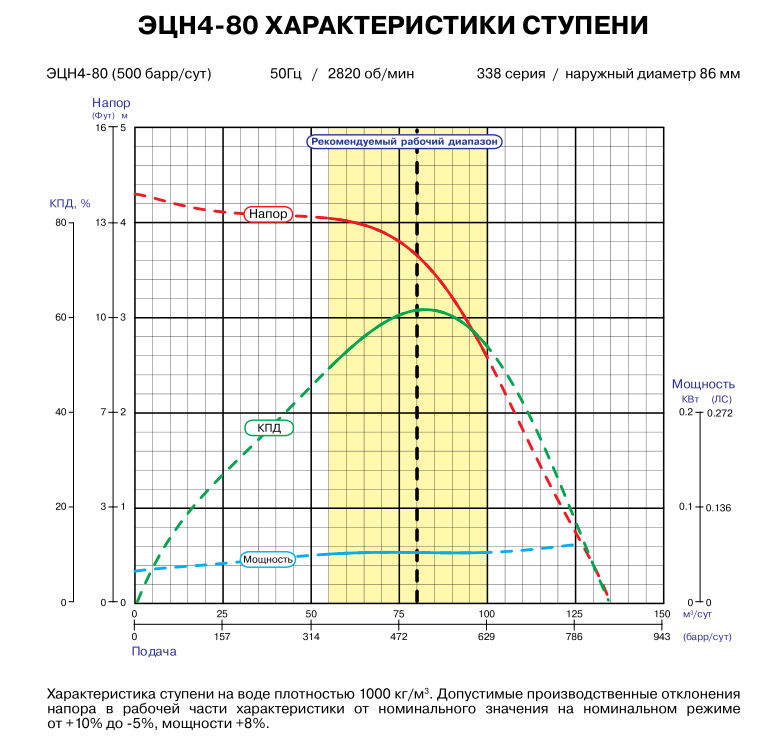
\includegraphics[width=0.8\linewidth]{novomet_ESP_80}}
	\caption{Пример каталожных характеристик ЭЦН}
	\label{ris:novomet_ESP_80}
\end{figure}

УЭЦН, как и другие центробежные машины, обладает относительно узким диапазоном подач при которых достигается достаточно высокий КПД его работы (от 30 до 60\%). В связи с этим для различных подач выпускаются различные типы УЭЦН. Всего в промышленности используются сотни различных типов ЭЦН различных производителей. Характеристики различных насосов предоставляются производителями в каталогах оборудования и обычно встраиваются в расчетные программы в виде баз данных характеристик оборудования. В надстройке \unf{} содержится база данных характеристик ЭЦН, которая может быть использована при проведении расчетов пользовательскими функциями. База сокращенная, содержит ряд насосов только одного производителя. Как правило этого достаточно для проведения базовых расчетов, так как характеристики насосов одного типоразмера разных производителей схожи между собой. 

Для выбора определенного насоса из базы необходимо использовать его идентификатор в базе - \mintinline{vb.net}{pump_id}

Задача расчета УЭЦН обычно сводится к следующим:
\begin{itemize}
	\item Прямая задача - по заданным значениям дебита жидкости скважины,  давлению на приеме, напряжению питания УЭЦН на поверхности найти давление на выкиде насоса, потребляемую электрическую мощность, потребляемый ток установки, КПД всей системы и отдельных узлов системы
	\item Обратная задача - по данным контроля параметров работы УЭЦН на поверхности - потребляемому току, напряжению питания частоте подаваемого напряжения, данным по конструкции УЭЦН и скважины найти дебит жидкости и обводнённость по скважине, давление на приеме и забойное давление.
	\item Задача узлового анализа - по данным конструкции скважины, параметров работы погружного оборудования оценить дебит по жидкости скважины при заданным параметрах работы УЭЦН или при их изменении. К этому типу задач относится задача подбора погружного оборудования для достижения заданных условий эксплуатации 
	
\end{itemize}

Для расчёта УЭЦН требуется рассчитать гидравлические параметры работы ЦН и электромеханические параметры ПЭД.

\subsection{ESP\_head\_m – расчёт номинального напора ЭЦН}
Функция позволяет получить паспортные характеристики ЭЦН - напор при определенной подаче. 

\putlisting{listings/ESP_head_m.lst}

Расчет выполняется на основе паспортных характеристик ЦН. 

\subsection{ESP\_eff\_fr – расчёт номинального КПД ЭЦН}
Функция позволяет получить паспортные характеристики ЭЦН - КПД  при определенной подаче. 

\putlisting{listings/ESP_eff_fr.lst}

Расчет выполняется на основе паспортных характеристик ЦН. 

\subsection{ESP\_power\_W – расчёт номинальной мощности потребляемой ЭЦН}
Функция позволяет получить паспортные характеристики ЭЦН - мощность, потребляемую с вала при определенной подаче. 

\putlisting{listings/ESP_power_W.lst}

Расчет выполняется на основе паспортных характеристик ЦН. 

\subsection{ESP\_id\_by\_rate – выбор типового насоса по номинальному дебиту}
Функция возвращает идентификатор типового насоса по заданному номинальному дебиту. 
Может быть использована для выбора насоса на основе его наименования типа ЭЦН 50 - 2000.
\putlisting{listings/ESP_id_by_rate.lst}

\subsection{ESP\_dp\_atm – расчет перепада давления развиваемого ЭЦН}
Функция рассчитывает перепад давления, развиваемый ЦН при заданных параметрах флюида и термобарических условиях.
\putlisting{listings/ESP_dp_atm.lst}

\subsection{ESP\_system\_calc – расчет параметров работы УЭЦН}
Функция рассчитывает полный набор параметров работы УЭЦН при заданных параметрах флюида и термобарических условиях. В отличии от функции  \mintinline{vb.net}{ESP\_dp\_atm} учитывает проскальзывание при расчете частоты вращения вала и рассчитываются электические параметры работы ЭЦН
\putlisting{listings/ESP_system_calc.lst}


\subsection{Электромеханический расчёт погружного электрического двигателя ПЭД}
Рассматривается асинхронный электрический двигатель. 

Погружные асинхронные электрические двигатели для добычи нефти выполяются трехфазными. 

Впервые конструкция трёхфазного асинхронного двигателя была разработана, создана и опробована русским инженером М. О. Доливо-Добровольским в 1889-91 годах. Демонстрация первых двигателей состоялась на Международной электротехнической выставке во Франкфурте на Майне в сентябре 1891 года. На выставке было представлено три трёхфазных двигателя разной мощности. Самый мощный из них имел мощность 1.5 кВт и использовался для приведения во вращение генератора постоянного тока. Конструкция асинхронного двигателя, предложенная Доливо-Добровольским, оказалась очень удачной и является основным видом конструкции этих двигателей до настоящего времени.

За прошедшие годы асинхронные двигатели нашли очень широкое применение в различных отраслях промышленности и сельского хозяйства. Их используют в электроприводе металлорежущих станков, подъёмно-транспортных машин, транспортёров, насосов, вентиляторов. Маломощные двигатели используются в устройствах автоматики.

Широкое применение асинхронных двигателей объясняется их достоинствами по сравнению с другими двигателями: высокая надёжность, возможность работы непосредственно от сети переменного тока, простота обслуживания.

Для расчёта электромеханических параметров погружных электрических двигателей полезно понимать теоретические основы их работы. Теория работы погружных асинхронных двигателей не отличается от теории применимой к двигателям применяемым на поверхности. Далее кратко изложены основные положения теории. 

Трехфазная цепь является частным случаем многофазных систем электрических цепей, представляющих собой совокупность электрических цепей, в которых действуют синусоидальные ЭДС одинаковой частоты, отличающиеся по фазе одна от другой и создаваемые общим источником энергии.
Переменный ток, протекающий по трехфазной цели, характеризуется следующими параметрами:

\begin{itemize}
	\item Фазное напряжение $U_A, U_B, U_C $ - напряжение между линейным проводом и нейтралью
	\item Линейное напряжение $U_{AB}, U_{BC}, U_{CA} $ - напряжение между одноименными выводами разных фаз
	\item Фазный ток $I_{phase}$ – ток в фазах двигателя.
	\item Линейный ток $I_{line}$ – ток в линейных проводах.
	\item $ \cos \varphi $ - коэффициент мощности, где $ \varphi$ величина сдвига по фазе между напряжением и током 
\end{itemize}

Подключение двигателя к цепи трехфазного тока может быть выполнено по схеме "звезда"\ или "треугольник".

\begin{figure}[h!]
	\center{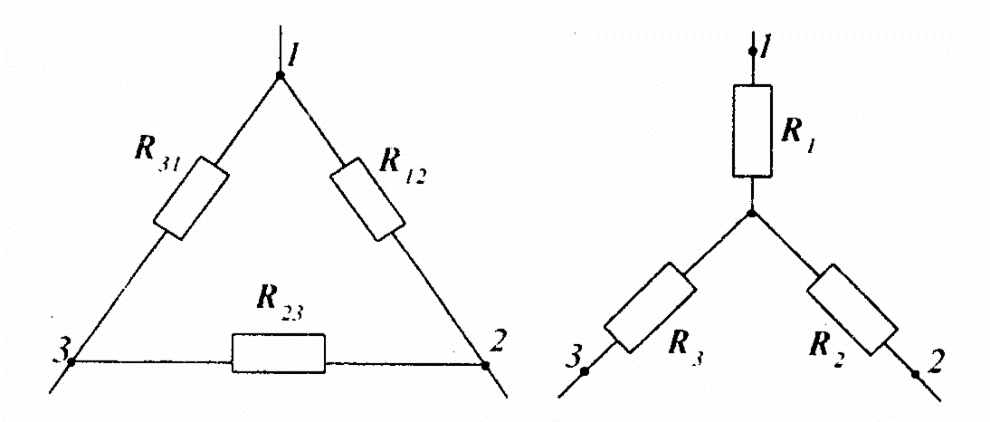
\includegraphics[width=1\linewidth]{electicity_triangle_star}}
	\caption{Пример схем замещения: \"треугольник\" и \"звезда\"}
	\label{ris:electicity_triangle_star}
\end{figure}

Для схемы звезда фазное напряжение меньше линейного в $\sqrt{3}$ раз.

$$ U_{AB} = \sqrt{3} U_{A} $$
$$ I_{phase} = I_{line} $$

Для схемы треугольник 

$$ U_{AB} =  U_{A} $$
$$ I_{line} =\sqrt{3} I_{phase} $$


В погружных двигателях обычно применяет схема подключения звезда. Эта схема обеспечивает более низкое напряжение в линии, что способствует повышению КПД передачи энергии по длинному кабелю. Еще есть причины?
При схеме подключения звезда токи в линии и в фазной обмотке статора двигателя совпадают, поэтому значение тока обозначают $I$ не указывая индекс в явном виде. Поскольку линейное напряжения проще измерить и легче контролировать параметры трехфазного двигателя обычно задаются линейными. В частности номинальное напряжение питания двигателя это линейное напряжение (напряжение между фазами). Далее линейное напряжение будет обозначать без индекса как $U$

Активная электрическая мощность в трехфазной цепи задается выражением 
$$ P= \sqrt{3}U I \cos \varphi$$

Реактивная мощность 
$$ Q= \sqrt{3}U I \sin \varphi$$

Соответственно полная мощность 
$$ S= \sqrt{3}U I $$

\subsubsection{ Устройство трёхфазной асинхронной машины}
Неподвижная часть машины называется статор, подвижная – ротор. Обмотка статора состоит из трёх отдельных частей, называемых фазами.

При подаче переменного напряжения и тока на обмотки статора внутри статора формируется вращающееся магнитное поле. Частота вращения магнитного поля совпадает с частотой питающего напряжения. 

Магнитный поток $\Phi $ и напряжение подаваемое на статор связаны приближенным соотношением 
$$ U_1 \approx E_1 = 4.44 w_1 k_1 f \Phi $$
где 

 $\Phi$ -  магнитный поток;
 
 $U_1$ -	напряжение в одной фазе статора;
 
 $f$   - частота сети;
 
 $E_1$	- ЭЦН в фазе статора;
 
 $w_1$ - число витков одной фазы обмотки статора;
 
 $k_1$  - обмоточный коэффициент.
   
Из этого выражения следует, что магнитный поток $\Phi $ в асинхронной машине не зависит от её режима работы, а при заданной частоте сети $f$ зависит только от действующего значения приложенного напряжения $U_1$


Для ЭДС ротора можно записать выражение 


$$  E_2 = 4.44 w_2 k_2 f S \Phi $$

где 


$S$ - величина скольжения (проскальзывания);

$E_2$	- ЭЦН в фазе ротора;

$w_2$ - число витков одной фазы обмотки ротора;

$k_2$ - обмоточный коэффициент ротора.

ЭДС, наводимая в обмотке ротора, изменяется пропорционально скольжению и в режиме двигателя имеет наибольшее значение в момент пуска в ход.
Для тока ротора в общем случае можно получить такое соотношение

$$  I_2 = \frac{E_2 S}{\sqrt{R_2^2+(S X_2^2)}} $$

где 

$R_2$ -  активное сопротивление обмотки ротора, связанное с потерями на нагрев обмотки;  

$X_2 = 2 \pi f L_2$ - индуктивное сопротивление обмотки неподвижного ротора, связанное с потоком рассеяния;

Отсюда следует, что ток ротора зависит от скольжения и возрастает при его увеличении, но медленнее, чем ЭДС.

Для асинхронного двигателя можно получить следующее выражение для механического момента 

$$ M = \frac{1}{4.44 w_2 k_2 k_T^2 f} \frac{U_1^2 R_2 S}{R_2^2 + (S X_2^2)^2}$$

где 

$k_T = \frac{E_1}{E_2} = \frac{w_1 k_1}{w_2 k_2}$ - коэффициент трансформации асинхронной машины

Из полученного выражения для электромагнитного момента следует, что он сильно зависит от подведённого напряжения ($M \sim U_1^2$). При снижении, например, напряжения на 10\%, электромагнитный момент снизится на 19\% $M \sim (0,9U_1)^2=0.81 U_1^2)$. Это является одним из недостатков асинхронных двигателей. 

Электромеханическая модель погружного АПЭД реализована в расчетных функциях \unf{} как модель двигателя с номером 0  \mintinline{vb.net}{motorID = 0}

Функции для расчета характеристик ПЭД начинаются с префикса \mintinline{vb.net}{motor_}. Описание функций можно найти в приложении "Автоматически сгенерированное описание".

\subsubsection{Каталожные характеристики АПЭД}

\begin{figure}[h!]
	\center{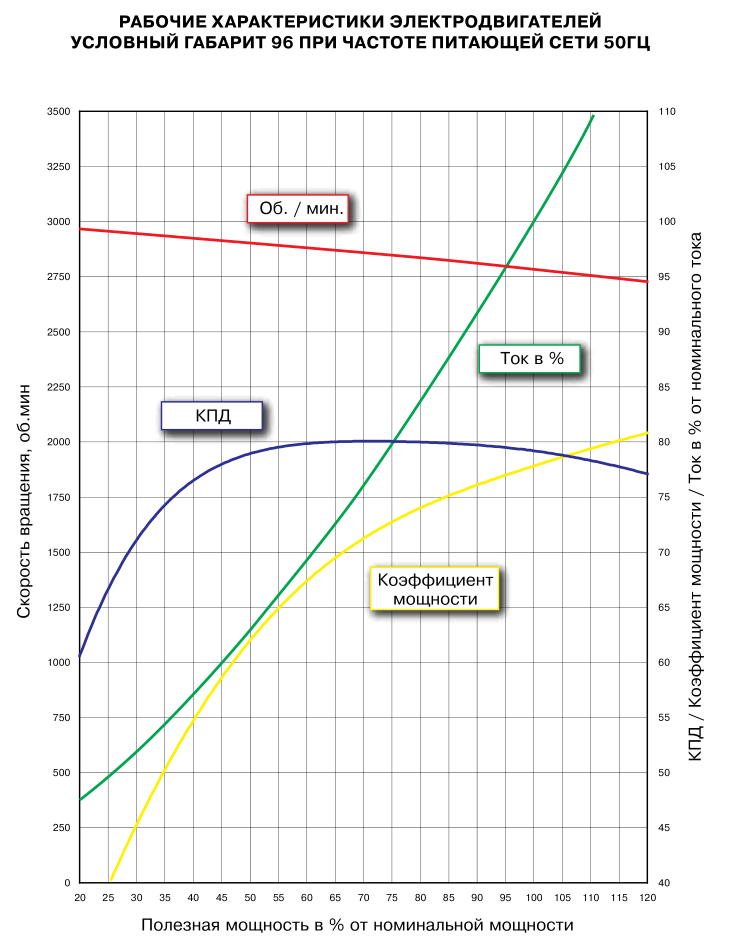
\includegraphics[width=0.6\linewidth]{novomet_motor_1}}
	\caption{Каталожные характеристики ПЭД}
	\label{ris:novomet_motor_1}
\end{figure}

Для асинхронных погружных двигателей производители в каталогах оборудования приводят характеристики, позволяющие оценить КПД, потребляемый ток, частоту вращения вала и коэффициент электрической мощности от загрузки для определенной частоты вращения - рисунок \ref{ris:novomet_motor_1}. Нередко характеристики приводятся для двух частот вращения - 50Гц и 60 Гц.


Каталожная модель погружного АПЭД реализована в расчетных функциях \unf как модель двигателя с номером 1  \mintinline{vb.net}{motorID = 1}

Функции для расчета характеристик ПЭД начинаются с префикса \mintinline{vb.net}{motor_}. Описание функций можно найти в приложении "Автоматически сгенерированное описание".



\newpage
           % Глава ЭЦН
%	

\section{Технологический режим добывающих скважин}
Одна из первых реализаций расчётных модулей \unf{} была создана для проведения расчётов потенциала добычи нефти в форме технологического режима добывающих скважин. Расчёты были реализованы в начале 2000х годов. Расчётная форма оказалась удобной для практического применения и со временем алгоритмы расчёта распространились по разным компаниям и широко использовались.

Функции расчета параметров технологического режима добывающих скважин находятся в модуле «tr\_mdlTecRegimes»

Для обеспечения обратной совместимости расчётов в \unf{} заложены основные функции расчёта из технологического режима работы скважин. У функций изменены названия функций и имена аргументов, однако алгоритмы расчётов оставлены без изменений.

Пользовательские функции для расчета параметров технологического режима работы добывающих скважин начинаются с префикса  \mintinline{vb.net}{tr_}. 

\newpage
\subsection{tr\_Pwf\_calc\_atma – расчёт забойного давления по динамическому уровню}

Функция рассчитывает забойное давление добывающей нефтяной скважины. Расчёт выполняется по известному значению затрубного давления и динамическому уровню. \cite{Khasanov_TR_2006}

Результат расчёта - абсолютное значение забойного давления. 

Расчёт выполняется по модифицированной корреляции Хасана-Кабира оптимизированной для скорости вычисления как для интервала выше насоса в межтрубном пространстве, так и для участка ниже насоса. При расчёте пренебрегается трением в потоке и используются упрощённые PVT зависимости, что позволило получить результат в аналитическом виде и ускорить расчёты. [ссылку надо будет привести когда то] 

Функция позволяет учесть удлинения скважин для забоя, глубины спуска насоса, и динамического уровня. Два последних значения являются опциональными и могут быть опущены при проведении расчёта. 

%\putlisting{listings/tr_Pwf.txt}



\subsection{tr\_Pwf\_calc\_Pin\_atma – расчёт забойного давления по давлению на приеме}
Функция рассчитывает забойное давление добывающей нефтяной скважины по известному значению давления на приёме насоса. 

Результат расчёта - абсолютное значение забойного давления. 

Расчёт выполняется по модифицированной корреляции Хасана-Кабира оптимизированной для скорости вычисления для участка ниже насоса. При расчёте пренебрегается трением в потоке и используются упрощённые PVT зависимости, что позволило получить результат в аналитическом виде и ускорить расчёты. [ссылку надо будет привести когда то] 

Функция позволяет учесть удлинения скважин для забоя, глубины спуска насоса. Последние значения являются опциональными и могут быть опущены при проведении расчёта. 
%\putlisting{listings/tr_Pwf_calc_Pin_atma.txt}


\subsection{tr\_Ppump\_calc\_atma – расчёт давления на приеме по динамическому уровню}
Функция рассчитывает давление на приёме насоса добывающей нефтяной скважины по известному значению затрубного давления и динамическому уровню. 

Расчёт выполняется по модифицированной корреляции Хасана-Кабира оптимизированной для скорости вычисления для участка выше насоса. При расчёте пренебрегается трением в потоке и используются упрощённые PVT зависимости, что позволило получить результат в аналитическом виде и ускорить расчёты. [ссылку надо будет привести когда то]. Значение коэффициента сепарации используется для оценки объёмного расхода газа в межтрубном пространстве. 

Результат расчёта - абсолютное значение давления на приёме насоса. 
%\putlisting{listings/tr_Ppump_calc_atma.txt}



\subsection{tr\_Potential\_Pwf\_atma – расчёт целевого забойного давления по доле газа}
Функция рассчитывает целевое забойное давление добывающей нефтяной скважины, при котором достигается заданная доля газа в потоке.

Результат расчёта - абсолютное значение забойного давления. 
%\putlisting{listings/tr_Potential_Pwf_atma.txt}

\subsection{tr\_BB\_Pwf\_atma – расчёт забойного давления фонтанирующей скважины по буферному давлению}
Функция рассчитывает забойное давление фонтанирующей добывающей скважины по известному значению буферного давления. Расчет выполняется по корреляции Бегсса Брилла. 

Расчет отличается рядом упрощений - из PVT свойств используется только значение газового фактора - давление насыщения и объемный коэффициент газа вычисляются по корреляциям. 

В отличии от расчёта скважин с насосом в корреляции Беггса Брилла учитывается наличие трения. Хотя для низких дебитов эта корреляция может давать завышенные значения перепада давления. 

Для расчётов рекомендуется использовать функцию \unf{} реализующую аналогичную функциональность с меньшим набором допущений

Результат расчёта - абсолютное значение забойного давления. 
%\putlisting{listings/tr_BB_Pwf_atma.vb}

\subsection{tr\_BB\_Pwf\_Pin\_atma – расчёт забойного давления по давлению на приеме по корреляции Беггса-Брилла}
Функция рассчитывает забойное давление  добывающей скважины по известному значению давления на приёме. Расчёт выполняется по корреляции Бегсса-Брилла. 
Расчёт отличается рядом упрощений - из PVT свойств используется только значение газового фактора - давление насыщения и объёмный коэффициент газа вычисляются по корреляциям. 

В отличии от расчёта скважин с насосом в корреляции Беггса Брилла учитывается наличие трения. Хотя для низких дебитов эта корреляция может давать завышенные значения перепада давления. 

Для расчётов рекомендуется использовать функцию \unf{} реализующую аналогичную функциональность с меньшим набором допущений

Результат расчёта - абсолютное значение забойного давления. 

%\putlisting{listings/tr_BB_Pwf_Pin_atma.vb}

           % Глава тех режим
	\chapter{Упражнения по работе с пользовательскими функциями \unf}

Освоить работу с расчетными функциями \unf можно выполняя упражнения описанные в данном разделе и изучая устройство тестовых расчетных модулей. Упражнение демонстрируют некоторые подходы к использованию \unf. На основе этих подходов можно создать свои расчетные модули решающие специфические задачи пользователя. 

\section{Расчет PVT свойств}

Расчет физико химических свойств пластовых флюидов лежит в основе всех расчетов систем нефтедобычи. При решении прикладных задач редко возникает необходимость расчета PVT свойств непосредственно, однако понимание принципа их расчета, а особенно зависимости результатов расчета от исходных данных важно.
	
Цель упражнений по расчету PVT свойств:
\begin{itemize}	
	\item 	освоить принципы работы c пользовательскими функций \unf 
	\item 	изучить влияние исходных PVT данных на результаты расчета PVT свойств
	\item 	изучить влияние выбора PVT корреляций на результаты расчета PVT свойств
	\item 	изучить механизм калибровки PVT корреляций на результаты измерений
\end{itemize}
	 
	 
\subsection{Построение простых PVT зависимостей}

Для выполнения упражнения используйте файл "10.PVT.xlsx"

\begin{enumerate}
	\item Запустите файл с надстройкой \unf. Для того чтобы убедиться, что надстройка запущена откройте редактор VBE (Alt+F11). В дереве проектов должен отображаться файл надстройки \mintinline{vb.net}{UniflocVBA_7.xlam}, рис. \ref{ris:VBE_empty}.
	
	\begin{figure}[h!]
		\center{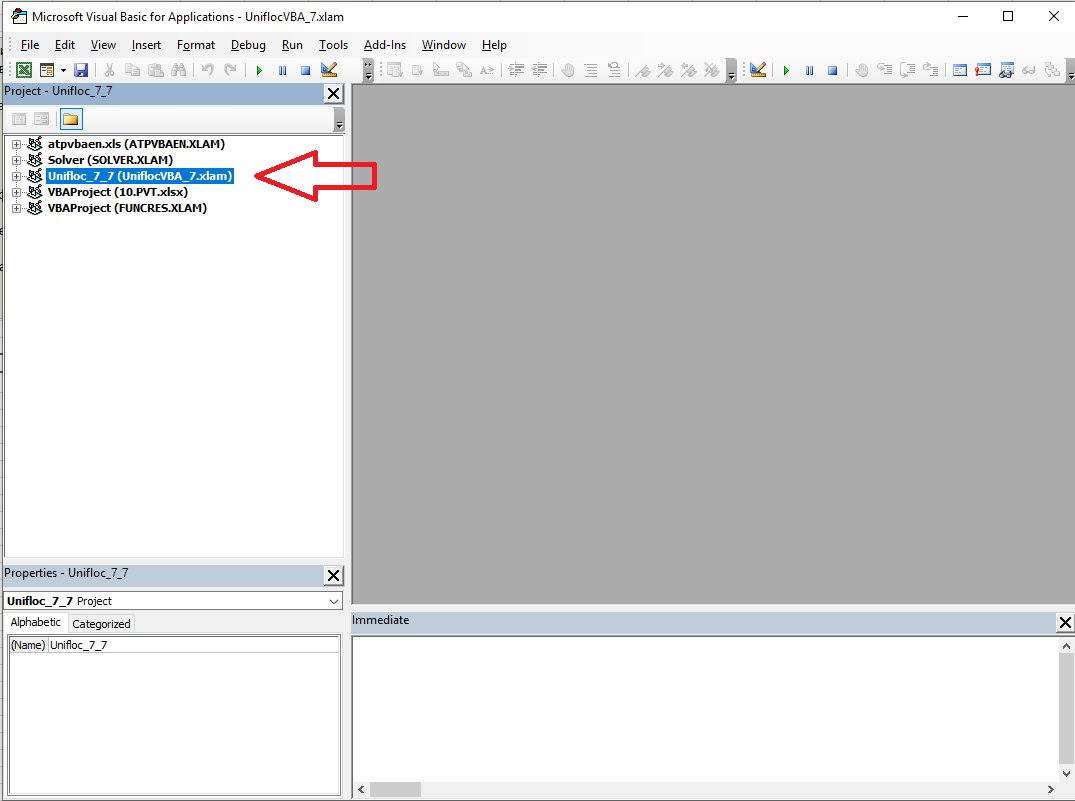
\includegraphics[width=0.5\linewidth]{VBE_empty}}
		\caption{Окно редактора VBE с загруженной надстройкой \unf}
		\label{ris:VBE_empty}
	\end{figure}

	\item Откройте файл с упражнением \texttt{10.PVT.xlsx} (смотри рис. \ref{ris:Ex10_1}).
	
	\begin{figure}[h!]
		\center{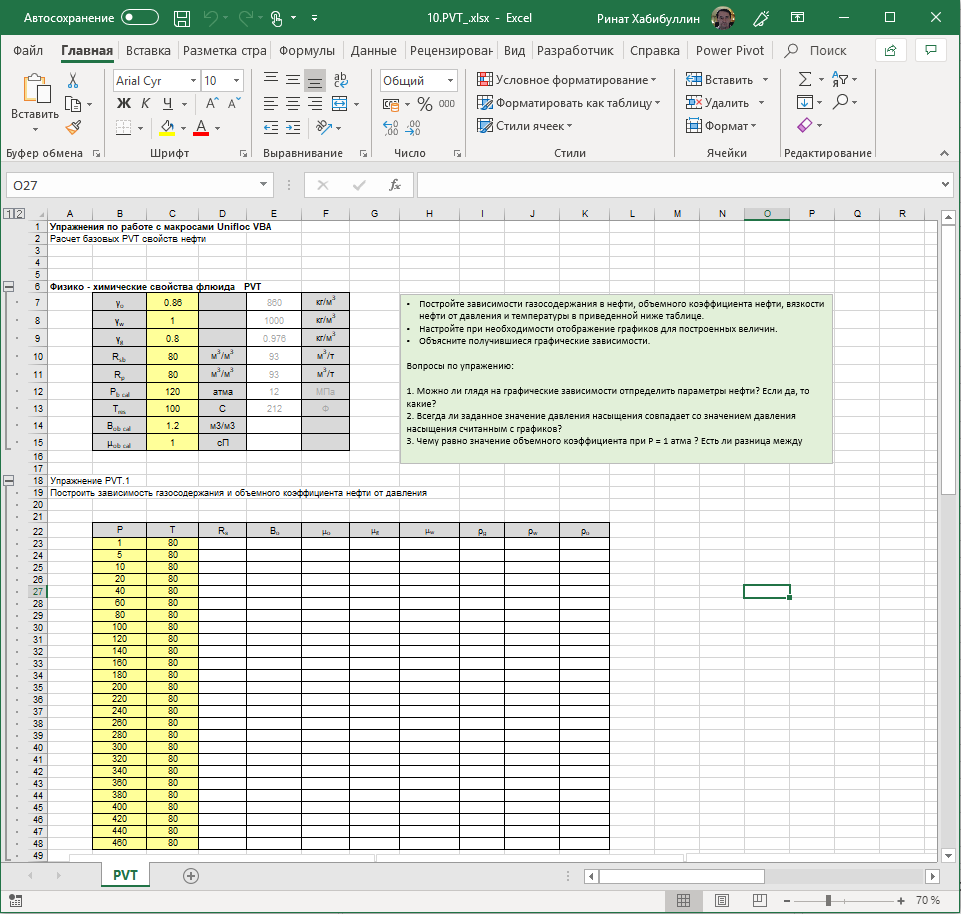
\includegraphics[width=0.5\linewidth]{Ex10_1}}
		\caption{Открытый файл с упражнением \texttt{10.PVT.xlsx}}
		\label{ris:Ex10_1}
	\end{figure}
	
	\item Для расчета первого элемента таблицы в ячейках D23:D48 - газосодержания в нефти при давлении 1 атм и температуре 80 °C - введите в ячейку D23 строку
	
	{ \small  \texttt{=PVT\_Rs\_m3m3(B23;C23;gamma\_gas\_;gamma\_oil\_; gamma\_wat\_; Rsb\_; Rp\_; Pb\_; Tres\_; Bob\_; muob\_)}}
	
	Обратите внимание -- при запущенной надстройке достаточно начать вводить в ячейку формулу, например ввести \texttt{=PVT} как Excel откроет выпадающий список с подсказкой, показывающий возможные варианты названий функций (смотри рис. \ref{ris:Ex10_2}). 
	
	В приведенной строке \texttt{B23;C23} - ссылки на соответствующие ячейки,  \texttt{gamma\_gas\_;gamma\_oil\_} - также ссылки на ячейки, которые предварительно были поименованы. 

	\begin{figure}[h!]
		\center{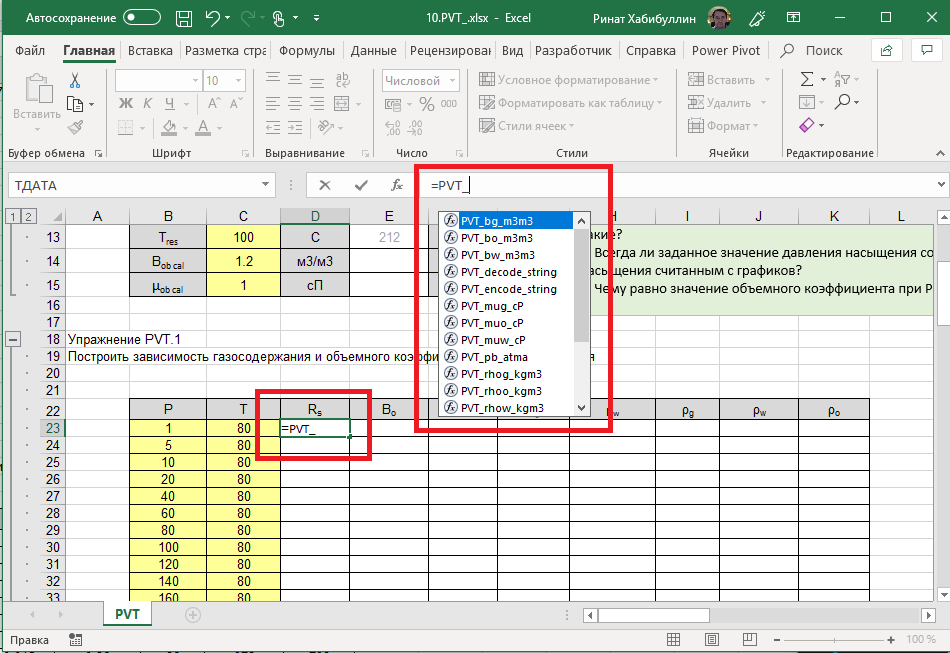
\includegraphics[width=0.5\linewidth]{Ex10_2}}
		\caption{Выпадающий список с подсказками названий функции}
		\label{ris:Ex10_2}
	\end{figure}

	Из выпадающего списка выберите функцию \texttt{=PVT\_Rs\_m3m3(} после чего нажмите кнопку $f_x$ "вставить функцию" слева от строки формул. Это вызовет окно задания параметров функции, в котором будут указаны все параметры, которые необходимо ввести. В этом окно можно ввести необходимые значения параметров или указать ссылки на соответствующие ячейки.

	\begin{figure}[h!]
		\center{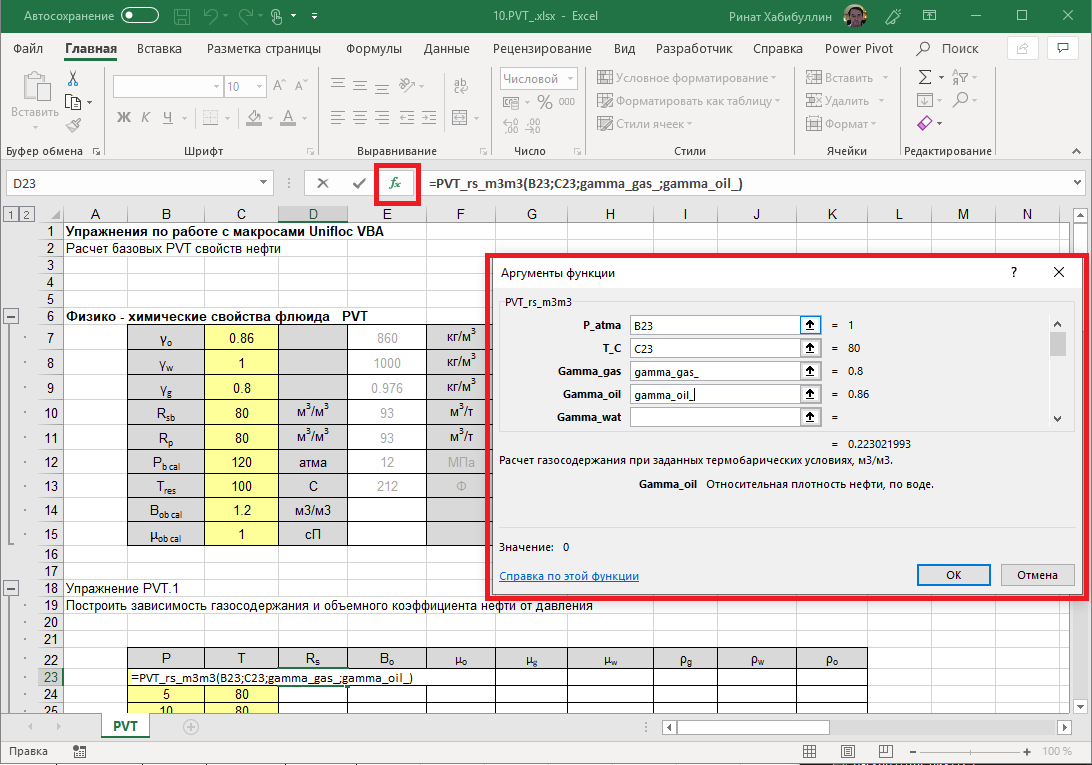
\includegraphics[width=0.5\linewidth]{Ex10_3}}
		\caption{Окно ввода аргументов функции}
		\label{ris:Ex10_3}
	\end{figure}

	\item После ввода всех параметров и нажатия кнопки ОК в ячейке должен отобразиться результат расчета. Воспользовавшись инструментом "Влияющие ячейки" на вкладке "Формулы" можно отследить на какие ячейки ссылается введенная формула
	\begin{figure}[h!]
		\center{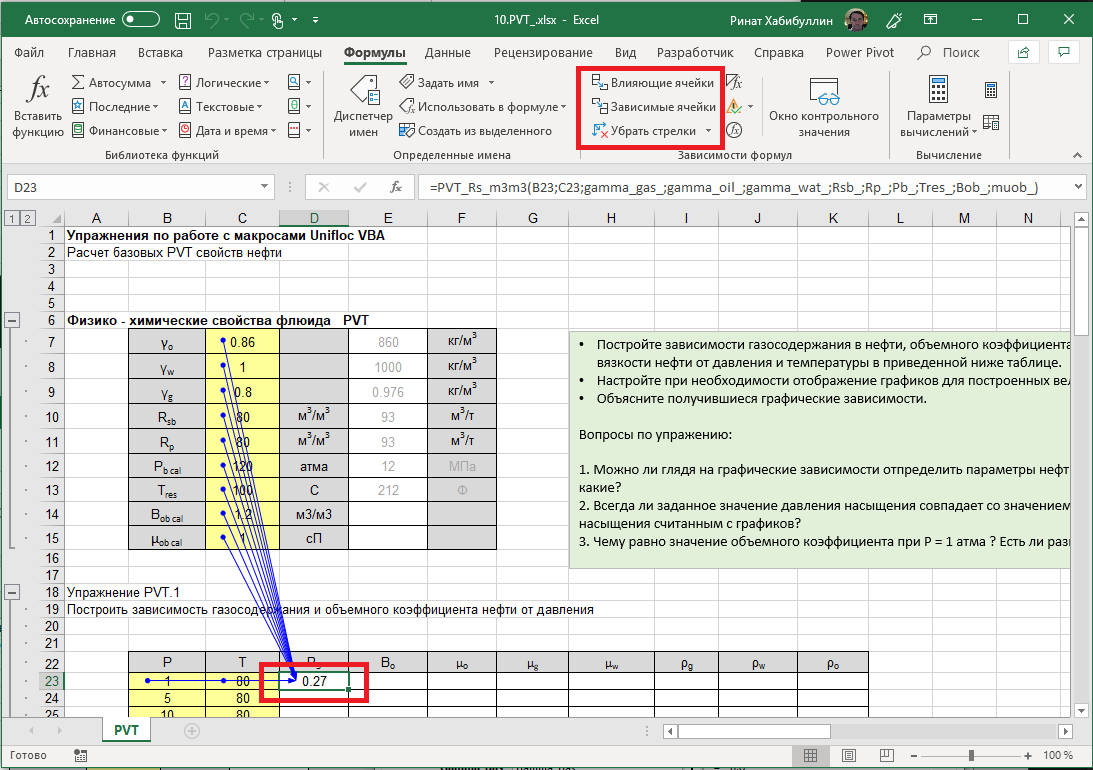
\includegraphics[width=0.5\linewidth]{Ex10_4}}
		\caption{Результат вызова пользовательской функции с отображение влияющих ячеек}
		\label{ris:Ex10_4}
	\end{figure}

	\item Аналогично заполните все ячейки таблицы  \texttt{D23:D48} вызовами функции \texttt{=PVT\_Rs\_m3m3()} с соответствующими параметрами. Это можно сделать "протянув" ранее введенную функцию в ячейке \texttt{D23}.
	
	Обратите внимание, что при "протягивании" поименованные ячейки оказываются закрепленными, а ссылки на значения давления и температуры съезжают вместе с протягиваемой ячейкой. Результат показан на рисунке \ref{ris:Ex10_5}
	\begin{figure}[h!]
		\center{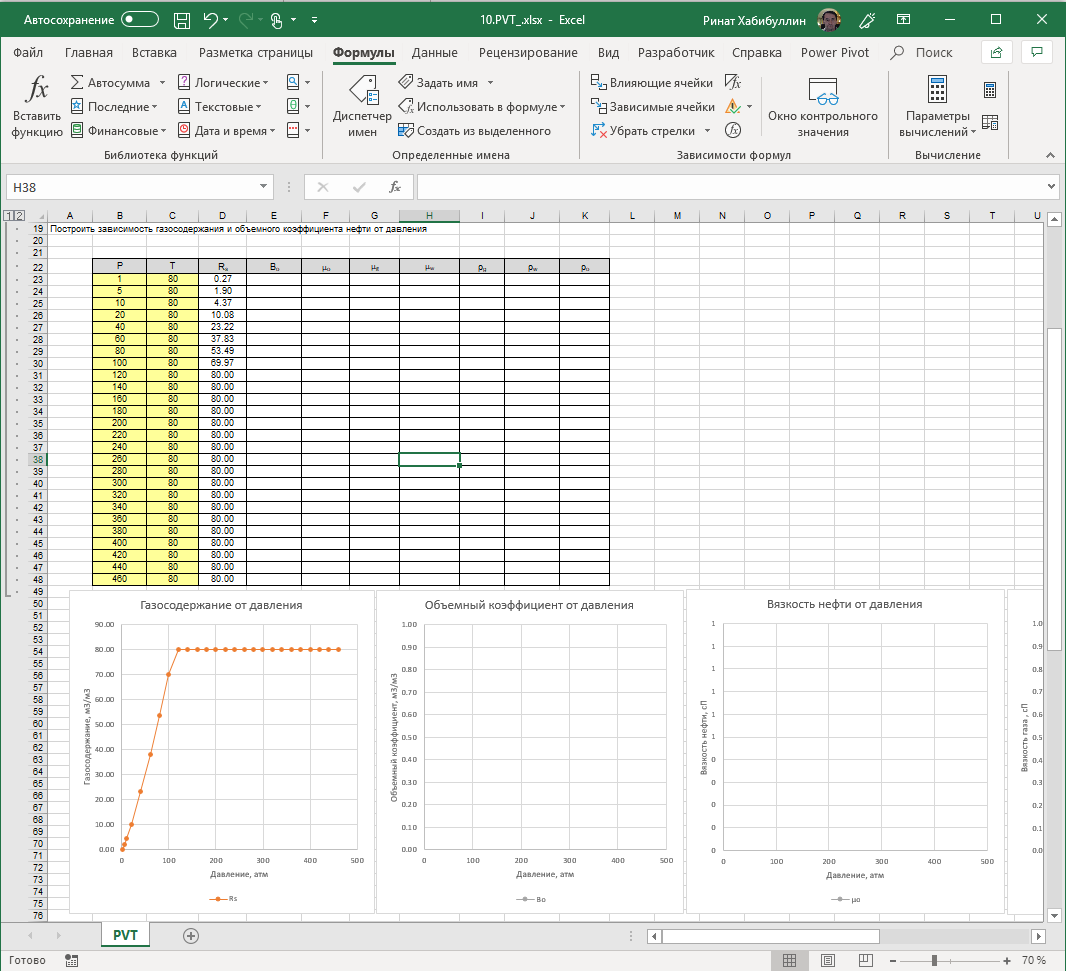
\includegraphics[width=0.5\linewidth]{Ex10_5}}
		\caption{Результат расчета зависимости газосодержания от давления}
		\label{ris:Ex10_5}
	\end{figure}

	\item По аналогии с зависимостью газосодержания от давления постройте графики зависимости других параметров от давления. Используйте следующие функции для проведения расчатов: 
	
	функция расчета объемного коэффициента нефти
	
	{ \small  \texttt{=PVT\_Bo\_m3m3(B23;C23;gamma\_gas\_;gamma\_oil\_;gamma\_wat\_; Rsb\_; Rp\_; Pb\_;Tres\_;Bob\_;muob\_)}}
	
	функция расчета вязкости нефти при заданных термобарических условиях
	
	{ \small  \texttt{=PVT\_Muo\_cP(B23;C23;gamma\_gas\_;gamma\_oil\_;gamma\_wat\_; Rsb\_; Rp\_; Pb\_;Tres\_;Bob\_;muob\_)}}
	
    функция расчета вязкости газа при заданных термобарических условиях
	
	{ \small  \texttt{=PVT\_Mug\_cP(B23;C23;gamma\_gas\_;gamma\_oil\_;gamma\_wat\_; Rsb\_; Rp\_; Pb\_;Pb\_;Bob\_;muob\_)}}
	
	функция расчета вязкости воды при заданных термобарических условиях
	
	{ \small  \texttt{=PVT\_Muw\_cP(B23;C23;gamma\_gas\_;gamma\_oil\_;gamma\_wat\_; Rsb\_; Rp\_; Pb\_;Tres\_;Bob\_;muob\_)}}
	
	функция расчета плотности газа при заданных термобарических условиях
	
	{ \small  \texttt{=PVT\_Rhog\_kgm3(B23;C23;gamma\_gas\_;gamma\_oil\_;gamma\_wat\_; Rsb\_; Rp\_; Pb\_;Tres\_;Bob\_;muob\_)}}
	
	функция расчета плотности воды при заданных термобарических условиях
	
	{ \small  \texttt{=PVT\_Rhow\_kgm3(B23;C23;gamma\_gas\_;gamma\_oil\_;gamma\_wat\_; Rsb\_; Rp\_; Pb\_;Tres\_;Bob\_;muob\_)}}
	
	функция расчета плотности нефти при заданных термобарических условиях
	
	{ \small  \texttt{=PVT\_Rhoo\_kgm3(B23;C23;gamma\_gas\_;gamma\_oil\_;gamma\_wat\_; Rsb\_; Rp\_; Pb\_;Tres\_;Bob\_;muob\_)}}
	
	Результаты приведены на рисунке \ref{ris:Ex10_6}
	
	\begin{figure}[h!]
		\center{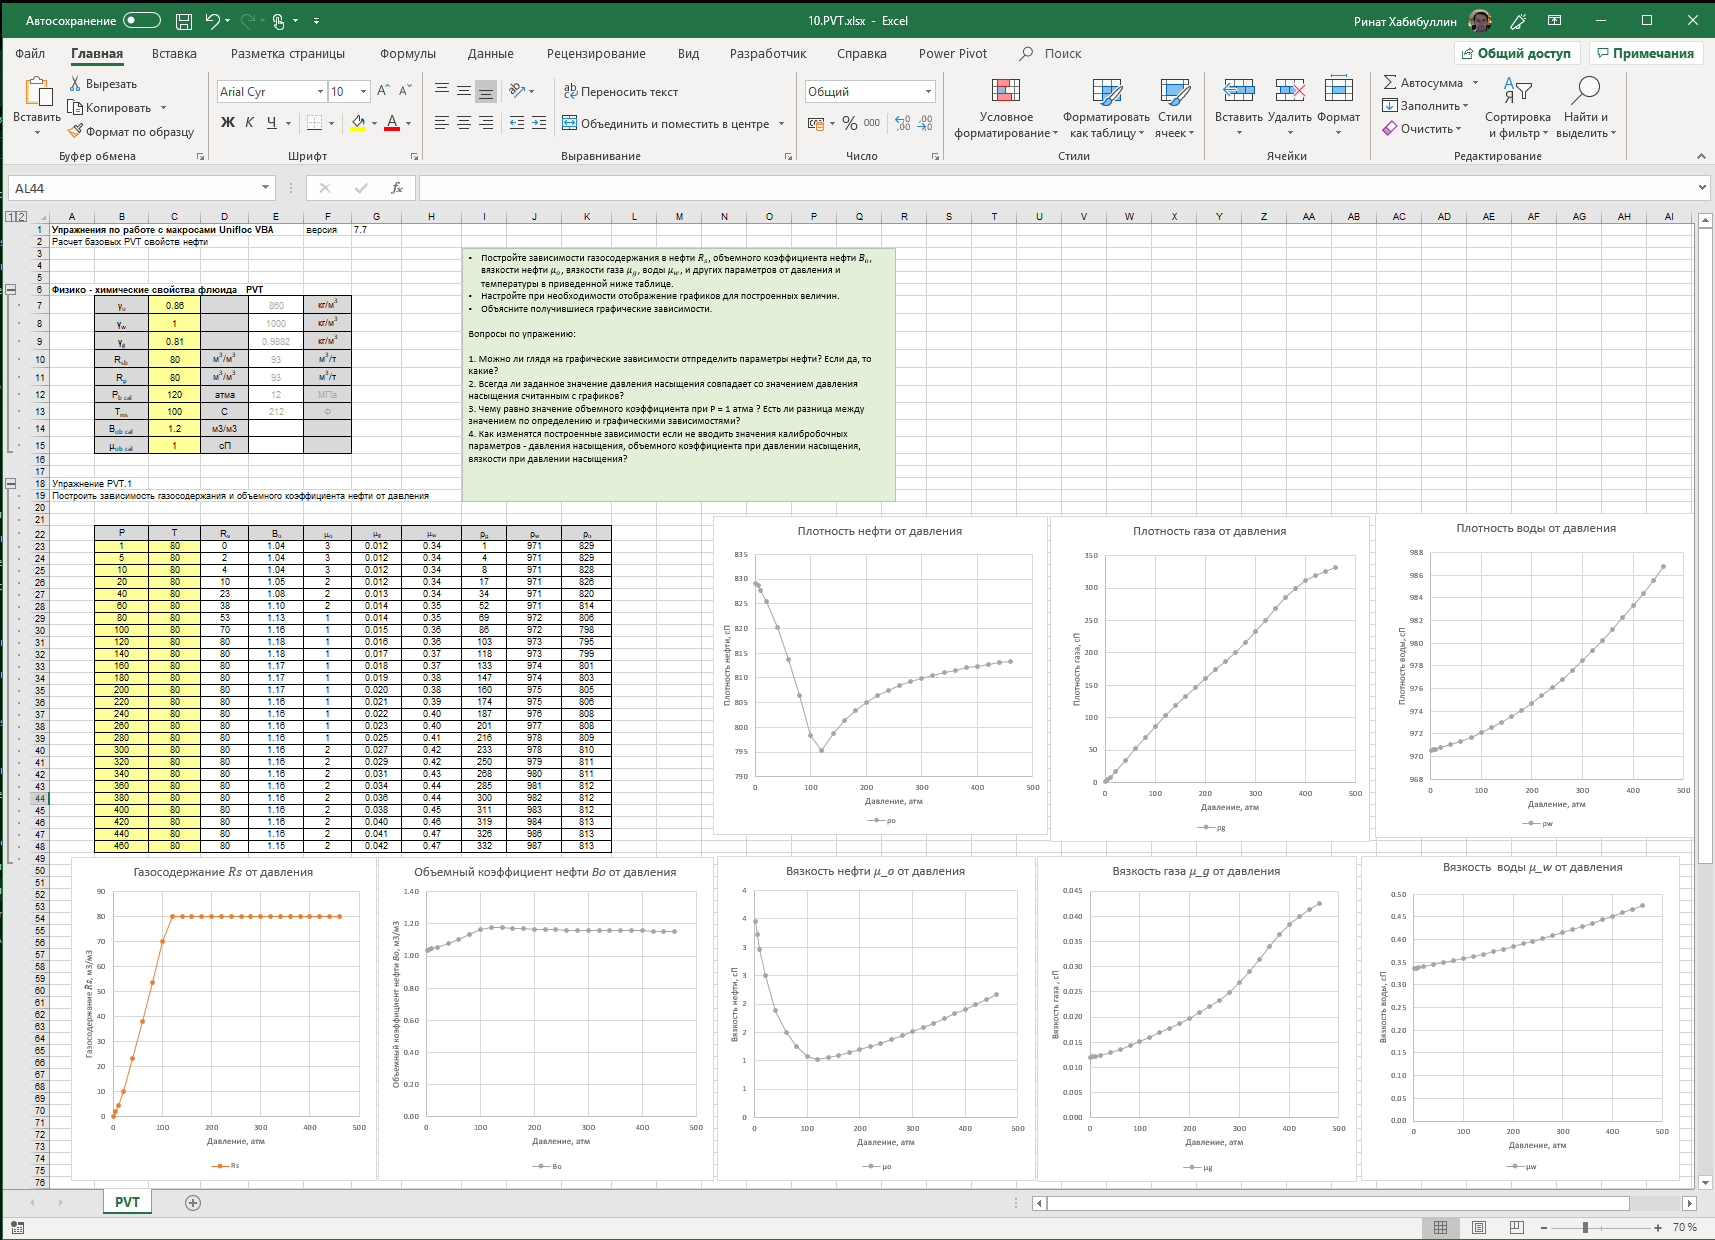
\includegraphics[width=1\linewidth]{Ex10_6}}
		\caption{Результат расчета зависимости свойств пластовых флюидов от давления}
		\label{ris:Ex10_6}
	\end{figure}
	
	\item Ответьте на вопросы по упражнению приведенные в рабочей книге.
	
	\begin{enumerate}
		\item Можно ли глядя на графические зависимости определить параметры нефти? Если да, то какие?
		\item Всегда ли заданное значение давления насыщения совпадает со значением давления насыщения считанным с графиков?
		\item Чему равно значение объемного коэффициента при Р = 1 атма? Есть ли разница между исходным значением и значением определенным по графическими зависимостями?
		\item Как изменятся построенные зависимости если не вводить значения калибровочных параметров - давления насыщения, объемного коэффициента при давлении насыщения, вязкости при давлении насыщения?
		
	\end{enumerate}
 
\end{enumerate}

\section{Расчет производительности скважины}

Модель притока к скважине является достаточно простой и одновременно полезной, позволяя оперативно оценивать добычные возможности скважины. Для индикаторной диаграммы Вогеля зависимость забойного давления от дебита ниже давления насыщения перестает быть линейной.

Для выполнения упражнения необходимо задать:
\begin{enumerate}
	\item PVT свойства флюидов
	\item Параметры работы скважины на установившемся режиме
	\item Пластовое давление
\end{enumerate}


\begin{figure}[h!]
	\center{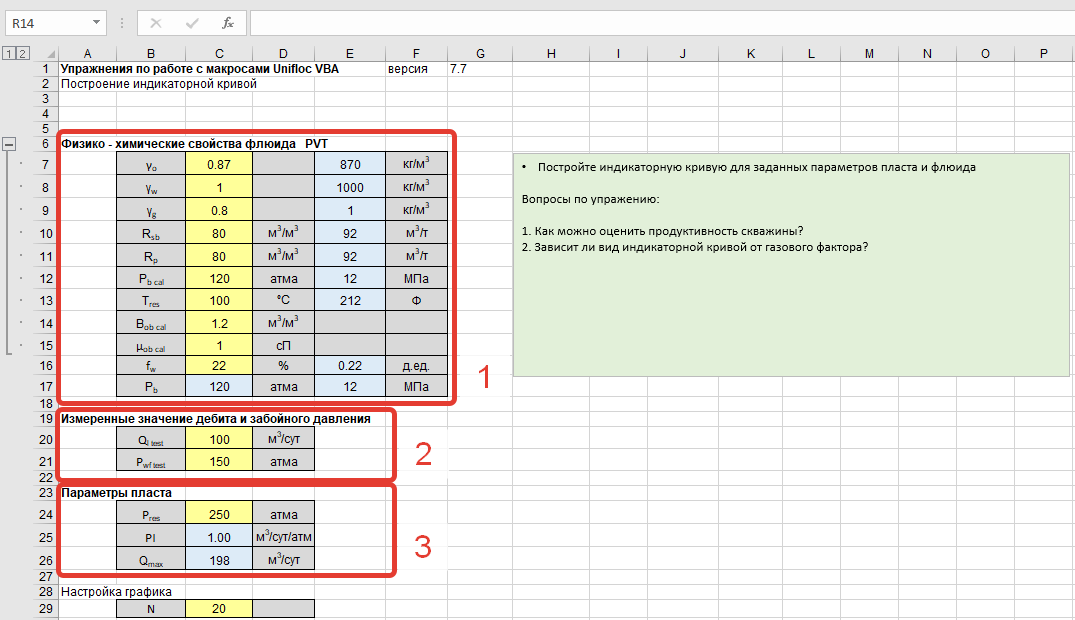
\includegraphics[width=1\linewidth]{Ex20_1}}
	\caption{Исходные данные для построения индикаторной кривой}
	\label{ris:Ex20_1}
\end{figure}

Коэффициент продуктивности $PI$ скважины рассчитывается в ячейке С25 по замеренным данным  с помощью функции

{ \small  \texttt{=IPR\_PI\_sm3dayatm(qltest\_;Pwftest\_;Pres\_;fw\_;Pb\_)}}

А максимальный дебит $Q_{max}$ при максимальной депрессии с забойным давлением равном нулю

{ \small  \texttt{=IPR\_Qliq\_sm3Day(PI\_;Pres\_;0;fw\_;Pb\_)}}

После задания всех необходимых параметров перейдем к построению индикаторной кривой.

Для расчета забойного давления в зависимости от дебита введите в ячейку D40 строку

{ \small  \texttt{=IPR\_Pwf\_atma(PI\_;Pres\_;C40;fw\_;Pb\_)}}

Для вычисления дебита в зависимости от давления Вы можете воспользоваться функцией 

{ \small  \texttt{=IPR\_Qliq\_sm3Day(PI\_;Pres\_;D40;fw\_;Pb\_)}}

поместив ее в ячейку E40.

\begin{figure}[h!]
	\center{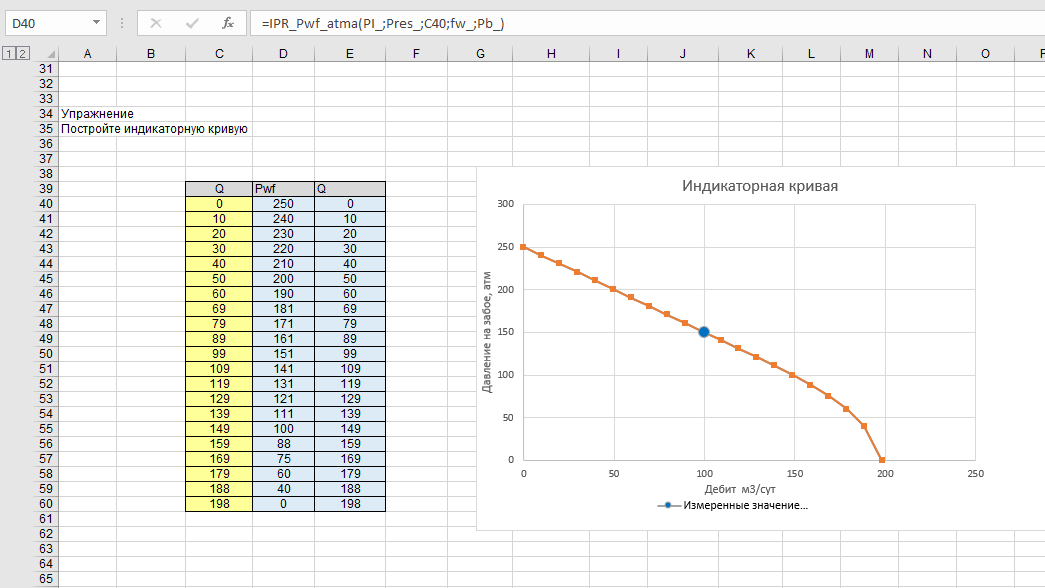
\includegraphics[width=1\linewidth]{Ex20_2}}
	\caption{Результат построения индикаторной кривой}
	\label{ris:Ex20_2}
\end{figure}

Применяя функции, строя дополнительные графики, ответьте на вопросы по упражнению, приведенные в рабочей книге.

	\begin{enumerate}
		\item Как можно оценить продуктивность скважины?
		\item Зависит ли вид индикаторной кривой от газового фактора?
	\end{enumerate}

\section{Набор расчетных модулей анализа скважины}
Пример использования алгоритмов \unf   приведен в файле \texttt{UF7\_calc\_well.xlsm}.

Файл содержит набор расчетных модулей позволяющих провести анализ данных описывающих работу скважины с применением различных методов добычи.


\subsection{Расчетный модуль анализа и настройки PVT свойств}

 % Глава описание упражнений
%	\chapter*{Заключение}                       % Заголовок

Заключение возможно будет тут когда то      % Заключение
%	\chapter*{Единицы измерений} % Заголовок
\addcontentsline{toc}{chapter}{Единицы измерений}  % Добавляем его в оглавление
\noindent

\section*{Давление}
 
 atm, атм "--- физическая атмосфера 
 
 atma, атма "--- абсолютное значение величины в атмосферах
 
 atmg, атми "--- избыточное (измеренное) значение величины в атмосферах. отличается от абсолютной на величину атмосферного давления (1.01325 атма)

\chapter*{Список сокращений и условных обозначений} % Заголовок
\addcontentsline{toc}{chapter}{Список сокращений и условных обозначений}  % Добавляем его в оглавление
\noindent

$\gamma_g$  - \mintinline{vb.net}{gamma_gas} - удельная плотность газа, по воздуху. 

$\gamma_o$  - \mintinline{vb.net}{gamma_oil} - удельная плотность нефти, по воде.

$\gamma_w$  - \mintinline{vb.net}{gamma_wat}- удельная плотность воды, по воде. 

$R_{sb}$ - \mintinline{vb.net}{Rsb_m3m3} газосодержание при давлении насыщения, м3/м3. 

$R_p$ - \mintinline{vb.net}{Rp_m3m3}. замерной газовый фактор, м3/м3.

$P_b$ - \mintinline{vb.net}{Pb_atma}. давление насыщения, атма.  

$T_{res}$ - \mintinline{vb.net}{Tres_C} пластовая температура, \textcelsius. 

$B_{ob}$ - \mintinline{vb.net}{Bob_m3m3} объёмный коэффициент нефти, м3/м3. 

$\mu_{ob}$ - \mintinline{vb.net}{Muob_cP}. вязкость нефти при давлении насыщения, сП. 

$Q_{liq}$ - \mintinline{vb.net}{Qliq_scm3day}. дебит жидкости измеренный на поверхности (приведенный к стандартным условиям), м3/сут. 

$f_{w}$ - \mintinline{vb.net}{fw_perc, fw_fr} объёмная обводненность (fraction of water), проценты или доли единиц. 

$PI$ - \mintinline{vb.net}{pi_sm3dayatm} - коэффициент продуктивности скважины, м3/сут/атм
        % Список сокращений и условных обозначений
	\chapter*{Словарь терминов}             % Заголовок
\addcontentsline{toc}{chapter}{Словарь терминов}  % Добавляем его в оглавление

Словарь описывает термины и сокращения широко используемые в описании и в системе \unf.


\textbf{VBA} "--- Visual Basic for Application язык программрования встроенный в Excel и использованный для написания макросов \unf.

\textbf{VBE} "--- Среда разработки для языка VBA. Встроена в Excel.

\textbf{BHP, Pwf} "--- Bottom hole pressure. Well flowing pressure Забойное давление

\textbf{BHT, TBH} "--- Bottom hole temperature. Забойная температура

\textbf{WHP, PWH} "--- Well head pressure. Устьевое давление. Как правило, соответствует буферному давлению.

\textbf{WHT, TWH} "--- Well head temperature. Устьевая температура. Температура флюида на устье скважины. Температура в точке замера буферного давления.

\textbf{IPR} "--- Inflow performance relationship. Индикаторная кривая. Зависимость забойного давления от дебита для пласта. Широко используется в узловом анализе.

\textbf{VLP, VFP} "--- Vertical lift performance, vertical flow performance, outflow curve. Кривая лифта, кривая оттока. Зависимость забойного давления от дебита для скважины. Широко используется в узловом анализе.

\textbf{ZNLF} "--- Zero net liquid flow. Барботаж - движение газа через столб неподвижной жидкости. Соответствует условиям движения газа в затрубном пространстве при эксплуатации добывающих скважин с использованием погружных насосов.

\textbf{ЭЦН} "--- Электрический центробежный насос.

\textbf{УЭЦН} "--- Установка электрического центробежного насоса. Включает весь комплекс погружного и поверхностного оборудования необходимого для работы насоса - насос (ЭЦН), погружной электрический двигатель (ПЭД), гидрозащита (ГЗ), входной модуль (ВМ) и газосепаратор (ГС), электрический кабель, станция управления (СУ) и другие элементы

\textbf{ESP} "--- Electrical submersible pump. Электрический центробежный насос.

\textbf{GL} "--- Gas Lift. Газлифтный способ эксплуатации добывающих скважин. 

\textbf{РНХ ЭЦН} "--- Расходно напорная характеристика электрического центробежного насоса. Ключевая характеристика ЭЦН. Дается производителем в каталоге ЭЦН для новых насосов или определяется на стенде для ремонтных ЭЦН. 

\textbf{PVT} "--- Pressure Volume Temperature. Общепринятое обозначение для физико-химических свойств пластовых флюидов - нефти, газа и воды.

\textbf{MF} "--- MultiPhase. Много Фазный поток. Префикс для функций имеющих дело с расчетом многофазного потока в трубах и скважине.

\textbf{НКТ} "--- Насосно компрессорная труба. Часть конструкции скважины. по колонне НКТ добывается скважинная продукция или закачивается вода. Может быть заменена в процессе эксплуатации при ремонте скважины. 

\textbf{ЭК} "--- Эксплуатационная колонна. Часть конструкции скважины.  Не может быть заменена в процессе эксплуатации при ремонте скважины. 

      % Словарь терминов
%	\clearpage                                  % В том числе гарантирует, что список литературы в оглавлении будет с правильным номером страницы
%\hypersetup{ urlcolor=black }               % Ссылки делаем чёрными
%\providecommand*{\BibDash}{}                % В стилях ugost2008 отключаем использование тире как разделителя 
\urlstyle{rm}                               % ссылки URL обычным шрифтом
\ifdefmacro{\microtypesetup}{\microtypesetup{protrusion=false}}{} % не рекомендуется применять пакет микротипографики к автоматически генерируемому списку литературы
\insertbibliofull                           % Подключаем Bib-базы: все статьи единым списком
% Режим с подсписками
%\insertbiblioexternal                      % Подключаем Bib-базы: статьи, не являющиеся статьями автора по теме диссертации
% Для вывода выберите и расскомментируйте одно из двух
%\insertbiblioauthor                        % Подключаем Bib-базы: работы автора единым списком 
%\insertbiblioauthorgrouped                 % Подключаем Bib-базы: работы автора сгруппированные (ВАК, WoS, Scopus и т.д.)
\ifdefmacro{\microtypesetup}{\microtypesetup{protrusion=true}}{}
\urlstyle{tt}                               % возвращаем установки шрифта ссылок URL
%\hypersetup{ urlcolor={urlcolor} }          % Восстанавливаем цвет ссылок      % Список литературы
	
	
	%%% Настройки для приложений
%	\appendix
	% Оформление заголовков приложений ближе к ГОСТ:
%	\setlength{\midchapskip}{20pt}
%	\renewcommand*{\afterchapternum}{\par\nobreak\vskip \midchapskip}
%	\renewcommand\thechapter{\Asbuk{chapter}} % Чтобы приложения русскими буквами нумеровались
	
	 % Автоматически сгенерированные листинги программ
%	\chapter{Автоматически сгенерированное описание}

Далее следует описание расчетных функций \unf автоматически сгенерированное из исходного кода.
Более подробное описание основных функций можно найти в описании выше. Автоматическое описание возможно будет более полным и актуальным пока продолжается разработка.
%	\section{ESP\_decode\_string}
\putlisting{listings/ESP_decode_string.lst}
\section{ESP\_dP\_atm}
\putlisting{listings/ESP_dP_atm.lst}
\section{ESP\_eff\_fr}
\putlisting{listings/ESP_eff_fr.lst}
\section{ESP\_encode\_string}
\putlisting{listings/ESP_encode_string.lst}
\section{ESP\_head\_m}
\putlisting{listings/ESP_head_m.lst}
\section{ESP\_id\_by\_rate}
\putlisting{listings/ESP_id_by_rate.lst}
\section{ESP\_max\_rate\_m3day}
\putlisting{listings/ESP_max_rate_m3day.lst}
\section{ESP\_name}
\putlisting{listings/ESP_name.lst}
\section{ESP\_optRate\_m3day}
\putlisting{listings/ESP_optRate_m3day.lst}
\section{ESP\_Power\_W}
\putlisting{listings/ESP_Power_W.lst}
\section{ESP\_system\_calc}
\putlisting{listings/ESP_system_calc.lst}
\section{IPR\_PI\_sm3dayatm}
\putlisting{listings/IPR_PI_sm3dayatm.lst}
\section{IPR\_Pwf\_atma}
\putlisting{listings/IPR_Pwf_atma.lst}
\section{IPR\_Qliq\_sm3Day}
\putlisting{listings/IPR_Qliq_sm3Day.lst}
\section{MF\_cf\_choke\_fr}
\putlisting{listings/MF_cf_choke_fr.lst}
\section{MF\_CJT\_Katm}
\putlisting{listings/MF_CJT_Katm.lst}
\section{MF\_dpdl\_atmm}
\putlisting{listings/MF_dpdl_atmm.lst}
\section{MF\_dp\_choke\_atm}
\putlisting{listings/MF_dp_choke_atm.lst}
\section{MF\_dp\_pipe\_atm}
\putlisting{listings/MF_dp_pipe_atm.lst}
\section{MF\_gasseparator\_name}
\putlisting{listings/MF_gasseparator_name.lst}
\section{MF\_gas\_fraction\_d}
\putlisting{listings/MF_gas_fraction_d.lst}
\section{MF\_ksep\_gasseparator\_d}
\putlisting{listings/MF_ksep_gasseparator_d.lst}
\section{MF\_ksep\_natural\_d}
\putlisting{listings/MF_ksep_natural_d.lst}
\section{MF\_ksep\_total\_d}
\putlisting{listings/MF_ksep_total_d.lst}
\section{MF\_Mumix\_cP}
\putlisting{listings/MF_Mumix_cP.lst}
\section{MF\_p\_choke\_atma}
\putlisting{listings/MF_p_choke_atma.lst}
\section{MF\_p\_gas\_fraction\_atma}
\putlisting{listings/MF_p_gas_fraction_atma.lst}
\section{MF\_p\_pipe\_atma}
\putlisting{listings/MF_p_pipe_atma.lst}
\section{MF\_p\_pipe\_znlf\_atma}
\putlisting{listings/MF_p_pipe_znlf_atma.lst}
\section{MF\_qliq\_choke\_sm3day}
\putlisting{listings/MF_qliq_choke_sm3day.lst}
\section{MF\_Qmix\_m3day}
\putlisting{listings/MF_Qmix_m3day.lst}
\section{MF\_Rhomix\_kgm3}
\putlisting{listings/MF_Rhomix_kgm3.lst}
\section{MF\_rp\_gas\_fraction\_m3m3}
\putlisting{listings/MF_rp_gas_fraction_m3m3.lst}
\section{motor\_CosPhi\_d}
\putlisting{listings/motor_CosPhi_d.lst}
\section{motor\_CosPhi\_slip}
\putlisting{listings/motor_CosPhi_slip.lst}
\section{motor\_Eff\_d}
\putlisting{listings/motor_Eff_d.lst}
\section{motor\_Eff\_slip}
\putlisting{listings/motor_Eff_slip.lst}
\section{motor\_I\_A}
\putlisting{listings/motor_I_A.lst}
\section{motor\_I\_slip\_A}
\putlisting{listings/motor_I_slip_A.lst}
\section{motor\_M\_Nm}
\putlisting{listings/motor_M_Nm.lst}
\section{motor\_M\_slip\_Nm}
\putlisting{listings/motor_M_slip_Nm.lst}
\section{motor\_Name}
\putlisting{listings/motor_Name.lst}
\section{motor\_Pnom\_kW}
\putlisting{listings/motor_Pnom_kW.lst}
\section{motor\_S\_d}
\putlisting{listings/motor_S_d.lst}
\section{nodal\_qliq\_sm3day}
\putlisting{listings/nodal_qliq_sm3day.lst}
\section{PVT\_Bg\_m3m3}
\putlisting{listings/PVT_Bg_m3m3.lst}
\section{PVT\_Bo\_m3m3}
\putlisting{listings/PVT_Bo_m3m3.lst}
\section{PVT\_Bw\_m3m3}
\putlisting{listings/PVT_Bw_m3m3.lst}
\section{PVT\_decode\_string}
\putlisting{listings/PVT_decode_string.lst}
\section{PVT\_encode\_string}
\putlisting{listings/PVT_encode_string.lst}
\section{PVT\_Mug\_cP}
\putlisting{listings/PVT_Mug_cP.lst}
\section{PVT\_Muo\_cP}
\putlisting{listings/PVT_Muo_cP.lst}
\section{PVT\_Muw\_cP}
\putlisting{listings/PVT_Muw_cP.lst}
\section{PVT\_Pb\_atma}
\putlisting{listings/PVT_Pb_atma.lst}
\section{PVT\_Rhog\_kgm3}
\putlisting{listings/PVT_Rhog_kgm3.lst}
\section{PVT\_Rhoo\_kgm3}
\putlisting{listings/PVT_Rhoo_kgm3.lst}
\section{PVT\_Rhow\_kgm3}
\putlisting{listings/PVT_Rhow_kgm3.lst}
\section{PVT\_Rs\_m3m3}
\putlisting{listings/PVT_Rs_m3m3.lst}
\section{PVT\_salinity\_ppm}
\putlisting{listings/PVT_salinity_ppm.lst}
\section{PVT\_STliqgas\_Nm}
\putlisting{listings/PVT_STliqgas_Nm.lst}
\section{PVT\_SToilgas\_Nm}
\putlisting{listings/PVT_SToilgas_Nm.lst}
\section{PVT\_STwatgas\_Nm}
\putlisting{listings/PVT_STwatgas_Nm.lst}
\section{PVT\_Z}
\putlisting{listings/PVT_Z.lst}
\section{WellGL\_decode\_string}
\putlisting{listings/WellGL_decode_string.lst}
\section{WellGL\_encode\_string}
\putlisting{listings/WellGL_encode_string.lst}
\section{Well\_calcKdegr\_fr}
\putlisting{listings/Well_calcKdegr_fr.lst}
\section{well\_decode\_string}
\putlisting{listings/well_decode_string.lst}
\section{well\_encode\_string}
\putlisting{listings/well_encode_string.lst}
\section{well\_Pintake\_Pwf\_atma}
\putlisting{listings/well_Pintake_Pwf_atma.lst}
\section{Well\_Plin\_Pwf\_atma}
\putlisting{listings/Well_Plin_Pwf_atma.lst}
\section{Well\_Pwf\_Hdyn\_atma}
\putlisting{listings/Well_Pwf_Hdyn_atma.lst}
\section{Well\_Pwf\_Plin\_atma}
\putlisting{listings/Well_Pwf_Plin_atma.lst}
     

\end{document}
